\documentclass[12pt]{article} 
\usepackage[utf8]{inputenc}
\usepackage{geometry}
\geometry{letterpaper}
\usepackage{graphicx} 
\usepackage{parskip}
\usepackage{booktabs}
\usepackage{array} 
\usepackage{paralist} 
\usepackage{verbatim}
\usepackage{subfig}
\usepackage{fancyhdr}
\usepackage{sectsty}
\usepackage[shortlabels]{enumitem}

\pagestyle{fancy}
\renewcommand{\headrulewidth}{0pt} 
\lhead{}\chead{}\rhead{}
\lfoot{}\cfoot{\thepage}\rfoot{}


%%% ToC (table of contents) APPEARANCE
\usepackage[nottoc,notlof,notlot]{tocbibind} 
\usepackage[titles,subfigure]{tocloft}
\renewcommand{\cftsecfont}{\rmfamily\mdseries\upshape}
\renewcommand{\cftsecpagefont}{\rmfamily\mdseries\upshape} %

\usepackage{amsmath}
\usepackage{amssymb}
\usepackage{mathtools}
\usepackage{empheq}
\usepackage{xcolor}

\usepackage{tikz}
\usepackage{pgfplots}
\usepackage{tikz-cd}
\usetikzlibrary{arrows}
\usetikzlibrary{shapes}
\pgfplotsset{compat=1.18}

\newcommand{\ans}[1]{\boxed{\text{#1}}}
\newcommand{\vecs}[1]{\langle #1\rangle}
\renewcommand{\hat}[1]{\widehat{#1}}

\newcommand{\F}[1]{\mathcal{F}(#1)}
\renewcommand{\P}{\mathbb{P}}
\newcommand{\R}{\mathbb{R}}
\newcommand{\E}{\mathbb{E}}
\newcommand{\Z}{\mathbb{Z}}
\newcommand{\C}{\mathbb{C}}
\newcommand{\N}{\mathbb{N}}
\newcommand{\Q}{\mathbb{Q}}
\renewcommand{\H}{\mathbb{H}} 
\newcommand{\RP}{\mathbb{RP}}
\newcommand{\ind}{\mathbbm{1}}
\newcommand{\qed}{\quad \blacksquare}

\newcommand{\brak}[1]{\left\langle #1 \right\rangle}
\newcommand{\bra}[1]{\left\langle #1 \right\vert}
\newcommand{\ket}[1]{\left\vert #1 \right\rangle}
\newcommand{\abs}[1]{\left\vert #1 \right\vert}
\newcommand{\mfX}{\mathfrak{X}}
\newcommand{\norm}[1]{\left\vert \left\vert #1 \right\vert \right\vert}

\newcommand{\SL}{\text{SL}}
\newcommand{\SO}{\text{SO}}
\newcommand{\GL}{\text{GL}}
\newcommand{\SU}{\text{SU}}

\newcommand{\tr}{\text{tr}\,}

\newcommand{\biject}{\hookrightarrow \hspace{-8pt} \rightarrow}

\newcommand{\g}{\mathfrak{g}}
\renewcommand{\sf}{\mathfrak{s}}
\newcommand{\h}{\mathfrak{h}}
\renewcommand{\sl}{\mathfrak{sl}}
\newcommand{\gl}{\mathfrak{gl}}
\newcommand{\so}{\mathfrak{so}}

\newcommand{\im}{\text{im}\,}

\newcommand{\Ad}{\text{Ad}}
\newcommand{\ad}{\text{ad}}
\newcommand{\Aut}{\text{Aut}}
\renewcommand{\mod}{\text{mod}\,}
\newcommand{\Span}{\text{Span}\,}

\newcommand{\Isom}{\text{Isom}}
\newcommand{\PSL}{\text{PSL}}
\newcommand{\conj}{\text{conj}}

\newcommand{\Sc}{\text{Sc}}
\renewcommand{\Vec}{\text{Vec}}

\newcommand{\ihat}{\hat{\imath}}
\newcommand{\jhat}{\hat{\jmath}}
\newcommand{\khat}{\hat{k}}

\usepackage{tcolorbox}

\renewcommand{\bar}{\overline}
\tcbuselibrary{breakable, skins}
\tcbset{enhanced}
\newenvironment*{tbox}[2][gray]{
    \begin{tcolorbox}[
        parbox=false,
        colback=#1!5!white,
        colframe=#1!75!black,
        breakable,
        title={#2}
    ]}
    {\end{tcolorbox}}

\renewcommand{\thesection}{Lecture \arabic{section} -\!\!\!}
\renewcommand{\thesubsection}{\arabic{section}.\arabic{subsection}}

\title{Math 1820A: Introduction to Lie Algebras}
\author{Milan Capoor}
\date{Spring 2025}

\begin{document}
\maketitle
\section{Jan 24:}
    Historically arose from study of DEs.

    \textbf{Example 1:} Consider the system 
    \begin{align*}
        \frac{dx_1}{dt} &= 2x_1\\ 
        \frac{dx_2}{dt} &= \frac{1}{2}x_2\\
        x_1(0) &= x_2(0) = 1
    \end{align*}

    \emph{Solution:}
    \[\frac{dx_1}{dt} = 2x_1 \implies \int \frac{dx_1}{x_1} = \int 2 \; dt \implies x_1(t) = C_1e^{2t}\]
    Now just plug in the initial condition: 
    \[x_1(0) = C_1e^0 = 1 \implies C_1 = 1\]
    So the solution is
    \[x_1(t) = e^{2t}\]
    and similarly, 
    \[x_2(t) = e^{\frac{1}{2}t}\]
    so we can write 
    \[\begin{pmatrix}
        x_1\\ x_2
    \end{pmatrix} = e^{2t} \begin{pmatrix}
        1\\0
    \end{pmatrix} + e^{t/2} \begin{pmatrix}
        0\\1
    \end{pmatrix}\]

    \textbf{Example 2:} Notice that the problem becomes harder with interaction between the variables. 
    \begin{align*}
        \frac{dx_1}{dt} = 3x_1 - 4x_2\\ 
        \frac{dx_2}{dt} = 2x_1 - 3x_2\\
        x_1(0) = x_2(0) = 1
    \end{align*}

    \emph{Solution:} We can write this system as a matrix equation:
    \[\frac{d}{dt} \begin{pmatrix}
        x_1\\x_2
    \end{pmatrix} = \begin{pmatrix}
        3 & -4\\
        2 & -3
    \end{pmatrix} \begin{pmatrix}
        x_1\\x_2
    \end{pmatrix}\]

    If we can diagonalize the matrix (a change variables), then we can remove dependence between the variables and solve as before.
    
    First look at the characteristic equation:
    \[(3 - \lambda)(-3 - \lambda) + 8 = \lambda^2 - 1 \implies \lambda = \pm 1\]

    These are distinct, so we have a change of coordinates that look like 
    \[\frac{d}{dt}\begin{pmatrix}
        y_1\\y_2
    \end{pmatrix} = \begin{pmatrix}
        -1 & 0\\
        0 & 1
    \end{pmatrix} \begin{pmatrix}
        y_1\\ y_2
    \end{pmatrix}\]
    (and in fact this is just a linear change of coordinates). 

    For any choice of $\begin{pmatrix}
        x_1(0)\\ x_2(0)
    \end{pmatrix} \in \R^2$, you get a solution to 
    \[\frac{d}{dx} \begin{pmatrix}
        x_1\\x_2
    \end{pmatrix} = A\begin{pmatrix}
        x_1\\x_2
    \end{pmatrix}\] 
    where the initial condition is satisfied. We call this unique solution $\gamma(t)$ a \emph{trajectory}. 

    Returning to the example above we have 
    \[\lambda_1 = -1, \; v_1 = \begin{pmatrix}
        1\\1
    \end{pmatrix}, \quad \lambda_2 = 1, \; v_2 = \begin{pmatrix}
        2\\1
    \end{pmatrix}\]

    We can plot the solutions simply from the eigenvalues and eigenvectors. (Positive eigenvalues correspond to expanding solutions, negative eigenvalues correspond to contracting solutions).
    
    \begin{figure}[ht]
        \centering
        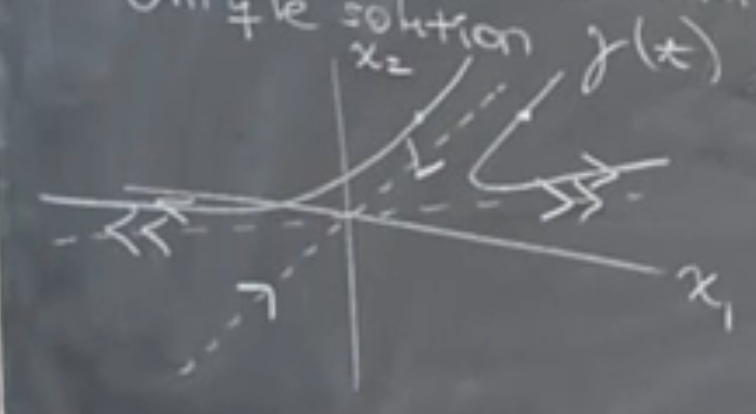
\includegraphics[width=0.8\textwidth]{Images/Lecture 1 Trajectories.png}
    \end{figure}

    More strongly, we observe that the dynamics of $\frac{dx}{dt} = Ax$ are defined by the eigenvectors and eigenvalues of $A$.

    For a diagonalizable matrix in general, we will have (up to conjugation), $n$ different axes which are positively or negatively oriented and then trajectories will fall along linear combinations of these. 

    A more interesting question is \textbf{what conditions can fail for a matrix to be diagonalizable?}
    
    In the case where $A$ is diagonalizable, we know what to do: Change the basis so that $A = PDP^{-1}$. Focus on $y' = Dy$ 

    There are two other cases to consider:
    \begin{itemize}
        \item The eigenvalues of $A$ are not real (e.g. $A = \begin{pmatrix}
            0 & -1\\ 
            1 & 0
        \end{pmatrix}$). This is annoying but still solvable. 

        \item The eigenvalues of $A$ are \emph{deficient} (the geometric multiplicity is less than the algebraic multiplicity). (e.g. $A = \begin{pmatrix}
            1 & 1\\
            0 & 1
        \end{pmatrix}$)
    \end{itemize}

    \textbf{Example 3:} 
    \begin{align*}
        \frac{dx_1}{dt} &= x_1 + x_2\\
        \frac{dx_2}{dt} &= x_2
    \end{align*}

    First notice, that $\begin{pmatrix}
        1 & 1\\ 
        0 & 1
    \end{pmatrix}$ has an eigenvector corresponding to the solution 
    \[s_1(t) = e^t \begin{pmatrix}
        1\\0
    \end{pmatrix}\]
    But $\text{dim } N(A - I) = 1, \quad p(\lambda) = (1 - \lambda)^2$ 

    There is a trick: \emph{Jordan Canonical Form.} 

    We will let $s_1(t) = e^t u$ and introduce a new solution:
    \[s_2(t) = te^t u + e^t v\]
    where $v$ is unspecified (but we will find a condition to make this a real solution.)

    Of course, 
    \[s_2(t) = ts_1(t) = e^t v\]
    By the product rule, 
    \[s_2'(t) = s_1(t) + ts_1'(t) + e^tv\]
    For this to be a solution, we want 
    \[\frac{d}{dt}s_2(t) - As_2(t) = 0\]
    Thus
    \[s_2'(t) = As_2(t) = A(ts_1(t) + e^t v) = tAs_1(t) + e^t Av\]
    Putting these together, 
    \[s_1(t) + ts_1'(t) + e^t v = tAs_1(t) + e^t v\]
    But notice that $ts_1'(t) = tAs_1(t)$ so we have 
    \[s_1(t) + e^tv - e^tAv = e^t u + e^t v - e^t Av = 0\]
    Factoring out an $e^t$, we have 
    \[u + v - Av = 0 \implies (A - I)v =u\]
    which is just a generalized eigenvalue. 

    Thus, if we can find a $v$ such that $(A - I)v = u$, then we have a solution.

    How do we know such a $v$ exists? Because it is Jordan Canonical Form. 

    \textbf{Exercise:} Find the solutions corresponding to 
    \[A = \begin{pmatrix}
        1 & 1 & 0\\ 
        0 & 1 & 1\\
        0 & 0 & 1
    \end{pmatrix}\]

\section{Jan 26:}
\subsection*{Jordan Canonical Form}
    Let $V$ be a finite dimensional vector space over $\C$. (Algebraic reasons: we want the characteristic polynomial to split). Let $A$ be a linear transformation of $V$ to itself. 

    Ideally, find a basis for $V$ such that 
    \[(A)_{\mathcal{B}} = \begin{pmatrix}
        \lambda_1\\ 
        & \lambda_2\\ 
        & & \ddots\\ 
        & & & \lambda_d
    \end{pmatrix}\] 
    (i.e. $A$ is diagonalizable)
    where $\lambda_i$'s are the eigenvalues of $A$ and 
    \[p(\lambda) = \det(A -\lambda I) \qquad (\text{ or } \det(\lambda I - A))\]
    is the n-th degree polynomial with coefficients in $\C$.

    By the FTOA, 
    \[p(\lambda) = (-1)^n (\lambda - \lambda_1)\dots(\lambda - \lambda_n)\]
    where the lambdas could be repeated. But this is also equal to 
    \[(-1)^n (\lambda - \lambda_1)^{d_1} (\lambda - \lambda_2)^{d_2} \dots (\lambda 
    - \lambda_k)^{d_k}\]
    where the lambdas are distinct and $d_i$ is the algebraic multiplicity of $\lambda_i$. 

    We denote $E_i = N(A - \lambda_i I), \; g_i = \dim E_i = \text{ geometric multiplicity of } \lambda_i$.

    \textbf{Theorem:} $g_i \leq d_i$

    \textbf{Theorem:} The map $A$ is diagonalizable iff $g_i = d_i$ for each $\lambda_i$. (the geometric multiplicity is equal to the algebraic multiplicity)

    \textbf{Example:} if there are $n$-distinct eigenvalues 
    \[p(\lambda) = (-1)^n (\lambda - \lambda_1)^1 (\lambda - \lambda_2)^1 \dots (\lambda - \lambda_k)^1\] 
    then $g_i = d_i = 1$, so diagonalizes. 
    
    \textbf{Example:} $A = \begin{pmatrix}
        1 & 1\\ 
        0 & 1
    \end{pmatrix}, \; p(\lambda) = (1 -\lambda)^2, \; \lambda_1$ has algebraic multiplicity of 2 but $\dim N(A - I) = \dim N\begin{pmatrix}
        0 & 1\\
        0 & 0
    \end{pmatrix} = 1$. Since $1 < 2$, $A$ is not diagonalizable. 

    \textbf{Jordan Canonical Form:} Let $V$ be a finite dimensional vector space over $\C$, let $A$ be a linear map from $V$ to itself. Then $B$ decomposes a direct sum of $A$-invariant subspaces $V = \bigoplus_{i=1}^k W_i$ such that for each $i$, there exists a basis $\mathcal{B}_i$ for which 
    \[(A \mid w_i)_{\mathcal{B}} = \begin{pmatrix}
        \lambda & 1\\ 
        & \lambda & 1\\ 
        & & \lambda & 1\\ 
        & & & \ddots\\ 
        & & & & \lambda
    \end{pmatrix}\]  
    where $\lambda$ is an eigenvalue of $A$. 

    \emph{Observation:} For any map $A$ from $V$ to itself, there exists a basis $\mathcal{B}$ of $V$ for which 
    \[(A)_{\mathcal{B}} = \begin{pmatrix}
        J_1\\ 
        & J_2\\ 
        & & \ddots\\ 
        & & & J_k
    \end{pmatrix}\] 
    where each $J_i = \begin{pmatrix}
        \lambda & 1\\ 
        & \lambda & 1\\ 
        & & \lambda & 1\\ 
        & & & \ddots\\ 
        & & & & \lambda
    \end{pmatrix}$ is called a \emph{Jordan Block.} 

    For any linear map $A$, $A$ preserves a complete \emph{flag} 
    \[0 \lneq z_1 \lneq z_1 \lneq \dots \lneq z_n = V\] 
    with $\dim(Z_{i+1}, Z_i) = 1$, every linear map up to conjugation is upper triangular. 

    \emph{Example:} 
    \[\begin{pmatrix}
        0\\0\\0
    \end{pmatrix} \lneq \begin{pmatrix}
        z_1\\ 0\\0
    \end{pmatrix} \lneq \begin{pmatrix}
        z_1\\ z_2\\0
    \end{pmatrix}\lneq  \begin{pmatrix}
        z_1\\ z_2\\z_3
    \end{pmatrix} = \C^3\] 

    \textbf{Jodan Chevalley Decomposition:}
    More strongly, this tells us that \emph{each linear map decomposes as a sum of a diagonalizable part and a nilpotent part.} i.e. $A = D + N$ where $D$ is diagonalizable and $N$ is nilpotent. Further, the pieces commute. 

    \emph{Example:} 
    \[A = \begin{pmatrix}
        2 & 1 & 0\\ 
        0 & 2 & 1\\ 
        0 & 0 & 2
    \end{pmatrix} = \underbrace{\begin{pmatrix}
        2 & 0 & 0\\ 
        0 & 2& 0\\ 
        0 & 0 & 2
    \end{pmatrix}}_{D} + \underbrace{\begin{pmatrix}
        0 & 1 & 0\\ 
        0 & 0 & 1\\ 
        0 & 0 & 0
    \end{pmatrix}}_{N}\] 
    and $DN = ND$. 

    Put differently, all of these pieces are cyclic in the sense that they are generated by a single vector and its iterates under the map $A$. 

    \textbf{Claim:} $\C^3 = \C\{e_3, Ae_3, A^2 e_3\}$ 

    \emph{Proof:} 
    \[e_3 = \begin{pmatrix}
        0\\0\\1
    \end{pmatrix}, \quad Ae_3 = 2e_3 + e_2, \quad A^2 e_3 = \dots\]

    \emph{Example:} 
    \[A = \begin{pmatrix}
        3 & 2 & -3\\ 
        1 & 3 & -2\\ 
        1 & 1 & 0
    \end{pmatrix}\]
    has char. poly. $p(\lambda) = (2 - \lambda)^3$ which only has eigenvalue $\lambda = 2$. Thus, this is not diagonalizable ($\dim N(A - 2I) \neq 3$) 

    But what we can do is look at powers of $A - 2I$:
    \begin{align*}
        A - 2I &= \begin{pmatrix}
            1 & 2 & -3\\ 
            1 & 1 & -2\\ 
            1 & 1 & -2
        \end{pmatrix}\\ 
        (A - 2I)^2 &= \begin{pmatrix}
            0 & 1 & -1\\ 
            0 & 1 & -1\\ 
            0 & 1 & -1
        \end{pmatrix}\\ 
        (A - 2I)^3 &= 0
    \end{align*} 
    This makes sense because of nilpotency and the Cayley Hamilton Theorem. 

    \textbf{Cayley Hamilton Theorem:} If there is a linear map $A$, then $p(A) = 0$ where $p(\lambda)$ is characteristic polynomial.

    Thus, we just choose a vector that is not in the nullspace of $N((A- 2I)^2)$ (the previous non-zero term), say $u = \begin{pmatrix}
        1\\1\\1
    \end{pmatrix}$. 

    Then, $\{(A - 2I)^2u, (A-2I)u, u\}$ will be a Jordan basis. 

    \emph{Proof:} denote $v_1 = (A-2I)^2 u, v_2 = (A-2I)u, v_3 = u$. Then 
    \begin{align*}
        (A- 2I)v_1 &= (A-2I)^3 v_1 = 0 \implies Av_1 - 2v_1 = 0 \implies v_1 \text{ eigenvector of } A\\ 
        Av_2 &= (A - 2I)v_2 + 2Iv_2 = v_1 + 2v_2\\ 
        Av_3 &= (A - 2I)v_3 + 2Iv_3 = v_2 + 2v_3
    \end{align*}
    so in regard to this basis, 
    \[(A)_{\mathcal{B}} = \begin{pmatrix}
        2 & 1 & 0\\ 
        0 & 2 & 0\\
        0 & 0 & 2
    \end{pmatrix}\]

\section{Jan 29:}
\subsection*{Recall} 
    Jordan Canonical Form says that, up to similarity, every matrix in $\C^{n \times m}$ looks like 
    \[\begin{pmatrix}
        J_1\\ 
        & J_2\\
        & & \ddots\\
        & & & J_k
    \end{pmatrix}\] 
    where each $J_i$ is a \emph{Jordan Block} of the form 
    \[J_i = \begin{pmatrix}
        \lambda_i & 1\\ 
        & \lambda_i & 1\\
        & & \ddots\\
        & & & \lambda_i
    \end{pmatrix}\]
    which means that any operator can be written as a diagonal and nilpotent part:
    \[A = D + N\]
    where $D$ and $N$ commute.  

    This discussion was originally motivated by the problem 
    \[\frac{d}{dx} = Ax\]
    with constraint $x(0) = x_0$, $x(t)$ a function into $\R^n$, and $A$ some real $n \times n$ matrix

    \textbf{Theorem:} For any choice of $x_0 \in \R^n$ and $A \in \R^{n \times n}$, there exists a unique solution $x(t)$ to the above problem.

    In some sense, this gives us a map. Fix $A \in \R^{n \times n}$, choose $x(0) = x_0$, $x_0 \in \R^n$, and $t \in \R$. Then 
    \[\theta(t, x_0) = x(t)\]
    where $x(t)$ is the solution to $\frac{d}{dt}x = Ax$ with $x(0) = x_0$.

    (i.e. There is some trajectory $x(t)$ which passes through the point $x_0 = x(0)$ representing a flow) 
    
    Further, this flow gives us an $\R$-action: 
    \[\theta(t, x_0) = x(t)\] 

    \textbf{Recall:} Let $G$ be a group. Let $X$ be a set. We say a function $\alpha: G \times X \to X$ is a \emph{group action} if 
    \begin{enumerate}
        \item $\alpha(1, x) = x$, for all $x \in X$ 
        \item $\alpha(g, \alpha(h, x)) = \alpha(gh, x)$ for all $g, h \in G$ and $x \in X$
    \end{enumerate}

    Also note that the definition of a group action is equivalent to saying there is a homomorphism from $G \to \text{Sym}(X)$ 

    In this case, our group is $\R$. So the flow gives us a homomorphism from $\R \to \text{Diff}(\R^n)$ 
    (the \emph{diffeomorphism groups}, a collection of infinitely differentiable functions)

    We can imagine the trajectory-flow situation as the map $(t, x_0) \mapsto \theta(t, x_0)$ where $t$ refers to the movement along the trajectory. Thus, $\theta(0, x_0)$ refers to \emph{not} moving along the trajectory so $\theta(0, x_0) = x_0$ -- exactly in line with our first group action condition. 

    Now consider $\theta(t + s, x_0)$. 

    \begin{tikzpicture}
        % Draw the curved line
        \draw (0,0) to [bend left=20] (10,0);
    
        % Mark the dots at 30%, 60%, and 90% of the line
        \fill (3,0) circle (2pt) node[below] {$x_0$};
        \fill (6,0) circle (2pt);
        \fill (9,0) circle (2pt);
    
        % Draw the red arrow from the first dot to the second dot
        \draw[->, red] (3,0) -- (6,0) node[midway,above] {$s$};
    
        % Draw the blue arrow from the second dot to the third dot
        \draw[->, blue] (6,0) -- (9,0) node[midway,above] {$t$};
    \end{tikzpicture}

    We notice that moving $t + s$ corresponds to moving $s$ then moving $t$ But, the final point is the same as if we had simply moved a distance of $t$ from the second point: 
    \[\theta(t + s, x_0) = \theta(s, \theta(t, x_0))\]
 
    \emph{Proof:} Show that it is the unique solution corresponding to the initial value problem $\frac{d}{dt}x = Ax$ with $x(0) = x_0$. Define $y(t) = x(t + s)$ for some fixed $s$. Claim $\frac{dy}{dt} = Ay$ and $y(0) = x(s)$. (This is called the \emph{translation lemma})

    Notice too, this is exactly the second group action condition. Thus, we have an $\R$-action. More generally, for any $A \in \R^{n\times n}$, we get an induced $\R$-action on $\R^n$, given by flowing along trajectories:
    \[\R \to \text{Diff}(\R^n)\]
    but in fact, we can do better and heavily restrict the target group by looking at the solutions to $\frac{d}{dt}x = Ax$. 

    Let's fix a time $t \in \R$, then 
    \[\theta_t: \R^n \rightarrowtail \R^n\]
    (i.e. there is a bijection from $\R^n$ to $\R^n$)

    And 
    \[\theta_t(x_0 + y_0) = \theta_t(x_0) + \theta_t(y_0)\] 
    So each $\theta_t$ is an (invertible) linear map. 

    Thus, we can restrict the homomorphism to 
    \[\theta: \R \to \GL(\R^n)\] 
    (the general linear group on $\R^n$) 

    \textbf{Definition:} $F: \R^n \rightarrowtail \R^n$ is a \emph{diffeomorphism} iff it has infinitely differential partial derivatives and is invertible with same property. 

    More precisely, the Jacobian is non-zero. Heuristically, it is a smooth, bijective, invertible map. 

    \textbf{Definition:} Let $V$ be a finite dimensional vector space, $\R^n$, $T \in \GL(\R^n)$ iff $T$ is linear and has a linear inverse iff $\det(T) \neq 0$.  

    \textbf{Definition:} A one parameter subgroup is a homomorphism from $\R \overset{\alpha}{\longrightarrow} \GL(n, \R)$ 
    
    \emph{Example:} Every matrix $A$ gives us a a one parameter subgroup.

    \emph{Example:} With
    \[\frac{d}{dt}\begin{pmatrix}
        x_1\\x_2
    \end{pmatrix} = \begin{pmatrix}
        2 & 0\\ 
        0 & 1/2
    \end{pmatrix} \begin{pmatrix}
        x_1\\ x_2
    \end{pmatrix}\]
    and $x(0) = x_0 = \begin{pmatrix}
        a\\b
    \end{pmatrix}$, solve the system. 
    
    The general solution is just 
    \[x(t) = ae^{2t} \begin{pmatrix}
        1\\0
    \end{pmatrix} + be^{\frac{1}{2}t} \begin{pmatrix}
        0\\1
    \end{pmatrix} = \begin{pmatrix}
        e^{2t} & 0\\ 
        0 & e^{\frac{1}{2}t}
    \end{pmatrix} \begin{pmatrix}
        a\\b
    \end{pmatrix}\]

    Note that $\theta(t) = \begin{pmatrix}
        e^{2t} & 0\\ 
        0 & e^{\frac{1}{2}t}
    \end{pmatrix}$ is a group homomorphism $\R \to \GL(2, \R)$! 
    \[\theta(t + s) = \theta(t) \theta(s)\]

    Then if 
    \begin{align*}
        x(t) &= M(t) x_0, \; M(0) = I\\ 
        \frac{dx}{dt} &= M'(t)x_0 = AM(t)x_0\\ 
        &\implies M'(t) = AM(t)
    \end{align*}
    which tells us that for a one parameter subgroup, $\theta(s + t) = \theta(s) \theta(t)$, $\theta$ takes addition into multiplication. 

    \textbf{Matrix Exponential:} 

    Let $A \in \C^{n\times n}$. Define 
    \[e^A = I_n + A + \frac{1}{2} A^2 + \frac{1}{3!} A^3 + \dots = \sum_{n=0}^{\infty} \frac{1}{n!}A^n\]

    \emph{Justification of well-defined:}
    \[\norm{e^A} \leq \sum_{n=0}^{\infty} \frac{1}{n!} \norm{A}^n < \infty\] 

    So $e^A$ always makes sense and we have 
    \begin{align*}
        \R &\to GL(n, r)\\
        t &\mapsto e^{tA}
    \end{align*} 
    gives a one parameter subgroup.

\section{Jan 31:}
    \textbf{Recall:} The matrix exponential arises from an $n \times n$ (say real) matrix which gives a homomorphism $\phi: \R \to \GL(n, \R)$. $\phi(\cdot)$ is the flow of the ODE $\frac{dx}{dt} = Ax$ when 
    \[x(t) = \phi(t) x_0, \; x_0 \in \R^n\]
    with
    \begin{align*}
        \phi(t + s) &= \phi(t) \phi(s)\\ 
        \frac{d\phi}{dt}(t) = A\phi(t)\\ 
        \phi(0) = I
    \end{align*}
    
    Further, the existence of $\phi$ is guaranteed by existence and uniqueness of ODEs. 

    What exactly is $\phi$? Precisely the matrix exponential:
    \[\phi(t) = e^{tA} = \sum_{n=0}^{\infty} \frac{1}{n!}(tA)^n\]

    \begin{tbox}{\textbf{Claim:} $x(t) = e^{tA}x_0$ solves $\frac{dx}{dt} = Ax$, $x(0) = x_0$}
        \emph{Proof:} 
        
        First we verify the initial condition: 
        \[x(0) = e^{0A}x_0 = (I + 0 + 0 + \dots) x_0 = x_0\]
        (this is a little bit of an abuse of notation saying $I = 1$)

        Now taking the derivative:
        \begin{align*}
            \frac{dx}{dt} &= \frac{d}{dx}(1 + tA + \frac{1}{2}t^2 A^2 + \frac{1}{3!}t^3 A^3 + \dots)x_0\\ 
            &= (0 + A + tA^2 + \frac{1}{2}t^2 A^3 + \dots)x_0\\
            &= A(1 + tA + \frac{1}{2!}t^2 A^2 + \dots)x_0
            &= Ae^{tA}x_0\\ 
            &= Ax(t)
        \end{align*}

        So it is a solution to the ODE.
    \end{tbox}

    Consequently, we know 
    \[e^{tA}e^{sA} = e^{(t+s)A}\] 
    because of the homomorphism conditions. But we can also say $\phi(0) = I$ and $\phi'(0) = A$. 

    \textbf{Example:} 
    \[\frac{dx}{dt} = \begin{pmatrix}
        2 & 0\\ 
        0 & 1/2
    \end{pmatrix}x \implies e^{tA} = \begin{pmatrix}
        e^{2t} & 0\\ 
        0 & e^{t/2}
    \end{pmatrix}\]

    \textbf{Example:} 
    \[\frac{dx}{dt} = Ax = \begin{pmatrix}
        3 & -4\\ 
        2 & -3
    \end{pmatrix} x\]

    \emph{Note:}
    \begin{align*}
        e^{PBP^{-1}} &= 1 + PBP^{-1} + \frac{1}{2!}(PBP^{-1})^2 + \frac{1}{3!}(PBP^{-1}) + \dots\\ 
        &= 1 + PBP^{-1} + \frac{1}{2}PB^2 P^{-1} + \frac{1}{3!} PB^3P^{-1} + \dots\\ 
        &= Pe^BP^{-1}
    \end{align*}

    This leads to the observation that calculating $e^{tA}$ with $A$ diagonalizable, we can just write 
    \[e^{tA} = e^{tPDP^{-1}} = Pe^{tD}P^{-1}\]

    Thus for $A = \begin{pmatrix}
        3 & -4\\ 
        2 & -3
    \end{pmatrix}$, we have $\lambda_1 = -1, \; v_1 = \begin{pmatrix}
        1\\1
    \end{pmatrix}, \lambda_2 = 1, \; v_2 = \begin{pmatrix}
        2\\1
    \end{pmatrix}$

    Currently, we have $(A)_{\mathcal{B}} = A$ where $\mathcal{B} = \{e_1, e_2\}$. We introduce a new basis $\gamma = \{v_1, v_2\}$ and write $A = DPP^{-1}$ by 
    \[(A)_{\mathcal{B}} = (I)^{\gamma}_{\mathcal{B}} (A)_{\gamma} [(I)^{\gamma}_{\mathcal{B}}]^{-1}\] 
    so 
    \[\begin{pmatrix}
        3 & -4\\ 
        2 & -3
    \end{pmatrix} = \begin{pmatrix}
        1 & 2\\ 
        1 & 1
    \end{pmatrix} \begin{pmatrix}
        -1 & 0\\ 
        0 & 1
    \end{pmatrix} \begin{pmatrix}
        1 & 2\\ 
        1 & 1
    \end{pmatrix}^{-1}\] 
    Thus, 
    \[e^{tA} = Pe^{tD} P^{-1} = \begin{pmatrix}
        1 & 2\\ 
        1 & 1
    \end{pmatrix} \begin{pmatrix}
        e^{-t} & 0\\
        0 & e^t
    \end{pmatrix} \begin{pmatrix}
        1 & 2\\ 
        1 & 1
    \end{pmatrix} = \begin{pmatrix}
        e^{-t} + 2e^t & 2e^{-t} + 2e^t\\ 
        e^{-t} + e^t & 2e^{-t} + e^t
    \end{pmatrix}\]
    Then if we want to solve the initial value problem (say $x(0) = \begin{pmatrix}
        4\\3
    \end{pmatrix}$) then we just have 
    \[x(t) = e^{tA}x_0 =\begin{pmatrix}
        e^{-t} + 2e^t & 2e^{-t} + 2e^t\\ 
        e^{-t} + e^t & 2e^{-t} + e^t
    \end{pmatrix}\begin{pmatrix}
        4\\3
    \end{pmatrix} = \begin{pmatrix}
        10e^{-t} + 14e^t\\ 
        10e^{-t} + 7e^t
    \end{pmatrix}\]

    We would like to generalize more exponential properties (such as saying $e^{A+B} = e^A e^B = e^B e^A$). But in general, this almost \emph{never} holds. Except under a very special condition!

    \begin{tbox}{\textbf{Theorem:} Let $A, B$ be matrices that commute, i.e. $AB = BA$. Then $e^A e^B = e^B e^A = e^{A + B}$}
        \emph{Calculation:}

        \begin{align*}
            e^A e^B &= (I + A + \frac{1}{2}A^2 + \dots)(I + B + \frac{1}{2}B^2 + \dots)\\ 
            &= I + (A + B) + (\frac{1}{2!}A^2 + AB + \frac{1}{2!} B^2) + (\frac{1}{3!}A^3 + \frac{1}{2!\, 1!}A^2B + \frac{1}{2!\, 1!}AB^2 + \frac{1}{3!}B^3) + \dots\\
            &= \sum_{n=0}^{\infty} \left(\sum_{k=0}^n \frac{1}{k!(n - k)!}A^{n-k} B^k\right)\\ 
            &= \sum_{n=0}^{\infty} \left(\frac{1}{n!} \sum_{k=0}^n \frac{n!}{k!(n - k)!}A^{n-k} B^k\right)\\ 
            &= \sum_{n=0}^{\infty} \left(\frac{1}{n!} \sum_{k=0}^n \binom{n}{k}A^{n-k} B^k\right)\\
            &= \sum_{n=0}^{\infty} \frac{1}{n!}(A + B)^n \qquad (\text{note that this needs commutativity!!})
        \end{align*}
    \end{tbox}

    \textbf{Example:} $\frac{dx}{dt} = \begin{pmatrix}
        1 & a\\ 
        0 & 1
    \end{pmatrix}x$
    \begin{align*}
        e^{tA} &= e^{t(I + N)} \qquad \text{(Jordan Canonical!)}\\ 
            &= e^{tI}e^{tN}\\ 
            &= \begin{pmatrix}
                e^t & 0\\ 
                0 & e^t
            \end{pmatrix} \begin{pmatrix}
                1 & ta\\ 
                0 & 1
            \end{pmatrix}
    \end{align*}

    Notice that the Nilpotent part will always be a finite sum. In the example above $N = I + tN$ in the Taylor Expansion (because $N^2 = 0$).

    And indeed, we can generalize this. Up to conjugation, 
    \[e^{tA} \sim e^{tD} e^{tN}\]
    for some diagonal and nilpotent matrices $D$ and $N$.

\section{Feb 2:}
    \textbf{Recall:} 
    
    \emph{Example:} With $A = \begin{pmatrix}
        \lambda & 0\\ 
        0 & -\lambda
    \end{pmatrix}$, $\lambda \in \R$, then 
    \[e^{tA} = \begin{pmatrix}
        e^{\lambda t} & 0\\ 
        0 & e^{-\lambda t}
    \end{pmatrix}\]
    Its determinant is $1$ so $e^{tA} \in \SL(2, \R)$. This has some cool properties: because it is traceless, it preserves volume and up to conjugation, these matrices preserve the Lorentzian product (Physics) 
    \[\brak{\begin{pmatrix}
        x_1\\x_2
    \end{pmatrix}, \begin{pmatrix}
        y_1\\y_2
    \end{pmatrix}} = x_1 y_1 - x_2 y_2\] 
    so are of the form $\begin{pmatrix}
        \cosh t & \sinh t\\
        \sinh t & \cosh t
    \end{pmatrix}$

    \emph{Example:} $A = \begin{pmatrix}
        0 & -1\\ 
        1 & 0
    \end{pmatrix}, \lambda = \pm i$ so we cannot diagonalize over the reals. 

    \[e^{tA} = \sum_{n=0}^{\infty} \frac{1}{n!}(tA)^n\] 
    but 
    \[A^2 = \begin{pmatrix}
        -1 & 0\\ 
        0 & -1
    \end{pmatrix} = -I \implies A^3 = A, \; A^4 = I\]
    so 
    \begin{align*}
        e^{tA} &= \frac{1}{0!} I + \frac{1}{1!}tA - \frac{1}{2!}t^2 I - \frac{1}{3!}t^3A + \frac{1}{4!}t^4 I \pm \dots\\ 
            &= \sum_{n=0}^{\infty} \frac{(-1)^n}{(2n!)} t^{2n} I + \sum_{n=0}^{\infty} \frac{(-1)^n}{(2n + 1)!} t^{2n + 1} A\\ 
            &= \cos(t)I + \sin(t)A\\ 
            &= \begin{pmatrix}
                \cos t & -\sin t\\
                \sin t & \cos t
            \end{pmatrix} \in SO(2, \R)
    \end{align*}

    (Remark: You have absolute convergence on compact subspaces so the summation splitting is well-defined)

    \textbf{Definition:} $SO(2, \R)$ is the group of $2\times 2$ matrices that preserve the standard euclidean product $\brak{\begin{pmatrix}
        x_1\\x_2
    \end{pmatrix}, \begin{pmatrix}
        y_1\\y_2
    \end{pmatrix}} = x_1 y_1 + x_2 y_2$

    Further, $\det(e^{tA}) = \cos^2 t+ \sin^2 t = 1$ 

    This leads to a generalization: Given a matrix, you get a whole family of matrices in a group, on which you can impose conditions on the input matrix to land in certain groups. 

    A matrix group $H$ then looks at one parameter families about $1 \in G$. 
    \[\gamma: \R \to G\]
    where $\gamma'(0)$ is in the Tangent space of $G$ so $\exp$ maps the tangent space at $1 \in G$ to the open ball about $1 \in G$. 

    \emph{Example:}
     \[\begin{pmatrix}
        0 & a\\ 
        0 & 0
     \end{pmatrix} \oplus \begin{pmatrix}
        0 & -b\\ 
        b & 0
     \end{pmatrix} \oplus \begin{pmatrix}
        c & 0\\ 
        0 & -c
     \end{pmatrix} \overset{\exp}{\longrightarrow} \SL(2, \R)\]
    \textbf{Example:} $A = \begin{pmatrix}
        -1/2 & 1\\ 
        1 & -1/2
    \end{pmatrix}$ so you can just decompose it into 
    \[A = \begin{pmatrix}
        -1/2 & 0\\ 
        0 & -1/2
    \end{pmatrix} + \begin{pmatrix}
        0 & -1\\ 
        1 & 0
    \end{pmatrix}\]
    Since the two blocks ($R, S$) commute, 
    \[e^{tA} = e^{tR} e^{tS} = e^{-t/2}\begin{pmatrix}
        \cos t & -\sin t\\ 
        \sin t & \cos t
    \end{pmatrix}\]

    \textbf{Claim:} We end up having $e^{tA}$ is invertible and lands in $\GL(n, \R)$ or $\GL(n, \C)$ (note: only one of those is surjective)

    \begin{tbox}{\textbf{Theorem:} $\det(e^A) = e^{\tr A}$ for any matrix $A \in M_n(\C)$}
        \emph{Proof:} (Sketch - diagonalize and invoke density of diagonalizable matrices in $\GL(n, \R)$)

        Using Jordan Canonical Form: note that $\det$ is conjugation invariant so 
        \begin{align*}
            \det(e^A) &= \det(Pe^{A}P^{-1})\\ 
                &= \det(e^{PAP^{-1}})\\ 
                &= \det(e^{D + N})\\ 
                &= \det(e^D)\det(e^N)\\ 
                &= e^{\lambda_1 + \lambda_2 + \dots + \lambda_n} \cdot 1\\
                &= e^{\tr A}
        \end{align*}
        (because $D = \begin{pmatrix}
            e^{\lambda_1}\\ 
            & e^{\lambda_2}\\
            & & \ddots\\
            & & & e^{\lambda_n}
        \end{pmatrix}$ and $e^N = 1 + N + \frac{1}{2}N^2 + \dots$ is an upper triangular matrix with $1$'s on the diagonal. Also, $\tr A = \sum_{i=1}^n \lambda_i$ and $\det A = \prod_{i=1}^n \lambda_i$)
    \end{tbox}

    \emph{Remark:} this is one of the first hints at a fundamental relation between Lie groups and Lie algebras 

    An immediate consequence is that $\exp: M_n(\R) \to \GL(n, \R)$ lies in the identity component of $\GL(n, \R)$ (i.e. $\det(e^A) > 0$)

   

\section{Feb 05:}
    \begin{tbox}{\textbf{Theorem:} Let $A(t)$ be a smooth family of matrices in $\GL(2, \R)$ and $A(0) = I$. Then 
        \[\frac{d}{dt}\bigg\vert_{t =0 } \det A(t) = \tr A'(0)\]}
        \emph{Proof:} 

        Let $A(t)$ be smooth with $A(0) = I$ and $A'(0) = B$. Consider the curve $\gamma(t) = e^{tB}$.

        Notice that up to first order, $A(t)$ and $\gamma(t)$ agree:
        \begin{align*}
            A(0) &= \gamma(0) = I\\ 
            A'(0) &= B = \gamma'(0)
        \end{align*} 
        put differently,
        \begin{align*}
            A(t) &= I + tB + O(t^2)\\ 
            \gamma(t) &= I + tB + O(t^2)
        \end{align*}
        Taking the derivative linearizes the curves, so we can safely ignore higher order terms. 

        Then taking the derivatives, 
        \[\frac{d}{dt}\bigg\vert_{t=0} \det A(t) = \frac{d}{dt}\bigg\vert_{t=0} \det \gamma(t)\]
        (Note that this is actually a chain rule property assuming $\det: M_n(\R) \to \R$ is differentiable at $I$). 

        Because $\det$ is differentiable at $A(0) = \gamma(0)$ ($\det$ is polynomial in entries of input matrix), we can use the chain rule. 
        \[\frac{d}{dt}\bigg\vert_{t=0} A(t) = D(\det)_{I} \circ \frac{d}{dt}\bigg\vert_{t=0} A(t) = D(\det)_I \frac{d}{dt}\bigg\vert_{t=0} \gamma(t) = \frac{d}{dt}\bigg\vert_{t=0} \det \gamma(t)\]

        Since this is a 1-parameter subgroup, 
        \[\frac{d}{dt}\bigg\vert_{t=0} \det \gamma(t) = \frac{d}{dt}\bigg\vert_{t=0} \det e^{tB} = \frac{d}{dt}\bigg\vert_{t=0} e^{\tr(tB)}\]
        by the earlier theorem. Then, 
        \[\frac{d}{dt}\bigg\vert_{t=0} e^{\tr(tB)} = (e^{\tr(tB)} \bigg\vert_{t=0}) \cdot \frac{d}{dt}\bigg\vert_{t=0} \tr(tB) = \tr B \]
        (Notice that $\tr(tB) = \sum_{i=1}^n tB_{ii}$ so $\frac{d}{dt}\bigg\vert_{t=0} \tr(tB) = \sum_{i=1}^n B_{ii} = \tr B$)
    \end{tbox}

    We can represent these relationships by a set of commutative diagrams:
    
    \[\begin{tikzcd}
            G \arrow{r}{\phi} & H\\ 
            g \arrow[hookrightarrow]{u}{\exp} \arrow{r}{d\phi} 
            & h \arrow[hookrightarrow]{u}{\exp}
        \end{tikzcd} \qquad 
        \begin{tikzcd}
            \GL(n, \R) \arrow{r}{\det} & \R^*\\
            M_n(\R) \arrow[hookrightarrow]{u}{\exp} \arrow{r}{\tr}  
            & \R \arrow[hookrightarrow]{u}{\exp}
        \end{tikzcd}
    \]

    This hints at deep concept of lie homomorphisms on a group level and algebra level

    \textbf{Definition:} Let $G \subseteq \GL(n, \C)$ be a group of matrices. We say $G$ is a \emph{matrix group} if it is a smooth submanifold of $\GL(n, \C)$ (i.e. at every point $\mathfrak{g} \in G$, we can find a ``patch'' $U \subseteq \R^k \biject \phi(I) \subseteq G$)

    \begin{figure}
        \centering
        \includegraphics[width=0.5\textwidth]{Images/Feb 5 manifold.png}
    \end{figure}

    We want to do this in such a way that if we have two charts 
    \begin{align*}
        \phi: U \biject \phi(U) \subseteq G\\ 
        \psi: V \biject \psi(V) \subseteq G
    \end{align*}
    and $U \cap V$, 
    
    \[\begin{tikzcd}
        & (U \cap V) \arrow[hook, two heads]{dl}{\phi} \arrow[hook, two heads]{dr}{\psi} & \\ 
        \phi(U \cap V) \subseteq G \arrow[hook, two heads]{rr}{\psi \circ \phi^{-1}} 
            & & \psi(U \cap V) \subseteq G
    \end{tikzcd}\]

    where $(\psi \circ \phi^{-1})$ is smooth and differentiable infinitely many times. 

    \emph{Examples:}
    \begin{itemize}
        \item With 
        \[\SL(n, \C) \subseteq \GL(2, \R) = \left\{\begin{pmatrix}
            a & b\\ 
            c & d
        \end{pmatrix} \in \GL(2, \R) \bigg\vert \det -1\right\}\] 
        $\SL(n, \C)$ is a Lie group 

        \item 
        \[\SO(2, \R) \subseteq \GL(2, \R) = \{A \in \GL(2, \R) \big\vert \brak{Av, Aw} = \brak{v, w}\}\] $\forall v, x \in \R^2$ where $\brak{\cdot, \cdot}$ is euclidean inner product is a 1-dim Lie group 
    \end{itemize}

    These charts allow us to do calculus on our space $G$. 

    \emph{Example:} $G = \GL(n, \R)$ is an $n^2$-dimensional lie group. 
    
    \[\GL(n, \R) = \{A \in M_n(\R) \big\vert \det A \neq 0\}\]
    is a group with group law multiplication. We have closure because with $A, B \in \GL(n, \R)$, 
    \[\det(AB) = \det(A) \det(B) \neq 0\] 
    
    Why is this $n^2$-dimensional? Because $\det: \GL(n, \R) \to \R^*$ is a smooth map (continuous) so the neighborhood around a point is mapped to a neighborhood around $\det(A)$ in $\R^*$. 

    \emph{Example:} 
    \[\begin{pmatrix}
        1 & 0\\ 
        0 & 1
    \end{pmatrix} \in U = \left\{\begin{pmatrix}
        a & b\\ 
        c & d
    \end{pmatrix}: \abs{a - 1} < \varepsilon, \abs{d - 1} < \varepsilon, \abs{b - 1} < \varepsilon, \abs{c - 1} < \varepsilon\right\}\]

    \textbf{Example:} What is the definition of 
    \[G = \left\{\begin{pmatrix}
        \lambda_1\\ 
        & \lambda_2\\
        & & \lambda_3
    \end{pmatrix} \bigg\vert \lambda_1, \lambda_2, \lambda_3 > 0\right\} \subseteq \GL(3, \R)?\] 

    We can find a chart 
    \[\begin{pmatrix}
        \lambda_1\\ 
        & \lambda_2\\
        & & \lambda_3
    \end{pmatrix} \mapsto \begin{pmatrix}
        \lambda_1\\ 
        \lambda_2\\
        \lambda_3
    \end{pmatrix} \in \left\{\abs{\lambda_1 - 1} < \varepsilon, \abs{\lambda_2 - 1} < \varepsilon, \abs{\lambda_3 - 1} < \varepsilon\right\}\]

    \textbf{Example:} 
    \[\SL(3, \R) = \left\{\begin{pmatrix}
        a & b\\ 
        c & d
    \end{pmatrix} \bigg\vert ad - bc = 1\right\} \subseteq \GL(2, \R) = \left\{\begin{pmatrix}
        a & b\\ 
        c & d
    \end{pmatrix} \bigg\vert ad - bc \neq 0\right\}\]
    Coming up with an explicit chart is hard! But we can say the dimensionality is $3$. 

    Intuition: $a, b, d$ can be chosen freely but $c$ is determined by $\frac{ad - 1}{b} = c$ (note this breaks if $b = 0$!5)

\section{Feb 07:}
    \textbf{Recall:} Last time we looked at dimension of groups and the idea of a \emph{chart.} The point of a chart is to do calculus on $G$. 

    \textbf{Definition:} $G$ is a \emph{Lie group} if it is a smooth manifold and a group whose operation of multiplication and inversion are smooth maps.

    In our context, smoothness is automatically satisfied by ``nice'' subgroups of $\GL(n, \C)$

    Our ultimate goal is to construct a tangent space at $g = 1 \in G$: 
    \[g = \{B \in M_n(\C) \bigg\vert \quad B = \frac{d}{dt}\bigg\vert_{t = 0} \gamma(t), \; \gamma: \R\to G,\; \gamma(0) = 1\}\]
    ($\gamma$ is the \emph{lie algebra})

    Note that this definition does not include a notion of one parameter subgroups. However, you can in fact show that it is the same: \emph{Up to first order, every smooth path in $G$ is going to look exponential or like a one parameter subgroup.}

    \textbf{Example:} 
    \[G = \text{diag}^+(3, \R) = \begin{pmatrix}
        \lambda_1\\ 
        & \lambda_2\\
        & & \lambda_3
    \end{pmatrix} \text{ where } \lambda_i > 0\]

    Last time, we found that this is a 3-dimensional group. This notion should be reflected in the lie-algebra (the tangent space of the group) 

    We construct a family: 
    \begin{align*}
        \gamma(t) &= \begin{pmatrix}
            e^t\\ 
            & 1\\ 
            & & 1
        \end{pmatrix}, \quad \gamma(0) = 1\\ 
        \gamma'(0) &= \begin{pmatrix}
            1\\ 
            & 0\\ 
            & & 0
        \end{pmatrix} \in M_3(\R)\\ 
        \alpha(t) &= \begin{pmatrix}
            1\\ 
            & e^t\\ 
            & & 1
        \end{pmatrix} \implies \alpha'(0) = \begin{pmatrix}
            0\\ 
            & 1\\ 
            & & 0
        \end{pmatrix}\\ 
        \beta(t) &= \begin{pmatrix}
            1\\ 
            & 1\\ 
            & & e^t
        \end{pmatrix} \implies \beta'(0) = \begin{pmatrix}
            0\\ 
            & 0\\ 
            & & 1
        \end{pmatrix}
    \end{align*}
   
    So the general structure is:
    \[g = \left\{\begin{pmatrix}
        a\\ 
        & b\\
        & & c
    \end{pmatrix} \bigg\vert a, b, c \in \R\right\} = \begin{pmatrix}
        a\\ 
        & 0\\ 
        & & 0
    \end{pmatrix} \oplus \begin{pmatrix}
        0\\ 
        & b\\ 
        & & 0
    \end{pmatrix} \oplus \begin{pmatrix}
        0\\ 
        & 0\\ 
        & & c
    \end{pmatrix}\] 

    \textbf{Example:} $G = \SL(2, \R)$ is 3-dimensional so we expect $g$ to be 3-dimensional. 

    \[\SL(2, \R) = \{A \in \GL(2, \R) \big\vert \det A = 1\}\] 
    has $\gamma(t) \in \SL(2, \R), \; \gamma(0) = 1$. Differentiating, $\frac{d}{dt}\bigg\vert_{t=0} \tr \gamma'(0) = 0$ so 
    \[\sl(2, \R) = \{B \in M_2(\R)\big\vert \tr(B) = 0\}\]

    Thus for any matrix $B = \begin{pmatrix}
        a & b\\ 
        c & d
    \end{pmatrix}$, $\tr B = a + d = 0$, 
    \[\sl(2, \R) = \left\{\begin{pmatrix}
        a & b\\ 
        c & -a
    \end{pmatrix} \bigg\vert a, b, c \in \R\right\}\]  

    But this is not limited to $n=2$! In general, 
    \[\dim \sl(n, \R) = \dim \SL(n, \R) = n^2 - 1\]
    (because only the last diagonal entry is fixed)

    \begin{tbox}{ \emph{Claim:} $\dim \GL(n, \R) = n^2$}
        \emph{Proof:} $\GL(n, \R)$ is an open subset of $M_n(\R)$ which is $n^2$-dimensional.
    \end{tbox}

    \textbf{Natural question:} Why is the dimension of the lie group equal to the dimension of the lie algebra?
    
    \emph{Answer:} The exponential map is a local diffeomorphism. 
    \[F: \R^n\ to \R^n\]
    look at a fixed point $p$ and consider the Jacobian matrix at $p$, 
    \[dF \sim \begin{pmatrix}
        \frac{\partial F_1}{\partial x_1}\\ 
        \vdots\\
        \frac{\partial F_n}{\partial x_n} & \dots & \frac{\partial F_n}{\partial x_n}
    \end{pmatrix}\] 
    if $\det(\text{Jac})_p \neq 0$, then $F$ preserves dimension. 
    \[F \approx F(p) + \text{Jac}(p)(x - p) + \text{(higher order stuff)}\]

    So it suffices to calculate the derivative of $\exp: g \to G$ at $B = 0$ since we are interested in $\exp(0) = 1$.

    Calculate $d(\exp)_0(B) = \frac{d}{dt}\bigg\vert_{t=0} \exp(tB)$ where $\gamma(t) = tB$ is a particular path in $G$ with $\gamma(0) = 1$ and $\gamma'(0) = B$. 

    In fact, we know how to take this derivative. 
    \[\frac{d}{dt}\bigg\vert_{t=0} e^{tB} = B\]
    so technically, 
    \[d(\exp)_0: T_0\mathfrak{g}\to T_1G\] 
    but 
    \begin{tikzcd}
        T_0g \arrow{r} \arrow{d}{\simeq} & T_1G \arrow{d}{=}\\ 
        g \arrow[tail, two heads]{r}{I} & g
    \end{tikzcd}

    Say you have a point $\mathfrak{g} \in G$ and we want a chart about it. 
 
    A lie algebra has a local neighborhood around $0$. By exponentiation, we get to a local neighborhood around $1 \in G$, the lie group. If we want to get to $\mathfrak{g} \in G$, all it takes is a left multiplication because \emph{$G$ acts on itself by diffeomorphisms (smooth maps)}
    
    In general, you can always move from one point $g$ to another point $h$ by left multiplication,

    Most importantly, this tells us that any structure we want to induce on the Lie group can be induced on the Lie algebra (the tangent space at the identity)
     
    \textbf{Example:} Look at the KAN-decomposition chart of $\SL(2, \R)$: 
    \[\begin{pmatrix}
        \cos\theta & -\sin \theta\\ 
        \sin \theta & \cos \theta
    \end{pmatrix} \begin{pmatrix}
        \lambda & 0\\ 
        0 & \lambda^{-1}
    \end{pmatrix} \begin{pmatrix}
        1 & a\\ 
        0 & 1
    \end{pmatrix}\] 
    This happens to be the exponential map locally into $\SL(2, \R)$ (done carefully, this is actually a bijection!) 

    \textbf{Examples of Lie groups:}
    \begin{itemize}
        \item $G = \SO(3, \R)$ (the group of 3-dimensional rotations acting on $S^2$). What is the Lie algebra $\so(3, \R)$? We have two conditions: $\det A = 1$ and $\brak{Av, Aw} = \brak{v, w}$ where $\brak{\cdot, \cdot}$ is the euclidean inner product ($A^TA = 1$)
        
        Linearizing equation 1, we have $\tr(B) = 0$. To linearize equation 2, notice 
        \begin{align*}
            \frac{d}{dt}\bigg\vert_{t=0}([A(t)]^T A(t)) = 0 &\implies (\frac{d}{dt}\bigg\vert_{t=0} A(t)^T)A(0) + A(0)^T (\frac{d}{dt}\bigg\vert_{t=0}) = 0\\ 
            &\implies B^T + B= 0 
        \end{align*}

        Taking these two conditions together, we have a traceless, skew-symmetric matrix. (\textbf{Remark:} skew-symmetric implies traceless but the first condition is still necessary because reflections (for example) preserve inner product but not determinant). So we have a matrix of the form 
        \[\begin{pmatrix}
            0 & a & b\\ 
            -a & 0 & c\\ 
            -b & -c & 0
        \end{pmatrix}\]
        so $\dim(\so(3, \R)) = 3$
    \end{itemize}

    Finally, notice that we have not actually defined \emph{algebra.} Introduce the bracket: 
    \[[A, B] := \frac{d}{dt}\bigg\vert_{t=0} \frac{d}{ds}\bigg\vert_{s=0} e^{tA}e^{sB}e^{-tA}\] 
    and notice that $e^{tA}e^{sB}e^{-tA} \in G$ for all $s, t$ 

\section{Feb 09:} 
    Let's go back to the notion of the Lie Algebra. We have a vector space structure associated to the lie group. $g = T_1 G$, the tangent space at $1 \in G$. 

    This vector space also has an algebra structure: we can pair tangent vectors together. Let $A, B \in \mathfrak{g}$. Define
    \[[A, B] = \frac{d}{dt}\bigg\vert_{t=0} \frac{d}{ds}\bigg\vert_{s=0}e^{tA}e^{sB}e^{-tA}\]

    There are two (conflicting) interpretations:
    \begin{enumerate}
        \item failure to commute on the level of flows induced by $e^{tB}, e^{sA}$.
        \item infinitesimal derivative of the conjugation action 
    \end{enumerate}

    Looking at the calculation, we see that we are really doing conjugation by $e^{tB}$ applied to $e^{sA}$. 

    Taking derivatives, 
    \[[A, B] = \frac{d}{dt}\bigg\vert_{t=0} e^{tA} Be^{-tA}\] 
    but this is weird! $B \in \mathfrak{g}$ but $e^{tA}, e^{-tA} \in G$. This is the magic of the matrix group property. This is an ambient manifold allowing us to identify tangent vectors with elements of the group. 

    Regardless, 
    \[\frac{d}{dt}\bigg\vert_{t=0} e^{tA} Be^{-tA} = (ABe^{-tA} + e^{tA}(-BA)e^{-tA})\bigg\vert_{t=0} = AB - BA\]
    
    This gives us a way of taking tangent vectors to other tangent vectors ($g \times g \to g$). Further, this pairing is motivated by conjugation.

    \textbf{Note:} $[A, A] = AA - AA = 0$. (This is not surprising! Two flows generated by the same matrix will commute.)

    The bracket is also bilinear: 
    \begin{align*}
        [A + cB, D] &= (A + cB)D - D(A + cB)\\ 
        &= AD + cBD - DA - cDB\\ 
        & = AD - DA + c(BD - DB)\\ 
        &= [A, D] + c[B, D]
    \end{align*}

    Finally, 
    \[[X, [Y, Z]] + [Y, [Z, X]] + [Z, [X, Y]] =0\]
    for all $X, Y, Z \in \mathfrak{g}$. This is called the \emph{Jacobi identity}. 

    \textbf{Definition:} A vector space with a pairing $[\cdot, \cdot]:\mathfrak{g}\times\mathfrak{g}\to \mathfrak{g}$ denoted by $(\mathfrak{g}, [\cdot, \cdot])$ is called a \emph{Lie Algebra} iff it is:
    \begin{enumerate}
        \item Skew-symmetric ($[B, A] = -[A, B]$)
        \item Bilinear in both variables 
        \item Jacobi identity holds ($[X, [Y, Z]] + [Y, [Z, X]] + [Z, [X, Y]] = 0$)
    \end{enumerate}

    So we can think of this as 
    \[\begin{array}{c}
        G \to \Aut(G)\\ 
        g \mapsto ghg^{-1}
    \end{array}\]

    Now we have calculated the vector space structure, but not the algebraic structure. 

    \textbf{Examples:} 
    \begin{itemize}
        \item $(\R^n, +)$. Clearly, this is a group. We can look at $T_0\R^n = \R^n$ (this is the lie-algebra of $\R^n$ and the vector space). We want addition in $\R^n$ to commute so $[X, Y] = 0$. 
        
        Say we want to embed $\R^n \hookrightarrow \GL(\R^m)$? Just consider the exponential map:
        \[(\lambda_1, \lambda_2, \dots, \lambda_n) \mapsto \begin{pmatrix}
            e^{\lambda_1}\\ 
            & \lambda_2\\ 
            & & \ddots\\
            & & & e^{\lambda_n}
        \end{pmatrix}\]

        (This is exactly analogous to the mapping $\R \overset{\exp}{\to} \GL(1) \simeq \R^*$)

        If we specify to $\R^3$, 
        \[g =\left\{\begin{pmatrix}
                a\\ 
                & b\\ 
                & & c
            \end{pmatrix} \bigg\vert a, b, c \in \R \right\}\]
        and pair any two elements, 
        \[\left[\begin{pmatrix}
            a\\ 
            & b\\ 
            & & c
        \end{pmatrix}, \begin{pmatrix}
            d\\ 
            & e\\ 
            & & f
        \end{pmatrix}\right] = 0\]
        because this is simply isomorphic to $\text{Diag}^+(3, \R)$. So the tangent space is just isomorphic to the vector space $\R^3$. Moreover, it is the $\R^3$ lie algebra (this is the vector space with the bracket $[X, Y] = 0$)

        \item $G = \text{Aff}^+(1, \R) = \left\{\begin{pmatrix}
            a & b\\ 
            0 & 1
        \end{pmatrix} \bigg\vert a > 0,\; b \in \R\right\}$ acts on $\R^2$. In a sense, it maps $x \mapsto ax + b$ and preserves a parallel hyperplane. 

        What is the Lie Algebra? Taking derivatives, 
        \[g = \left\{\begin{pmatrix}
            c & d\\ 
            0 & 0
        \end{pmatrix} \bigg \vert c, d \in \R\right\}\] 
        We will choose a basis $X = \begin{pmatrix}
            1 & 0\\
            0 & 0
        \end{pmatrix}$ and $Y = \begin{pmatrix}
            0 & 1\\ 
            0 & 0
        \end{pmatrix}$. Checking the pairings, 
        \[[X, Y] = XY - YX = \begin{pmatrix}
            1 & 0\\
            0 & 0
        \end{pmatrix} \begin{pmatrix}
            0 & 1\\
            0 & 0
        \end{pmatrix} - \begin{pmatrix}
            0 & 1\\
            0 & 0
        \end{pmatrix} \begin{pmatrix}
            1 & 0\\
            0 & 0
        \end{pmatrix} = Y\] 

        Why? The subgroup of vectors formed by $\begin{pmatrix} 0 & b\\ 0 & 1\end{pmatrix}$ is a normal subgroup. Obviously, normal subgroups should be preserved in the Lie algebra because they are preserved under conjugation. 
        
        \item $G = \SL(2, \R)$. $g = \sl(2, \R)$. We choose the (trace-less) basis 
        \[X = \begin{pmatrix}
            0 & 0\\
            1 & 0
        \end{pmatrix}, \quad Y = \begin{pmatrix}
            0 & 1\\ 
            0 & 0
        \end{pmatrix}, \quad Z = \begin{pmatrix}
            1 & 0\\ 
            0 & -1
        \end{pmatrix}\] 
        to check the lie algebra structure, we check the pairings. 
        \begin{align*}
            [X, Y] = Z\\ 
            [X, Z] = 2X\\ 
            [Z, Y] = -2Y
        \end{align*}
        (up to signs)
    \end{itemize}

\section{Feb 12:}
    \textbf{Exercise:} The identity component of a lie group is normal in $G$. 

    \emph{Identity Component:} $G^0$, is the set of matrices $g \in G$ such that there is a path $\gamma: [0, 1] \to G$ from $1 \in G$ to $g \in G$. 

    \emph{Example:} $G= \GL(2, \R)$, $G^0 = \text{ matrices in } \GL(2, \R) \text{ with } \det A > 0$. So 
    \[G/G_0 \simeq Z_2 \implies G_0 \hookrightarrow G \hookrightarrow Z_2\]

    \textbf{Notation:} $S$ (as in $\text{SO}$ and $\text{SL}$) stands for the special linear groups ($\det = 1$) so $\SO(p, q)$ preserve bilinear forms of signature

    \textbf{Recall:} The Lie-algebra of $G$ is 
    \[[A, B] = AB - BA = \frac{d}{dt}\bigg\vert_{t=0}\frac{d}{ds}\bigg\vert_{s=0} e^{tA}e^{tB}e^{-tA}\] 
    and it is 
    \begin{enumerate}
        \item Bilinear in each variable 
        \item Skew-symmetric
        \item Satisfies the Jacobi identity
        \[[A, [B, C]] + [B, [C, A]] + [C, [A, B]] = 0\]
    \end{enumerate}

    \textbf{Example:} $G = \SL(2, \R)$ with basis $A = \begin{pmatrix}
        0 & 1\\ 
        0 & 0
    \end{pmatrix}, \quad B = \begin{pmatrix}
        0 & 0\\ 
        1 & 0
    \end{pmatrix}, \quad C = \begin{pmatrix}
        1 & 0\\ 
        0 & -1
    \end{pmatrix}$ has lie algebra $\g = \mathfrak{sl}(2, \R)$ generated by basis $A, B, C$:
    \[\mathfrak{sl}(2, \R) = \left\{\begin{pmatrix}
        c & a\\ 
        b & -c
    \end{pmatrix} \bigg\vert a, b, c \in \R\right\}\] 
    Pairing brackets, 
    \begin{align*}
        [A, B] &= C\\ 
        [A, C] &= 2A\\ 
        [B, C] &= -2B
    \end{align*}
    (you only need three brackets because order is invariant up to a sign) 

    Note that for each $x \in \g$, you get a natural map $\text{ad}(x): \g \to \g$ defined by $\text{ad}(x)(y) = [x, y]$. 

    Notice:
    \begin{align*}
        \text{ad}(C)(A) &= 2A\\ 
        \text{ad}(C)(B) &= -2B\\
        \text{ad}(C)(C) &= 0
    \end{align*}
    Written more evocatively with respect to $\beta = \{A, B, C\}$, 
    \[(\text{ad}(c))_{\beta} \sim \begin{pmatrix}
        2\\
        & -2\\ 
        & & 0
    \end{pmatrix}\]

    \textbf{Example:} $G = \SO(3, \R)$. 
    \[\g = \mathfrak{so}(3, \R) = \{B \in M_3(\R) \big\vert B + B^T = 0\}\]
    these are of the form $\begin{pmatrix}
        0 & -c & b\\ 
        c & 0 & -a\\ 
        -b & a & 0
    \end{pmatrix}$ so we can choose the basis 
    \[A = \begin{pmatrix}
        0 & 0 & 0\\ 
        0 & 0 & -1\\ 
        0 & 1 & 0
    \end{pmatrix}, \quad B = \begin{pmatrix}
        0 & 0 & 1\\ 
        0 & 0 & 0\\ 
        -1 & 0 & 0
    \end{pmatrix}, \quad C = \begin{pmatrix}
        0 & -1 & 0\\ 
        1 & 0 & 0\\ 
        0 & 0 & 0
    \end{pmatrix}\]
    calculating the pairings, 
    \begin{align*}
        [A, B] &= C\\ 
        [B, C] &= A\\ 
        [C, A] &= B 
    \end{align*}

    This is particularly cool because it is exactly the cross-product map $\R^3 \times \R^3 \to \R^3$

    So now we have an algebra on $\g$. This is remarkable! From a group and calculus, we get an enormous amount of structure. 

    \textbf{Definition:} $\mathfrak{s} \subseteq \g$ is a \emph{subalgebra} if it is a vector subspace and closed under lie-brackets. $[\mathfrak{s}, \mathfrak{s}] \subseteq \mathfrak{s}$.

    \begin{tbox}{\textbf{Theorem:} There is a correspondence between sub-algebras of $\g$ and connected lie-subgroups of $G$. 
        \[S \subseteq G \to T_1 S \subseteq T_1 G \implies \sf \subseteq \g\]}
    
        \emph{Proof:} This is closed under the bracket because if $A, B \in \sf$, 
        \[[A, B] = \frac{d}{dt}\bigg\vert_{t=0} \frac{d}{ds}\bigg\vert_{s=0} e^{tA}e^{tB}e^{-tA}\] 
        and $e^{tA}, e^{sB}, e^{-tA} \in S$ and certainly conjugation within a group is closed. So the derivative should certainly lie in $\sf$: 
        \[\sf = \{B \in \g \big\vert e^{tB} \in S\}\]
    \end{tbox}

    \emph{Example:} $\SO(2, \R) \subseteq \SL(2, \R)$ because 
    \[\begin{pmatrix}
        \cos \theta & -\sin \theta\\ 
        \sin \theta & \cos \theta
    \end{pmatrix} \subseteq \SL(2, \R) \implies \mathfrak{so}(2, \R) = \left\{\begin{pmatrix}
        0 & -a\\ 
        a & 0
    \end{pmatrix} \in \g\right\}\]
    but the lie-algebra is trivial. 

    Just as we have subgroups, we have the stronger notion of normal subgroups: If $gHg^{-1} = H$ for all $g \in G$, take any $A \in \g$ and $B \in \mathfrak{h}$, then 
    \[e^{tA}e^{sB}e^{-tA} \in h\]
    so 
    \[[A, B] \in \mathfrak{h}\]
    and this gives the notion of an ideal!

    \textbf{Definition:} We say $\mathfrak{h}$, a sub-algebra of $\g$ is an \emph{ideal} iff $[\g, \mathfrak{h}] \subseteq \mathfrak{h}$. (This is the linearized version of $gHg^{-1} = H$!!)

    Natural question: If we have an ideal and a subalgebra, can we take quotients? 

    \textbf{Proposition:} If $\mathfrak{h}$ is an ideal of $g$, then we may form a quotient lie-algebra $\g/\h$. Further, $\g/\h$ is the lie-algebra of the quotient group $G/H$. In fact, we have an exact sequence on the level of lie-algebras,

    \[\begin{tikzcd}
       \h \arrow[hook]{r} & \g \arrow[leftrightarrow]{d} \arrow[two heads]{r} & \g/\h\\ 
       H \arrow[hook]{r} & G \arrow[two heads]{r} & G/H
    \end{tikzcd}\]

\section{Feb 14:} 
    \textbf{Recall:} We have a correspondence between sub-algebras $\sf \subseteq \g$ and connected lie subgroups of $G$ ($S \subseteq G$). 

    We also have a correspondence between ideals of $\g$ (sub-algebras such that $[\g, \h] \subseteq \h$) and connected normal lie subgroups of $G$ ($gHg^{-1} = H$ differentiated in $t$ along a path $\gamma: \R \to H$ gives $g\gamma(t)g^{-1} \in H$. Differentiating again, $[A, B] \in H$ where $A$ corresponds to $g$ and $B$ corresponds to $\gamma(t)$).

    With ideals we can form quotient algebras. Let $\h \subseteq \g$ be an ideal. As a vector space $\g/\h$ is the vector space quotient of $\g$ b6 $\h$ (the cosets). 

    Denote $[\overline X, \overline Y] := \overline{[X, Y]}$ where $\overline z := z + \h$: 
    \[[X + \h, Y + \h] \in [X, Y] + [\h, Y] + [X, \h] + [\h, \h] \in \h\]
    so the operation is well-defined.

    Under what contexts do normal subgroups arise? 
    \begin{itemize}
        \item $H \subseteq G$ is normal 
        \item $\phi: G \to Q$, yields a normal subgroup because $\ker \phi$ is normal in $G$
    \end{itemize}

    \textbf{Definition:} 
    \begin{enumerate}
        \item A \emph{short exact sequence} of groups is a sequence of groups and group homomorphisms
        \[N \overset{i}{\hookrightarrow} G \overset{p}{\twoheadrightarrow} Q\]
        where $\ker p = \im i$ and $i$ is injective and $p$ is surjective.

        \item A long exact sequence is given by 
        \[1 \overset{\phi_0}{\longrightarrow} A_1 \overset{\phi_1}{\hookrightarrow} A_2 \overset{\phi_2}{\longrightarrow} A_3 \overset{\phi_3}{\longrightarrow} A_4 \overset{\phi_4}{\longrightarrow} \dots\]
        where $\ker \phi_{n+1} = \im \phi_n$ 
    \end{enumerate}

    \textbf{Example:} $\GL(2, \R) \overset{\det}{\longrightarrow} \R^*$ has 
    \[\ker \det = \{A \in \GL(2, \R) \big\vert \det A = 1\} = \SL(2, \R)\]

    What happens at the level of Lie Algebras? 
    \[\g = \mathfrak{gl}(2, \R), \quad \h = \mathfrak{sl}(2, \R)\] 

    \emph{Claim:} $\h$ is an ideal of $\g$. $\h$ is co-dimension 1 in $\g$. 
    \[[\g, \h] \subseteq \h\]
    $\h$ is a sub-algebra so choosing $\g = h + cX, \quad X \notin \h$ and $z = Y + cX, \quad Y \in \h, \; X \notin \h$, we claim $[z, \h] \subseteq \h$
    \[[Z, \h] = [Y, \h] + c[X, \h]\]
    so all we need to show is that $[X, \h] \subseteq \h$ for some $X \notin \h$. 
    
    We choose $X = \begin{pmatrix}
        1 & 0\\
        0 & 1
    \end{pmatrix} \in \g$. Certainly $x \notin \h$ because $\tr X \neq 0$. Is $[X, H] \in \h$? 
    \[\left[\begin{pmatrix}
        1 & 0\\ 
        0 & 1
    \end{pmatrix}, \begin{pmatrix}
        a & b\\ 
        c & -a
    \end{pmatrix}\right] = 1 \begin{pmatrix}
        a & b\\ 
        c & -a
    \end{pmatrix} -  \begin{pmatrix}
        a & b\\ 
        c & -a
    \end{pmatrix} = 0 \in \h\] 
    So $\h$ is an ideal of $\g$. 

    What does $\g/\h$ look like as an algebra? $\g/\h \simeq \R$ by dimension counting. 
    \[\begin{pmatrix}
        a & b\\ 
        c & d
    \end{pmatrix} = \begin{pmatrix}
        a & b\\ 
        c & -a
    \end{pmatrix} + \begin{pmatrix}
        0 & 0\\ 
        0 & d + a
    \end{pmatrix}\]
    so in $\g/\h$, 
    \[\begin{pmatrix}
        a & b\\ 
        c & d
    \end{pmatrix} = \begin{pmatrix}
        0 & 0\\ 
        0 & d + a
    \end{pmatrix}\]
    and we can just bracket those two. 

    \begin{tbox}{
        \textbf{Theorem:} Let $\phi: G \to H$ be a group homomorphism, then the following diagram commutes:
        \[\begin{tikzcd}[ampersand replacement = \&]
            G \arrow{r}{\phi} \& H \\
            \g \arrow{u}{\exp} \arrow{r}{d\phi_0} \& \h \arrow{u}{\exp}
        \end{tikzcd}\]
    }

        (We will see that $d\phi_0$ is actually a lie-algebra homomorphism)


        \emph{Example:} 
        \[\begin{tikzcd}
            \GL(n, \R) \arrow{r}{\det} & \R^*\\
            M_2(\R) \arrow{u}{\exp} \arrow{r}{d\det_1 = \tr} & \R \arrow{u}{\exp}
        \end{tikzcd}\]
        this alone tells us $e^{\tr A} = \det(e^A)$ which we spent a long time proving! 

        \emph{Proof:} Let $x \in \g$, consider the path $tX \in \g$. 
        \[\gamma(t) := \phi(\exp(tX))\]
        \[\gamma(t+s) = \phi(\exp(tX)\exp(sX)) = \phi(\exp(tX))\phi(\exp(sX))\]
        so $\gamma: \R \to H$ is a one parameter-subgroup of $H$. By Homework 3, $\gamma$ is in one-to-one correspondence with a vector in $\h$ so $\gamma'(0) \in \h$ exponentiates to the one-parameter subgroup:
        \[\gamma'(0) = \frac{d}{dt}\bigg\vert_{t=0} \phi(\exp(tX)) = d\phi_1(x) \implies \exp(t\; d\phi_1(x)) = \gamma(t) = \phi(\exp(tX))\]
    \end{tbox}

    \begin{tbox}{\textbf{Corollary:} In the same context, let $X, Y \in \g$. Then 
        \[d\phi_1([X, Y]) = [d\phi_1(X), d\phi_1(Y)]\]
        (i.e. $d\phi_1$ preserves lie-algebra structure)
    }
        \emph{Proof:} 
        \begin{align*}
            [d\phi_1(X), d\phi_1(Y)] &= \frac{d}{dt}\bigg\vert_{t=0} \frac{d}{ds}\bigg\vert_{s=0} e^{t\;d\phi_1(X)} e^{s\;d\phi_1(Y)} e^{-t\; d\phi_1(X)}\\ 
                &= \frac{d}{dt}\bigg\vert_{t=0} \frac{d}{ds}\bigg\vert_{s=0} \phi(\exp(tX))\phi(\exp(sY))\phi(\exp(-tX))\\ 
                &= \frac{d}{dt}\bigg\vert_{t=0} \frac{d}{ds}\bigg\vert_{s=0} \phi(\exp(tX)\exp(sY)\exp(-tX))\\
                &= \frac{d}{dt}\bigg\vert_{t=0} d\phi_1(\exp(tX)Y\exp(tX))\\
                &= d\phi_1([X, Y])
        \end{align*}    
    \end{tbox}

    \textbf{Definition:} A linear map $\psi: \g \to \h$ is a \emph{Lie Algebra Homomorphism} if it preserves brackets ($\psi([X, Y]) = [\psi(X), \psi(Y)]$ for all $X, Y \in \g$).
 
    Importantly, there is a correspondence between lie group homomorphisms and lie algebra homomorphisms

    \textbf{Exercise:} If $H$ is normal in $G$, then you have the short exact sequence 
    \[H \hookrightarrow G \twoheadrightarrow G/H\]
    and there is an induced lie-algebra short exact sequence 
    \[\h \overset{i}{\hookrightarrow} \g \overset{p}{\twoheadrightarrow} \g/\h\]
    Show this is short exact ($\ker p = \im i$). Consider 
    \[\sl(2, \R) \hookrightarrow \gl(2, \R) \twoheadrightarrow \gl(2, \R)/\sl(2, \R)\]

\section{Feb 16:}
    \textbf{Recall:} We have a group homomorphism $\phi: G \to Q$ with an induced lie-algebra homomorphism $d\phi_1: \g \to \mathfrak{q}$ which preserves lie-algebra structure: 
    \[d\phi_1([X, Y]) = [d\phi_1(X), d\phi_1(Y)]\]
    
    In general, we introduce a lie-algebra homomorphism as a linear map $\psi: \g \to \h$ such that 
    \[\psi([X, Y]) = [\psi(X), \psi(Y)]\]

    We are particularly interested in the case where $H \trianglelefteq G$ (normal) and we have the short exact sequence of lie groups
    \[H \overset{i}{\hookrightarrow} H \overset{p}{\twoheadrightarrow} G/H\]
    which descends to a short exact sequence of lie-algebras 
    \[\h \overset{di_1}{\hookrightarrow} \g \overset{dp_1}{\twoheadrightarrow} \g/\h\]
    
    Thus the Lie-algebra of $G/H$ identifies with the lie-algebra of $\g/\h$. 

    \textbf{Example:}
    \[\SL(2, \R) \hookrightarrow \GL(2, \R) \twoheadrightarrow \GL(2, \R)/\SL(2, \R) \simeq \R^*\] 
    \[\sl(2, \R) \hookrightarrow \gl(2, \R) \twoheadrightarrow \R\]
    where $\R^k$ as a lie algebra is the $\R^k$ vector space with trivial brackets. 

    In fact, there exists a lie-algebra homomorphism from $\R \overset{\sigma}{\longrightarrow} \gl(2, \R)$ so that $p\sigma = 1_{\R}$ (\emph{section} of $\gl(2, \R) \to \R$)

    Let's inspect on the lie-group level:
    \[\SL(2, \R) \hookrightarrow \GL(2, \R) \overset{p}{\twoheadrightarrow} \R^*\] 
    where 
    \[t \overset{\sigma}{\mapsto} \begin{pmatrix}
        t & 0\\ 
        0 & 1
    \end{pmatrix}\]
    is the inverse of $p$ and 
    \[p\sigma(t) = p\begin{pmatrix}
        t & 0\\ 
        0 & 1
    \end{pmatrix} = t\]

\subsection*{Split exact sequences}
    \textbf{Definition:} A short exact sequence of groups so that there exists $\sigma: H \to G$ homomorphism satisfying 
    \[\begin{tikzcd}
        N \arrow[hook]{r}{i} & G \arrow[two heads]{r}{p} & H \arrow[swap, dashed, bend right=60]{l}{\sigma} 
    \end{tikzcd}\]
    With $p\sigma = 1_H$ are called \emph{split extensions.} 

    \textbf{Example:} 
    \[\SL(2, \R) \overset{i}{\hookrightarrow} \SL(2, \R) \times \SO(3, \R) \overset{p}{\twoheadrightarrow} \SO(3, \R)\] 
    where $i: g \mapsto (g, 1)$ and $p: (g, h) \mapsto h$ 

    We have 
    \[\ker p = \{(g, h) \in \SL(2, \R) \times \SO(3, \R) \big\vert h = 1\}\]
    and 
    \[\im i = \{(g, 1) \in \SL(2, \R) \times \SO(3, \R)\}\]

    Certainly, this is a short exact sequence. Is it split? 

    Define $\sigma: \SO(3, \R) \to \SL(2, \R) \times \SO(3, \R)$ by $\sigma(h) = (1, h)$ and we have a homomorphism for which $p\sigma = 1_{\SO(3, \R)}$.

    \textbf{Remarks:} 
    \begin{itemize}
        \item In general, for any groups $G, H$, we may define a split exact sequence by 
        \[G \overset{i}{\hookrightarrow} G \times H \overset{p}{\twoheadrightarrow} H\] 

        \item We call this ``split'' because $S = G \times H$ is split over $G$ and $H$ but in a particular way such that $S = GH$         
    \end{itemize}

    \textbf{Exercise:} If $G$ is split over $N$ and $H$, then there is an embedding of $H \hookrightarrow G$ 

    \textbf{Example:} 
    \[\R^2 \overset{i}{\hookrightarrow} \begin{pmatrix}
        1 & c & a\\ 
        & 1 & b\\ 
        & & 1
    \end{pmatrix}\overset{p}{\twoheadrightarrow} \R\] 
    given by 
    \begin{align*}
        i\begin{pmatrix}
            a\\ b
        \end{pmatrix} &= \begin{pmatrix}
            1 & 0 & a\\ 
            & 1 & b\\ 
            & & 1
        \end{pmatrix}\\ 
        p(\begin{pmatrix}
            1 & c & a\\ 
            & 1 & b\\ 
            & & 1
        \end{pmatrix}) &= c
    \end{align*} 

    This bears some investigation. 
    \begin{enumerate}
        \item \emph{Claim:} $p: G \to \R$ is a group homomorphism 
        
        \[\begin{pmatrix}
            1 & c & a\\ 
            & 1 & b\\ 
            & & 1
        \end{pmatrix} \begin{pmatrix}
            1 & c' & a'\\ 
            & 1 & b'\\ 
            & & 1
        \end{pmatrix} = \begin{pmatrix}
            1 & c + c' & a + a' + bc'\\ 
            & 1 & b + b'\\ 
            & & 1
        \end{pmatrix}\]
        so $p(g) p(g') = p(gg')$ $\quad \checkmark$ 

        \item \emph{Claim:} $\im i$ is a group homomorphism 
        
        \[\begin{pmatrix}
            1 & c & a\\ 
            & 1 & b\\ 
            & & 1
        \end{pmatrix} \begin{pmatrix}
            1 & 0 & a'\\ 
            & 1 & b'\\ 
            & & 1
        \end{pmatrix} = \begin{pmatrix}
            1 &  & a + a'\\ 
            & 1 & b + b'\\ 
            & & 1
        \end{pmatrix}\]

        \item \emph{Claim:} $\ker p  = \im i$ (true by inspection)
        
        \item \emph{Claim:} It is split: $\sigma: \R \to G$ given by $\sigma(c) = \begin{pmatrix}
            1 & c & 0\\ 
            & 1 & 0\\ 
            & & 1
        \end{pmatrix}$
    \end{enumerate}

    Points 1-3 show that it is a short exact sequence, Point 4 shows it is split. 

    Continuing, we create a homomorphism $G \twoheadrightarrow \R^2$ by 
    \[\begin{pmatrix}
        1 & c & a\\ 
        & 1 & b\\ 
        & & 1
    \end{pmatrix} \overset{p}{\mapsto} \begin{pmatrix}
        c\\b
    \end{pmatrix}\]
    with 
    \[\ker p = \begin{pmatrix}
        1 & 0 & a\\ 
        & 1 & 0\\ 
        & & 1
    \end{pmatrix}\]
    so 
    \[\R \overset{i}{\hookrightarrow} G \overset{p}{\twoheadrightarrow} \R^2\] 

    \textbf{Exercise:} Show that this is a split exact sequence.

    \textbf{Examples of non-split extensions:} 
    \begin{itemize}
        \item $\{\pm 1\} \overset{i}{\hookrightarrow} Q_8 \overset{p}{\twoheadrightarrow} \Z_2 \oplus \Z_2$ where $Q_8$ is the quaternion group of 8 elements ($Q_8 = \{\brak{i, j, k, 1} \big\vert i^2 = j^2 = k^2 = -1, ij =k, jk=i, ki = j\}$) and $\Z_2 \oplus \Z_2$ is the Klein-4 group  
        
        If this were split, then we could consider $\Z_2 \oplus \Z_2$ as a subgroup of $Q_8$ but then we would have two elements of order 2 in $Q_8$ which is not true.  

        \item $\Z \hookrightarrow \Q \twoheadrightarrow \Q/\Z$ is not split because $\Q/\Z$ is a torsion group (all elements are finite order) but $\Q$ only has one element of finite order 
        
        \item $\Z_2 \overset{\times 2}{\hookrightarrow} \Z_4 \twoheadrightarrow \Z_4/\{(\Z_2)\}$ 
    \end{itemize}

\subsection*{Lie algebra exact sequences}       
    \textbf{Definition:} We say a sequence $\mathfrak{h} \overset{i}{\hookrightarrow} \mathfrak{g} \overset{p}{\twoheadrightarrow} \mathfrak{k}$ is a \emph{short exact} iff $\ker p = \im i$. 

    We say a sequence is \emph{split exact} iff $p$ admits a section, $\sigma: \mathfrak{k} \to \g$ so that $p\sigma = 1_{\mathfrak{k}}$  

    \textbf{Example:} $\sl(2, \R) \overset{i}{\hookrightarrow} \gl(2, \R) \overset{\tr}{\twoheadrightarrow} \R$ is a split exact sequence with section $t \mapsto \begin{pmatrix}
        t & 0\\ 
        0 & 0
    \end{pmatrix}$ 

    \textbf{Example:} 
    \[N = \begin{pmatrix}
        1 & 0 & a\\ 
        & 1 & b\\ 
        & & 1
    \end{pmatrix} \trianglelefteq G = \begin{pmatrix}
        1 & c & a\\ 
        & 1 & b\\ 
        & & 1
    \end{pmatrix} \twoheadrightarrow c\] 
    with lie algebra sequence given by 
    \[\mathfrak{n} = \begin{pmatrix}
        0 & 0 & a\\ 
        & 0 & b\\ 
        & & 0
    \end{pmatrix} \hookrightarrow \g = \begin{pmatrix}
        0 & c & a\\ 
        & 0 & b\\ 
        & & 0
    \end{pmatrix} \twoheadrightarrow \g/\mathfrak{n} = c\] 
    with section $\sigma(c) = \begin{pmatrix}
        0 & c & 0\\ 
        & 0 & 0\\ 
        & & 0
    \end{pmatrix}$  
    
    \emph{Remark:} $\mathfrak{n} \simeq \R^2$ as a lie algebra because all brackets are zeros. $\mathfrak{g} \simeq \R^3$ as a vector space but \emph{not} as a lie algebra because there are non-trivial brackets in $\R^3$ because 
    \begin{gather*}
        \g = \R X \oplus \R Y \oplus \R Z\\ 
        [X, Y] = Z\\
        [Z, X] = 0\\ 
        [Z, Y] = 0
    \end{gather*}
    ($G$ is the \emph{Heisenberg group}) 

    \textbf{Notation:} $\R^3 = \R e_1 \oplus \R e_2 \oplus \R e_3$ where $\oplus$ is the direct sum, meaning $\{e_1, e_2, e_3\}$ form a basis for $\R^3$ 

\section{Feb 21:}
    \textbf{Motivation:} By the classification of Semisimple Lie Groups, not all lie groups admit ideals. This is frustrating. Semidirect products give us a natural way to solve this problem. 

    \textbf{Definition:} a semi-direct product is equivalent to the data of $\phi: H \to \Aut(N)$ where $H, N$ are Lie groups. We form $G_{\phi} = N \rtimes_{\phi} H$ (where $N$ is normal because the triangle points to it) with multiplication 
    \[(n, h)(a, b) = (n \phi_h(a), hb)\]

    From the homework, we showed this is equivalent to 
    \[\begin{tikzcd}
        N \arrow[hook]{r} & G \arrow[two heads]{r} & H \arrow[bend right=60]{l}{\sigma}
    \end{tikzcd}\]

    \textbf{Example:} $H = \R, N = \R$ with $\phi: H \to \Aut(\R)$ and $\phi = 1 \in \Aut(\R)$. Then 
    \[N \rtimes_{\phi} \R \simeq \R^2\] 
    (more generally, the identity map yields the direct product $N \times H$) 

    Alternatively, we could say $\phi: \R \to \Aut(\R)$ squeezes or expands (arbitrarily) by $t \mapsto \{x \to e^t x\}$. Now we can form the semi-direct product $N \rtimes_{\phi} H$. 

    \emph{Exercise:}
    \[G_{\phi} \simeq \left\{\begin{pmatrix}
        e^t & b\\ 
        0 & 1
    \end{pmatrix} \bigg\vert t, b \in \R\right\}\]

    Which we can see by considering $G_{\phi}$'s action on $\R$. 

    Put differently, 
    \[\begin{tikzcd}
        \R \arrow[hook]{r} & G_{\phi} \arrow[two heads]{r} & \R \arrow[bend right=60]{l}{\sigma}\\ 
        b \arrow[hook]{r} & \begin{pmatrix}
            e^t & b\\ 
            0 & 1
        \end{pmatrix} \arrow[two heads]{r} & t
    \end{tikzcd}\]

    What is the lie algebra of $G_{\phi}$? We know $\R \hookrightarrow \g \twoheadrightarrow \R$ so 
    \[\g = \left\{\begin{pmatrix}
        a & b\\ 
        0 & 0
    \end{pmatrix} \bigg\vert a, b \in \R\right\}\]

    Notice there is a nontrivial ideal of $\g$!    
    \[\mathfrak{n} = \left\{\begin{pmatrix}
        0 & b\\ 
        0 & 0
    \end{pmatrix} \bigg\vert b \in \R \right\}\]
    which corresponds to the normal subgroup 
    \[N = \left\{\begin{pmatrix}
        1 & b\\ 
        0 & 1
    \end{pmatrix} \bigg\vert b \in \R\right\} \trianglelefteq G_{\phi}\]

    But notice that $N = \R X$ with 
    \[X = \begin{pmatrix}
        0 & 1\\ 
        0 & 0
    \end{pmatrix}, \quad Y = \begin{pmatrix}
        1 & 0\\ 
        0 & 0
    \end{pmatrix}\] 
    so 
    \[\g = \text{Span}\{X, Y\}\]
    (a decomposition into vector spaces) which allows us to explicitly calculate the brackets: 
    \begin{align*}
        [Y, X] &= X\\ 
        [X, X] &= 0
    \end{align*}
    so 
    \[[\g, \mathfrak{n}] \subseteq \mathfrak{n}\]
    which confirms that this is an ideal! 

    \textbf{Note:} This shows that $\R^2$ and $\mathfrak{aff}(1, \R) = \left\{\begin{pmatrix}
        0 & b\\ 
        0 & 0
    \end{pmatrix} \bigg\vert b \in \R \right\}$ are the \emph{only} 2-d non-trivial lie algebras because $\mathfrak{aff}(1, \R)$ is the only non-commutative 2-d lie algebra.

    \textbf{Remark:} For all vector spaces, you can create a split exact sequence $v \hookrightarrow w \twoheadrightarrow w/v$. But this is \emph{not} true in general for lie algebras. 

    \textbf{Further Examples:} 
    \begin{itemize}
        \item $\phi: \R \to \SL(\R^2)$. You can find a $\phi$ easily by matrix exponentials! For example, 
        \[B = \begin{pmatrix}
            0 & 1\\ 
            0 & 0
        \end{pmatrix} \implies \phi(t) = e^{tB} = \begin{pmatrix}
            1 & t\\ 
            0 & 1
        \end{pmatrix}\] 
        Thus we can form the semidirect product
        \[G_{\phi} = N \rtimes_{\phi} H = \R^2 \rtimes_{\phi} \R \sim \begin{pmatrix}
            1 & t & a\\ 
            0 & 1 & b\\
            0 & 0 & 1
        \end{pmatrix}\]
        which is the simple result of the group action $(n, h)v = \phi_h(v) + n$ which $G_{\phi} \mapsto \text{Diff}(\R^2)$. Then 
        \[\begin{tikzcd}
            \R^2 \arrow[hook]{r} & G_{\phi} \arrow[two heads]{r} & \R \arrow[bend right=60]{l}{\sigma}\\ 
            \begin{pmatrix}
                a\\b
            \end{pmatrix} \arrow{r} & \begin{pmatrix}
                1 & 0 & a\\ 
                0 & 1 & b\\ 
                0 & 0 & 1
            \end{pmatrix} & \\ 
            & \begin{pmatrix}
                1 & t & a\\ 
                0 & 1 & b\\ 
                0 & 0 & 1
            \end{pmatrix} \arrow{r} & t
        \end{tikzcd}\]

        We have previously shown that $\R^2 \hookrightarrow \g \twoheadrightarrow \R$ and 
        \[\g = \begin{pmatrix}
            0 & c & a\\ 
            0 & 0 & b\\ 
            0 & 0 & 0
        \end{pmatrix}\]

        We can pick a basis 
        \[X = \begin{pmatrix}
            0 & 0 & 1\\ 
            0 & 0 & 0\\ 
            0 & 0 & 0
        \end{pmatrix}, \quad Y = \begin{pmatrix}
            0 & 1 & 0\\ 
            0 & 0 & 0\\ 
            0 & 0 & 0
        \end{pmatrix}, \quad Z = \begin{pmatrix}
            0 & 0 & 0\\ 
            0 & 0 & 1\\ 
            0 & 0 & 0
        \end{pmatrix}\] 
        so without even doing calculations, we know that $[X, Y]$ corresponds to $\R^2$ so has trivial bracket. Similarly, $\sigma(t) = \begin{pmatrix}
            1 & t & 0\\ 
            0 & 1 & 0\\
            0 & 0 & 1
        \end{pmatrix}$ so $[Z, X] = 0$ because $\exp(tX) \in Z(G)$ (center) so $[\g, X] = 0$ for any element of $\g$. Finally, $[Z, Y] = X$. Again, this makes sense because we are \emph{close} to abelian but not quite. 

        Note generally, 
        \begin{align*}
            \text{ad}(Z) &: \g \to \g\\ 
            \text{ad}(Z)(v)&: [z, v]
        \end{align*}
        so with $\beta = \{X, Y, Z\}$ 
        \begin{align*}
            \text{ad}(Z)(X) &= 0\\ 
            \text{ad}(Z)(Y) &= [Z, Y] = X\\ 
            \text{ad}(Z)(Z) &= 0\\ 
            (\text{ad}(Z))_{\beta} &= \begin{pmatrix}
                0 & 1 & 0\\ 
                0 & 0 & 0\\
                0 & 0 & 0
            \end{pmatrix} = \frac{d}{dt}\bigg\vert_{t=0}\; \begin{array}{c|c}
                \begin{pmatrix}
                    1 & t\\
                    0 & 1
                \end{pmatrix} & \begin{matrix}
                    0\\ 0
                \end{matrix}\\ 
                \hline 
                \begin{matrix}
                    0 & 0
                \end{matrix} & 1
            \end{array}
        \end{align*}
    \end{itemize}

\section{Feb 23:} 
    \textbf{Recall:} The Heisenberg algebra 
    \[G = \begin{pmatrix}
        1 & c & a\\ 
        & 1 & b\\
        & & 1
    \end{pmatrix}\]
    has lie algebra $\g = \text{Span}\{X, Y, Z\}$ with 
    \[X = \begin{pmatrix}
        0 & 0 & 1\\ 
        0 & 0 & 0\\ 
        0 & 0 & 0
    \end{pmatrix}, \quad Y = \begin{pmatrix}
        0 & 0 & 0\\ 
        0 & 0 & 1\\ 
        0 & 0 & 0
    \end{pmatrix}, \quad Z = \begin{pmatrix}
        0 & 1 & 0\\ 
        0 & 0 & 0\\ 
        0 & 0 & 0
    \end{pmatrix}\]
    determined by three brackets:
    \[[X, Y] = 0, \quad [X, Z] = 0, \quad [Y, Z] = X\]

    We note that $X$ is special because it is in the center of $\g$: 
    \[X \in Z(\g) = \{A \in \g \; | \; [A, \g] = 0\}\]

    This is not surprising because 
    \[\exp(aX) = \begin{pmatrix}
        1 & 0 & a\\ 
        0 & 1 & 0\\ 
        0 & 0 & 1
    \end{pmatrix} \in Z(G)\] 

    \textbf{Natural Question:} Is $Z(\g)$ the lie-algebra of the center of $G$? Yes! 

    \emph{Proof Sketch:} 
    \[e^{sB} \in Z(G), \quad e^{tA} \in G \implies \frac{d}{dt}\bigg\vert_{t=0} \frac{d}{ds}\bigg\vert_{s=0} e^{tA} e^{sB} e^{-tA} = \frac{d}{dt}\bigg\vert_{t=0} \frac{d}{ds}\bigg\vert_{s=0} e^{sB} = 0 = [A, B]\] 

   Try to write a homomorphism $\SO(3, \R) \twoheadrightarrow H$. You cannot! $\SO(3, \R)$ is a simple lie group -- it has no non-trivial ideals. 

   In fact, this is also true for $\SL(2, \R)$. 

   \textbf{Fact:} The only ideals of $\GL(n, \R)$ are 
   \begin{align*}
        \SL(n, \R) &\hookrightarrow \GL(n, \R)\\
        \R^{\times} &0 0 0c\hookrightarrow \GL(n, \R)\\
   \end{align*}
   and that is it! 

   In fact, 
   \[\SL(n, \R) \hookrightarrow \GL(n, \R) \twoheadrightarrow \R^{\times}\]
   is a split exact sequence. 

   But, lie group homomorphisms are easily creatable from $N \trianglelefteq_{\phi} H$: to map $H \to \Aut(N)$, we just need to use one-parameter subgroups!
   \[\R \overset{\phi}{\to} \Aut(\R^n) = \GL(n, \R)\]
   \[t \mapsto \exp(tB) \quad B \in M_n(\R)\]

   Zooming out, our project in this course so far has been classifying some low-dimensional lie algebras (and thus lie groups!): 

   \begin{enumerate}
        \item Dimension 1: $\g \simeq \R$ 
        \item Dimension 2: $\g \simeq \R^2$ or $\g \simeq \mathfrak{aff}(1, \R)$
   \end{enumerate}

    \textbf{Definition:} Let $\phi: \g \to \h$ be a lie-algebra homomorphism. We say its an isomorphism iff it's bijective. We say $\g \simeq \h$ iff there exists a lie-algebra isomorphism between $\g$ and $\h$.

    \begin{tbox}{\textbf{Claim:} Let $\g$ and $\h$ be non-commutative, 2-dimensional lie-algebras. Then $\g \simeq \h$.}
        \emph{Proof:} It suffices to show $\g \simeq \mathfrak{aff}(1, \R) = \R X \oplus \R Y$ with $[Y, X] = X$. Note that this decomposition is on the level of vector spaces, not lie algebras!

        Let $\g = \R A \oplus \R B$. Its structure is completely determined by $[A, B]$. 
        
        Suppose $[A, B] = xA + yB$. Since $\g$ is not commutative, $x$ and $y$ are not both zero. 
        
        First suppose $y = 0$. Then $[A, B] = xA \quad x \neq 0$ and we can just consider $[A, B/x] = A$. Make the substitutions $A' = A$, $B' = \frac{B}{x}$, and define $\phi: \begin{array}{c}  A' \mapsto X\\ B' \mapsto Y\end{array}$. Then 
        \[[B', A'] = [-\frac{B}{x}, A] = A\]
        and we are done. 
        
        Now we check the case $y \neq 0$. We can divide by $y$ and get $[A, B] = \frac{x}{y} A + B$. Then 
        \begin{align*}
            [A - \frac{B}{y}, \frac{B}{y}] &= [A, \frac{B}{y}] - [\frac{B}{y}, \frac{B}{y}]\\
            &= xA + B
        \end{align*}

        \[\vdots\]
    \end{tbox}

    Consider the map $\phi: \R \to \Aut(\R^2)$ by 
    \[t \mapsto \begin{pmatrix}
        \cosh(t) & \sinh(t)\\ 
        \sinh(t) & \cosh(t)
    \end{pmatrix} = \exp(t \underbrace{\begin{pmatrix}
        0 & 1\\ 
        1 & 0
    \end{pmatrix}}_{B \in \sl(2, \R)})\] 
    with 
    \begin{align*}
        \cosh(t) &= \frac{e^t + e^{-t}}{2}\\ 
        \sinh(t) &= \frac{e^t - e^{-t}}{2}\\ 
        \cosh'(t) &= \sinh(t)\\ 
        \sinh'(t) &= \cosh(t)
    \end{align*}

    Then we can write 
    \[\sl(2, \R) = \R\begin{pmatrix}
        0 & -1\\ 
        1 & 0
    \end{pmatrix} \oplus \R\underbrace{\begin{pmatrix}
        0 & 1\\ 
        1 & 0
    \end{pmatrix}}_{\text{Sol}} \oplus \R\underbrace{\begin{pmatrix}
        0 & 1\\ 
        0 & 0
    \end{pmatrix}}_{\text{Heisenberg}}\]
    so 
    \[\Isom(\R^{1, 1}) \simeq G =\left(\begin{array}{cc|c}
        \cosh(t) & \sinh(t) & a\\
        \sinh(t) & \cosh(t) & b\\ 
        \hline
        0 & 0 & 1
    \end{array}\right), \quad \g = \left(\begin{array}{cc|c}
        0 & t & a\\ 
        t & 0 & b\\
        \hline
        0 & 0 & 0        
    \end{array}\right)\] 
    since 
    \[\frac{d}{dt}\bigg\vert_{t=0} \cosh(t) = \sinh(0) = 0\] 

    We have the sequence 
    \[\R^2 = \begin{pmatrix}
        0 & 0 & a\\ 
        0 & 0 & b\\
        0 & 0 & 0
    \end{pmatrix} \hookrightarrow \g \underset{p}{\twoheadrightarrow} \R\]
    What is $p$? 

    \[X = \begin{pmatrix}
        0 & 0 & 1\\ 
        0 & 0 & 0\\ 
        0 & 0 & 0
    \end{pmatrix}, \quad Y = \begin{pmatrix}
        0 & 0 & 0\\ 
        0 & 0 & 1\\ 
        0 & 0 & 0
    \end{pmatrix}, \quad Z = \begin{pmatrix}
        0 & 1 & 0\\ 
        1 & 0 & 0\\ 
        0 & 0 & 0
    \end{pmatrix}\]
    and 
    \begin{align*}
        [X, Y] &= 0\\ 
        [Z, X] &= Y\\ 
        [Z, Y] &= X
    \end{align*}

    Is the Heisenberg algebra isomorphic to this lie algebra? They both fit as split extensions of $\R^2$ and $\R$ so it would make sense. But in fact, if you look at the centers of these lie algebras, you will see that they are not. In the Heisenberg case, $X \in Z(\g)$. But in this case, there is no central element of $\mathfrak{sol} = E(1, 1)$ 
   
\section{Feb 26:}
    \textbf{Some General Notes:}
    \begin{enumerate}
        \item Why the Jacobi Identity? Why is it true that $[X, [Y, Z]] + [Y, [Z, X]] + [Z, [X, Y]] = 0$ for all $x, y, z \in \g$? 
        
        For any groups there is a natural representation $\Phi: G \to \Aut(G)$ by $g \mapsto \phi_g: G \biject G$ where $\phi_g(h) = ghg^{-1}$. This gives us a short exact sequence $Z(G) \hookrightarrow G \twoheadrightarrow \text{Im}(\Phi)$. 

        This means that for any $g \in G$, we have an automorphism $\phi_g: G \biject G$ by $\phi(g)(h) = ghg^{-1}$. On the level of algebras, we form the commutative diagram 
        \[\begin{tikzcd}
            G \arrow[hook, two heads]{r}{\phi_g} & G\\
            \g \arrow{u}{\exp} \arrow[hook, two heads]{r}{d\phi_g} & \g \arrow{u}{\exp}
        \end{tikzcd}\]

        So for a smooth path $H(g)$ in $G$, we get another smooth path $gH(g)g^{-1} \in G$. 

        Note that we get a representation of $\text{Ad}: G \to \Aut(\g) \subseteq \GL(\g)$ by $g \mapsto d\phi_g$ (the derivative of conjugation by a fixed element $g \in G$.)

        Further, $d\phi_g: \g \to \g$ is a lie-algebra isomorphism. By definition it preserves 
        \[d\phi_g[X, Y] = [d\phi_g(X), d\phi_g(Y)]\]

        Then we take derivatives along paths (say $g(t) \sim \exp(tZ)$) such that $g'(0) = Z$. The principal question here is what is $d\phi_g'(0)$? 

        We have another commutative diagram
        \[\begin{tikzcd}
            G \arrow[hook, two heads]{r}{\text{Ad}} & \Aut(G)\\
            \g \arrow{u}{\exp} \arrow[hook, two heads]{r}{d(\text{Ad})_1} & \gl(\g) \arrow{u}{\exp}
        \end{tikzcd}\]
        so 
        \[d(\text{Ad}_1(z) \in \gl(\g))\] 
        and 
        \[d(\text{Ad})_1(z)(x) \in \g = \dots = [Z, X]\]
        (proof by linearization of conjugates) so 
        \[d\phi_g[X, Y] = [Z, [X, Y]] = [d\phi_g(X), Y] + [X, d\phi_g(Y)] = [[Z, X], Y] + [X, [Z, Y]]\]

        \item Is there a more geometric interpretation of the Lie bracket?  
        
        In general, if you hae two vector fields $X$, $Y$, you can define the lie bracket. To the vector field $X$, you can assign a flow $\theta: \R \times \R^n \to \R^n$ which is an $\R$-action and has property that $\frac{d}{dt}\bigg\vert_{t=0} \theta(t, p) = X_p$. Then you can think of $\theta$ as an integral curve

        \item Lie's Theorems:
        \begin{itemize}
            \item For any Lie Algebra $\g$, you can find a group $G$ so that the lie algebra of $G = \g$ (further this can be done such that $G$ is simply connected) 
            
            We can make this slightly nicer by relaxing the topological constraint: any lie algebra $\g$ can be realized as the lie algebra of a linear group (though not necessarily simply connected)

            \item For any lie algebra homomorphism of $\psi: \g \to \h$ where $\g$ and $\h$ are the lie algebras of $G, H$ (and where $G$ is simply connected -- loops can be deformed to points) there exists a group homomorphism $\phi: G \to H$ such that $d\phi = \psi$ 
            
            \item The lie sub algebras of $\g$ correspond (bijectively) to connected lie subgroups of $G$
            \begin{align*}
                \left\{\begin{array}{c}
                    \text{connected lie}\\ 
                    \text{subgroup } H \subseteq G
                \end{array}\right\} &\to \{\text{lie subalgebra}\}\\ 
                H &\mapsto \mathfrak{h} \\ 
                \exp(\h) &\underset{\exp}{\reflectbox{$\mapsto$}} \h
            \end{align*}
            (note that $\exp(\h)$ is not always a subgroup! So we really mean a connected ``lie ``subgroup'' which is the image of an exponential map)
        
        \end{itemize}

        A consequence of the first two theorems is that the lie algebra uniquely determines the group if the lie group is simply connected (loops can be contracted to points). 

        This is a really powerful result: a lie algebra homomorphism is just as good as a group homomorphism
    \end{enumerate}

\section{Feb 28:}
    \textbf{Recall:} The adjoint representation $\text{Ad}: G \to \Aut(\g)$ is given by $g \mapsto \{x \mapsto dI_g(X)\}$ where $I_g: G \biject G$ by $h \to ghg^{-1}$. 

    Then letting $X \sim e^{tX}$ 
    \[\text{Ad}_g(X) = \frac{d}{dt}\bigg\vert_{t=0} ge^{tX}g^{-1} = gXg^{-1}, \quad g \in G\]
    so 
    \[\text{Ad}_g: \g \biject \g, \quad X \mapsto gXg^{-1}\]
    (one might wonder why we are allowed to compose lie algebras elements and lie group elements -- this is weird if you think about tangent spaces. In fact, this is just a nice consequence of matric groups)

    Further, each $\text{Ad}_g$ is a lie-algebra automorphism ($\text{Ad}_g([X, Y]) = [\text{Ad}_g(X), \text{Ad}_g(Y)]$) because $I_g$ is a group automorphism. 

    \textbf{Example:} Calculate the adjoint representation of $G = \SL(2, \R)$. 

    First, we pick the basis for our lie-algebra: 
    \[X = \begin{pmatrix}
        1 & 0\\ 
        0 & -1
    \end{pmatrix}, \quad Y = \begin{pmatrix}
        0 & 1\\ 
        0 & 0
    \end{pmatrix}, \quad Z = \begin{pmatrix}
        0 & 0\\ 
        1 & 0
    \end{pmatrix}\]
    then 
    \[[X, Y] = 2Y, \quad [X, Z] = 2Z, \quad [Y, Z] = X\]

    Now consider the group element $g(t) = \begin{pmatrix}
        e^t & 0\\ 
        0 & e^{-t}
    \end{pmatrix}$: 
    \begin{align*}
        \text{Ad}_{g(t)}(X) &= g(t) X g(t)^{-1} = X\\
        \text{Ad}_{g(t)}(Y) &= g(t) Y g(t)^{-1} = e^{2t}Y\\
        \text{Ad}_{g(t)}(Z) &= g(t) Z g(t)^{-1} = e^{-2t}Z
    \end{align*}

    We know these results either by brute calculation or by looking at the adjoint representation in the basis $\beta = \{X, Y, Z\}$ 
    \[(\text{Ad}_{g(t)})_{\beta} = \begin{pmatrix}
        1\\ 
        & e^{2t}\\ 
        & & e^{-2t}
    \end{pmatrix}\]

    We also notice that the bracket equations are precisely the derivatives of the adjoint representation! And again this makes sense because the derivative of the adjoint is the lie bracket! 
    \[\frac{d}{dt}\bigg\vert_{t=0}\text{Ad}_{g(t)} = \text{ad}(g'(0)) = \text{ad}(X)\] 
    since 
    \[\text{Ad}_{g(t)} \in \Aut(\g), \quad \text{ad}(X) \in \gl(\g)\]  
    which creates the commutative diagram 
    \[\begin{tikzcd}
        G \arrow{r}{\text{Ad}} & \Aut(\g)\\ 
        \g \arrow{u}{\exp} \arrow{r}{\text{ad}} & \gl(\g) \arrow{u}{\exp}
    \end{tikzcd}\]

    Now consider the same group $\SL(2, \R)$ but let $h(t) = \begin{pmatrix}
        1 & t\\
        0 & 1
    \end{pmatrix} \sim Y$. As before 
    \begin{align*}
        \text{Ad}_{h(t)}(X) &= h(t)Xh(t)^{-1} = -2tY\\ 
        \text{Ad}_{h(t)}(Y) &= h(t)Yh(t)^{-1} = Y\\ 
        \text{Ad}_{h(t)}(Z) &= h(t)Zh(t)^{-1} = tX - t^2Y + Z\\ 
    \end{align*}
    these largely make sense because we want the derivative at 0 to still equal the brackets. $Y$ is of course invariant, but we get some higher order terms for $Z$. Indeed, this in a sense measures the failure of commutativity of the exponential map. 

    In general, the lie algebra $\g$ has a natural bilinear form that is $\text{Ad}$-invariant. 

    \textbf{Definition:} A \emph{bilinear form} is a map $\g \times \g \overset{B} \R \text{ or } \C$ which is 
    \begin{enumerate}[label=(\alph*)]
        \item Symmetric: $B(X, Y) = B(Y, X)$ 
        \item Bilinear in each variable: $B(\cdot, X)$ with $X$ fixed is a linear map $\g \to \R \text{ or } \C$ (and same for $B(X, \cdot)$)  
    \end{enumerate}

    If in addition, we have that for some $x \in \g$ if $B(X, Y) = 0$ for all $Y \in \g$, then $X = 0$, we call this pairing \emph{non-degenerate}

    \emph{Example 1:} $\R^2 \times \R^2 \to \R$ takes $\begin{pmatrix}
        x_1\\ y_1
    \end{pmatrix}, \begin{pmatrix}
        x_2, y_2
    \end{pmatrix} \mapsto x_1x_2 + y_1y_2$ is a non-degenerate bilinear form.

    \emph{Example 2:}  $\R^2 \times \R^2 \to \R$ takes $\begin{pmatrix}
        x_1\\ y_1
    \end{pmatrix}, \begin{pmatrix}
        x_2, y_2
    \end{pmatrix} \mapsto x_1x_2 - y_1y_2$ is also bilinear and non-degenerate but has different signature. 

    To each bilinear form, you may assign a symmetric matrix $A$ by $B(X, Y) = x^T Ay$. Since it is symmetric, the eigenvalues are all real. Further, the signs of these eigenvalues is na invariant of the choice of $A$. 

    In the examples above, example 1 has signature $A = \begin{pmatrix}
        1 & 0\\ 
        0 & 1
    \end{pmatrix} \leftrightarrow (+, +)$. Example 2 is given by $B =\begin{pmatrix}
        1 & 0\\ 
        0 & -1
    \end{pmatrix} \leftrightarrow (+, -)$. 

    \textbf{Proposition:} A bilinear is non-degenerate iff its signature has no zeros. 

    \textbf{Example:} $\R^2 \times \R^2 \to \R$ by $\begin{pmatrix}
        x_1\\ y_1
    \end{pmatrix}, \begin{pmatrix}
        x_2\\y_2
    \end{pmatrix} \mapsto x_1x_2 $ is a degenerate bilinear form with signature $\begin{pmatrix}
        1 & 0\\ 
        0 & 0
    \end{pmatrix} \leftrightarrow (+, 0)$ 

    \textbf{Definition:} We say a bilinear form on $V$ is \emph{$G$-invariant} if we have a $G$-action on $V$ that preserves the bilinear form. i.e. for $g: V \biject V$, we have that $B(gv, gw) = B(v, w)$. 

    \textbf{Lemma:} There exists a $G$-invariant non-degenerate bilinear form on finite-dimensional $V$ iff $V \simeq V^*$ where $V^*$ is the dual representation of $G$

    \[\begin{tikzcd}
        V \arrow[two heads, hook]{r}{g} \arrow[two heads, hook]{d}{\phi} & V  \arrow[two heads, hook]{d}{\phi}\\ 
        V^*  \arrow[two heads, hook]{r}{(g^*)^{-1}} & V^*
    \end{tikzcd}\] 

    \emph{Example:} $G \to \GL(\R^2)$ with $V = \R^2$ given by $t \mapsto \begin{pmatrix}
        1 & t\\ 
        0 & 1
    \end{pmatrix}$ has no $G$-invariant non-degenerate metric. 

    \textbf{Definition:} Let $V$ be a vector space over $\R$ (or $\C$). Then define the \emph{dual space} $V^* = \text{Hom}_{\R}(V, \R)$ where elements $f \in V^*$ are linear maps $f: V \to \R$.

    \textbf{Definition:} For each $X, Y \in \g$, define 
    \[B(X, Y) = \tr(\text{ad}_X \circ \text{ad}_Y)\]
    by where $\text{ad}_x: \g \to \g$, $\text{ad}_x(Y) := [X, Y]$ and $B(X, Y)$ is called the \emph{Killing Form}

\section{March 1:}
    \textbf{Recall:} The \emph{Killing form} of a lie algebra $\g$ is a bilinear symmetric pairing $B \g \times \g \to \R \text{ or } \C$ given by
    \[B(X, Y) = \tr(\text{ad}_x \circ \text{ad}_y)\]
    where $\text{ad}_x: \g \to \g$, $Y \mapsto [X, Y]$.

    This is a bilinear pairing and Ad-invariant: 
    \[B(\text{Ad}_g X, \text{Ad}_g Y) = B(X, Y)\] 
    (like an isometry)

    In a sense, this is analogous to $C \in \SO(3, \R)$ preserving $x^2 + y^2 + z^2$ -- $\brak{Cv, Cw} = \brak{v, w}$. 

    \textbf{Note:} in general, a symmetric bilinear pairing $B(X, Y)$ is entirely determined along diagonal, $B(X, X)$.

    \emph{Polarization identity:}
    \[B(x + y, x + y) = B(x, x) + 2B(x, y) + B(y, y)\] 

    This makes sense because (in a basis) the Killing form preserves $B(X, Y) = \tr(AB) = \tr(BA) = B(Y, X)$

    \textbf{Example:} Let $\g = \sl(2, \R) = \R X \oplus \R Y \oplus \R Z$ with $[X, Y] = 2Y$, $[X, Z] = -2Z$, $[Y, Z] = X$. 

    Then $\text{ad}_X \circ \text{ad}_X: \g \to \g$ so we need to calculate the basis representation with respect ot $\beta = \{X, Y, Z\}$: 
    \begin{align*}
        (\text{ad}_X \circ \text{ad}_X)(X) &= [X, [X, X]] = 0X + 0Y + 0Z\\ 
        (\text{ad}_X \circ \text{ad}_X)(Y) &= [X, [X, Y]] = [X, 2Y] = 0X + 4Y + 0Z\\ 
        (\text{ad}_X \circ \text{ad}_X)(Z) &= [X, [X, Z]] = [X, -2Z] = 0X + 0Y + 4Z
    \end{align*}
    so $\tr(\text{ad}_X \circ \text{ad}_X) = 0 + 4 + 4 = 8$ so $B(X, X) = 8$.

    Then to know everything, we need to calculate the matrix 
    \[\begin{pmatrix}
        \brak{X, X} & \brak{X, Y} & \brak{X, Z}\\ 
        & \brak{Y, Y} & \brak{Y, Z}\\ 
        & & \brak{Z, Z}
    \end{pmatrix}\] 
    Symmetry gives us the rest and the eigenvalues of this matrix give the signature of the Killing form.

    \textbf{Example (Heisenberg Algebra):} $\h = \{X, Y, Z\} = \begin{pmatrix}
        1 & c & a\\ 
        & 1 & b\\ 
        & & 1
    \end{pmatrix}$ subject to $[X, Y] = 0$, $[Z, X] = 0$, $[Z, Y] = X$. 

    If we want the Killing form, we note that $[X, \cdot] = 0$ because $X$ is central so $\text{ad}_X = 0$

    Further, 
    \begin{align*}
        (\text{ad}_Y \circ \text{ad}_Y)(X) &= 0\\
        (\text{ad}_Y \circ \text{ad}_Y)(Y) &= 0\\ 
        (\text{ad}_Y \circ \text{ad}_Y)(Z) &= 0\
    \end{align*}

    Which gives us the matrix 
    \[\begin{pmatrix}
        B(X, X) & B(X, Y) & B(X, Z)\\
        & B(Y, Y) & B(Y, Z)\\
        & & B(Z, Z)
    \end{pmatrix} = \begin{pmatrix}
        0 & 0 & 0\\ 
        & 0 & 0\\ 

    \end{pmatrix}\]

    Recall the notion of nilpotency: $\g_0 = \g$, $\g_n = [\g, \g_{n-1}]$ is the \emph{lower central series}. We say a lie-algebra is nilpotent iff $g_N = 0$ for sufficiently large $N \in \N$. 
    
    In the case of the Heisenberg algebra, 
    \begin{align*}
        \h_0 &= \h\\ 
        \h_1 &= [\h, \h] = \brak{[X, Y], [Z, X], [Z, Y]} = \R X\\ 
        \h_2 &= [\h, \R X] = 0
    \end{align*}

    Then we can notice that for any $U, V, W \in \h$, $[U, [V, W]] = 0$ so $\text{ad}_U \circ \text{ad}_V = 0$ and for any $U, V$ in the Heisenberg algebra, $B(U, V) = 0$ so the Killing form on $\h$ vanishes. 

    \begin{tbox}{\textbf{Lemma:} Let $A$ be a linear map on $V$ to $V$ finite dimensional so that $A$ is nilpotent. Then $\tr(A) = 0$}
        \emph{Proof:} 
        \[A \sim \begin{pmatrix}
            \lambda_1 & & \text{stuff} \\ 
            & \ddots & \\
            & & \lambda_n
        \end{pmatrix}, \quad A^N \sim \begin{pmatrix}
            \lambda_1^N & & \text{stuff} \\ 
            & \ddots & \\
            & & \lambda_n^N
        \end{pmatrix}\]

        By Cayley-Hamilton, $A^N = 0$ so the eigenvalues of $A^N$ are all zero. Then $\tr(A^N) = 0$ so $\tr(A) = 0$
    \end{tbox}

    \begin{tbox}{\textbf{Theorem:} Let $\g$ be a nilpotent lie-algebra. Then $K = 0$ on $\g$.}
        \emph{Idea:} For each $X \in \g$, we have $\text{ad}_{X^N} = 0$ for sufficiently large $N$. 
    \end{tbox}

    \textbf{Note:} the converse is not true: there are lie-algebras where $K = 0$, yet $\g$ is not nilpotent. 

    \begin{tbox}{\textbf{Theorem:} The Killing Form is Ad-invariant.}
        \emph{Proof:} Suffices to calculate $\text{Ad}_g \circ \text{ad}_X$ in order to show 
        \begin{align*}
            B(\text{Ad}_g X, \text{Ad}_g Y) &= B(X, Y)\\ 
                &= \tr((\text{Ad}_g \circ \text{ad}_X) \circ(\text{Ad}_g \circ \text{ad}_Y))\\ 
                &= \tr\left[\text{Ad}_g \text{ad}_X, [\text{Ad}_g \text{ad}_Y, \cdot]\right]\\ 
                &= \tr\left[\text{Ad}_g \text{ad}_X, \text{Ad}_g \circ \text{Ad}_{g^{-1}} [\text{Ad}_g \text{ad}_Y, \cdot]\right]\\ 
                &= \tr\left(\text{Ad}_g [\text{ad}_X, \text{Ad}{g^{-1}}[\text{Ad}_g \circ \text{ad}_Y, \cdot]]\right)\\ 
                &\vdots
        \end{align*}
        The rest is annoying algebra and notation. Just show 
        \[\text{ad}_{\text{Ad}_g} = \text{Ad}_g \circ \text{ad} \circ \text{Ad}_{g^{-1}}\]
    \end{tbox}

    If you believe that $B$ is Ad-invariant, then it follows that $B$ is an invariant of the lie algebra: If $\phi: \g \biject \h$ where $\phi$ is a lie-algebra isomorphism, then the Killing form is preserved, $(\g, B) \biject (\h, K)$ so the pull-back metric is preserved 
    \[\phi^+ K =B\] 

    \emph{Pull-back metric:} for $X, Y \in \g$
    \[(\phi^+ K) (X, Y) = K(\phi(X), \phi(Y)) = B(X, Y)\]

    \textbf{Conclusion:} for two isomorphic lie algebras, the killing forms are isometric.

    \textbf{Example:} $\h$ and $\sl(2,\R)$ are \emph{not} isomorphic! The Killing form of $\h$ vanishes identically but the Killing form of $\sl(2, \R)$ is non-zero

\section{March 4:}
    \textbf{Recall:} The \emph{Killing form} $B(X, Y) = \tr(\text{ad}_X \circ \text{ad}_Y)$ is a symmetric bilinear form on $\g$ which is Ad-invariant for all $g \in G$, $X, Y \in \g$: 
    \[B(\Ad_g X, \Ad_g Y) = B(X, Y)\]
    where 
    \[\Ad_g X = d(I_g)_e(X) = gXg^{-1}\]

    \textbf{Theorem:} If $G$ is nilpotent, then the killing form of $G$ is identically zero. 

    \begin{tbox}{\textbf{Theorem (Cartan's Criterion for Semi-simplicity):} A lie-algebra $\g$ is semi-simple (it has no non-zero solvable ideals) iff the Killing form is non-degenerate.}
        \emph{Proof:} 
    \end{tbox}

    \textbf{Definition:} A bilinear symmetric pairing $\g \times \g \to \R$ (or $\C$) is \emph{non-degenerate} iff for some $X \in \g$, we have $B(X, Y) = 0$ for all $Y \in \g$, then $X = 0$. 
    
    Equivalently, $B: V\to V^*$ given by $v\mapsto \{w \mapsto B(v, \cdot)\}$ is an isomorphism. Equivalently, the signature has no zeroes. 

    \textbf{Note:} because the Killing form of $\sl(2, \R)$ is non-degenerate (by explicit calculation), we have $\SL(2, \R) \to \SO(2, 1)$ because the Killing form on $\sl(2, \R)$ has signature $(+, +, -)$. Further, for $g \in \SL(2, \R)$, that map is precisely the adjoint representation:
    \[\Ad_g: \g \biject \g, \quad K(\Ad_g X, \Ad_g Y) = K(X, Y)\] 

    Put differently, we know 
    \[\SL(2, \R) \overset{\Ad}{\longrightarrow} \Aut(\g)\]
    but more strongly. 
    \[\SL(2, \R) \overset{\Ad}{\longrightarrow} \Aut(\g \; | \; \text{ which preserves K}) \subset \Aut(\g)\] 

    The automorphisms of $\g$ which preserve $K$ are precisely those which preserve $x^2 + y^2 - z^2$ which is the isometry group of $\SO(2, 1)$.


    Since $\Ad$ is trivial along the center of $G$,
    \[\Z_2 \hookrightarrow \SL(2, \R) \twoheadrightarrow \SO^+(2, 1) \simeq \text{PSL}(2,\R)\]

    \textbf{Example:} Calculate the Killing form of $E(1, 1)$. 
    \[\phi: \R \to \SL(2, \R), \quad c \mapsto \begin{pmatrix}
        \cosh c  & \sinh c\\
        \sinh c & sinh x
    \end{pmatrix}\]
    \[E(1, 1) = \R^2 \rtimes_{\phi} \R = \left\{\begin{pmatrix}
        \cosh z & \sinh z & x\\ 
        \sinh z & \cosh z & y\\
        0 & 0 & 1
    \end{pmatrix} \bigg\vert x, y, z \in \R\right\}\]
    so 
    \[\mathfrak{e}(1, 1) = \begin{pmatrix}
        0 & z & x\\ 
        z & 0 & y\\
        0 & 0 & 0
    \end{pmatrix} = \R X \oplus \R Y \oplus \R Z\]
    Then 
    \[[X, Y] = 0, \quad [Z, X] = Y, \quad [Z, Y] = X\]

    Thus we can write $\g^1 = [\g, \g] = \brak{X, Y}$ so $\g^2 = [\g^1, \g^1] = 0$ so $\g$ is solvable. 

    This helps us calculate the Killing form because 
    \[\brak{X, X} = \tr(\ad_X \circ \ad_X = \tr([X, \underbrace{[X, \cdot]}_{\in \g^1}])) = \tr 0 = 0\]
    
    Then 
    \begin{align*}
        \begin{pmatrix}
            \brak{X, X} & \brak{X, Y} & \brak{X, Z}\\
            & \brak{Y, Y} & \brak{Y, Z}\\
            & & \brak{Z, Z}
        \end{pmatrix} = \begin{pmatrix}
            0 & 0 & 0\\ 
            & 0 & 0\\ 
            & & 2
        \end{pmatrix}
    \end{align*}
    since 
    \begin{align*}
        (\ad_z \circ \ad_z)(X) &= [Z, [Z, X]] = [Z, Y] = X \implies \text{ eigenvector so \tr = 1}\\ 
        (\ad_z \circ \ad_z)(Y) &= [Z, [Z, Y]] = [Z, X] = Y \implies \text{ eigenvector so tr = 1}\\ 
        (\ad_z \circ \ad_z)(Z) &= 0\\ 
        \tr(\ad_z \circ \ad_z) &= 1 + 1 = 2
    \end{align*}

    Because the Killing form is an invariant of the lie algebra, we can conclude that $\h \not\simeq \mathfrak{e}(1, 1)$ because the Killing form of $\h$ is identically zero.

    Another way to see that they are different is that 
    \begin{align*}
        [\h, \h] &= \R X\\ 
        [\mathfrak{e}(1, 1), \mathfrak{e}(1, 1)] &= \brak{X, Y}
    \end{align*}
    so $\Z(\h)$ is non-trivial but $Z(\mathfrak{e}(1, 1))$ is not. 

    How do you distinguish $\mathfrak{e}(1, 1)$ and $\mathfrak{i}$ where $\mathfrak{i}$ is the lie-algebra of 
    \[\Isom^+(\R^2) = \left\{\begin{pmatrix}
        \cos \theta & -\sin \theta & x\\ 
        \sin \theta & \cos \theta & y\\
        0 & 0 & 1
    \end{pmatrix} \bigg\vert \theta, x, y \in \R\right\}\]

    We note that both $\mathfrak{i}$ and $\mathfrak{e}(1, 1)$ fit into 
    \begin{align*}
        \R^2 &\hookrightarrow \mathfrak{i} \twoheadrightarrow \R\\ 
        \R^2 &\hookrightarrow \mathfrak{e}(1, 1) \twoheadrightarrow \R
    \end{align*}
    Further, with $\mathfrak{i} = \brak{X', Y', Z'}$ we have 
    \[[X', Y'] = 0, \quad [Z', X'] = Y', \quad [Z', Y'] = -X' \implies [\mathfrak{i}, \mathfrak{i}] = \brak{x', y'}\]
    therefore, it is not particularly easy to see that these are different. However! The signature of $K$ on $\mathfrak{i}$ is $(0, 0, -)$ while the signature of $K$ on $\mathfrak{e}(1, 1)$ is $(0, 0, +)$ so they are not isomorphic! 

\section{March 6:}
\subsection*{Solvability}
    Last time we concluded that we are able to distinguish lie algebras by their Killing forms (and in particular, using the signature of the Killing form)

    \textbf{Theorem (Cartan's Criternion for Semisimplicity):} A lie algebra is semi-simple iff its Killing form is non-degenerate.
    
    \textbf{Definition:} a lie algebra is \emph{semi-simple} if it has no non-zero solvable ideals.

    \emph{Example:} $\g = \sl(2, \R), \mathfrak{so}(3, \R)$.
    
    \textbf{Motivation:} to each semi-simple lie group, you can associate a geometry. For example, $\SO(3, \R)$ admits a transitive action on $S^2$ whose point-stabilizer is $\SO(2, \R) \subseteq \SO(3, \R)$ stabilizes the north pole (rotation of a ball around the axis.) 

    From the orbit stabilizer theorem with geometry, 
    \[\SO(3, \R)/\SO(2, \R) \simeq S^2\]
    where $\SO(2, \R)$ is the maximal compact subgroup (which is not equal to $\SO(3, \R)$)

    From a topological view, we can create a fiber bundle (note this is a relation of spaces, not groups)
    \[\SO(2, \R) \hookrightarrow \SO(3, \R) \twoheadrightarrow S^2\]
    and then use that the long-exact sequences is a homotopy to show $\pi_1(\SO(n, \R)) \simeq \Z_2$ for $n > 1$ 

    \textbf{Recall:} A lie algebra is solvable iff the derived series vanishes in finitely many steps: 
    \[\g^0 = \g, \quad \g^{n+1} = [\g^n, \g^n]\]

    \textbf{Example:} is $\mathfrak{e}(1, 1)$ solvable? Yes:
    \[[X, Y] = 0, [Z, X] = Y, [Z, Y] = X \implies \g^1 = \brak{X, Y}. \g^2 = 0\] 
    Therefore, $\mathfrak{e}(1, 1)$ is solvable.

    However, $\sl(2, \R)$ is \emph{not} solvable. (\emph{Proof:} exercise) 

    \begin{tbox}{\textbf{Theorem (Levi decomposition):} Every finite dimensional lie algebra fits into a short exact sequence 
        \[\h \hookrightarrow \g \twoheadrightarrow \g/\h\]
        where $\h$ is the unique maximal solvable ideal and $\g/\h$ is semi-simple. Further, this sequence is split. (Though this is much harder to show)}
        \emph{Proof:} Omitted 
    \end{tbox}

    \textbf{Definition:} A maximal solvable ideal, denoted $\text{Rad}(\g)$ is defined by inclusion using the FACT: if $\mathfrak{a}$ and $\mathfrak{b}$ are solvable, $\mathfrak{a} + \mathfrak{b}$

    \textbf{Comparison to group theory:}  A group is called solvable iff the derived series $G^1 = [G, G] = g^{-1}h{-1}gh, G^{n+1} = [G^n, G^n]$ terminates in finite time 


    \textbf{Exercise:} A group is solvable iff there exists a composition series 
    \[1 = G_n \triangleleft G_{n-1} \triangleleft \dots \triangleleft G_1 \triangleleft G_0 = G\]
    so that $G_i/G_{i+1}$ is abelian. 

    \textbf{Observation:} Any abelian group is solvable 

    \textbf{Example:} 
    \[U_3 = \left\{\begin{pmatrix}
        a & b & c\\ 
        0 & d & e\\ 
        0& 0 & f
    \end{pmatrix}\bigg\vert a, d, g \neq 0, b, c, e \in \R\right\}\] 
    is a solvable group since 
    \[[U_3, U_3] = H = \begin{pmatrix}
        1 & b & c\\ 
        0 & 1 & e\\ 
        0 & 0 & 1
    \end{pmatrix}, [H, H] = \begin{pmatrix}
        1 & 0 & c\\ 
        0 & 1 & 0\\
        0 & 0 & 1
    \end{pmatrix} = Z(H), [Z(H), Z(H)] = 1\]

    In fact, any solvable group (over an algebraically closed field) can be embedded in the upper triangular matrices 

    \textbf{Example:} $G = \SO(2, \R)$ is not upper triangular in $\R$ but it is in $\C$. $\SO(2, \R)$ is abelian (hence solvable) but cannot conjugate to anything upper triangular in $\R$ (but you can in $\C$!)

    \begin{tbox}{\textbf{Lemma:} If $H \subseteq G$ and $G$ is solvable, then $H$ is solvable}
        \emph{Proof:} if $H \subseteq G$, then $H^n \subseteq G^n$. At $n =0$, $a \in H^{n+1}$ looks like $a = h_nh_n'h_n^{-1}(h_n')^{-1} \in G^{n+1}$ and $h_n \in H^n \subseteq G^n$. Proceed by induction.
        
        Because $H^n \subseteq G^n$ and $G^n \to 1$, $H^n \to 1$ 
    \end{tbox}

    \begin{tbox}{\textbf{Lemma:} If $\phi:G \twoheadrightarrow H$ and $G$ is solvable then $H$ is solvable}
        \emph{Proof:} (Same as above)
    \end{tbox}

    \begin{tbox}{\textbf{Lemma:} If $N \hookrightarrow G \twoheadrightarrow H$, $G$ is solvable iff both $N$ and $H$ are solvable.}
        \emph{Conclusion:} group extensions are closed under solvability
        
        \emph{Proof:} Exercise. 
    \end{tbox}

\subsection*{Nilpotency} 
    In a sense, Abelian $\subset$ Nilpotent $\subset$ Solvable. 

    \textbf{Definition:} the commutator of $x, y$ is given by 
    \[[x, y] = xyx^{-1}y^{-1} \in G\]

    \textbf{Definition:} the commutator subgroup $[G, G]$ is the group generated by the set $\{[x, y] \; | \; x, y \in G\}$

    \emph{Exercise:} $G^{\text{ab}} = G/[G, G]$ (the abelianization of $G$) is abelian. In fact, it is the largest abelian quotient of $G$. 

    \textbf{Definition:} Let $G$ be a group and define the \emph{lower central series} by  
    \[G_0 = G, G_{n+1} = [G, G_n]\] 
    
    A group is \emph{nilpotent} iff the lower central series converges to $1$ in finite time. 

    \textbf{Observation:} $G^{n+1} = [G^n, G^n] \subseteq [G, G_n] = G_{n+1}$ thus nilpotent implies solvable (but solvable does not imply nilpotent)

    \textbf{Example:} $G = \text{Aff}^+(1, \R)$ and $G = E(1, 1)$ are both solvable but not nilpotent.

    \textbf{Claim:} each $G_n$ is normal in $G$. This is obvious if $n=1$ since $G = [G, G]$ and the commutator subgroup is normal. Assume it is true for $n$. Then with $z, x \in G$ and $y \in G_n$
    \[z[x, y]z^{-1} = zxyx^{-1}y^{-1}z^{-1} = (zxz^{-1})(zyz^{-1})(zx^{-1}z^{-1})(zy^{-1}z^{-1}) = [zxz^{-1}, zyz^{-1}]\] 

    By normality $zxz^{-1} \in G$ and $zyz^{-1} \in G_n$ so $z[x,y]z^{-1}$ gives a composition series 
    \[1 = G_n \triangleleft G_{n-1} \triangleleft \dots G_1 \triangleleft G_0 = G\]
    and each $G_i$ is further normal in $G$ (this is strictly stronger than a normal composition series!)

    Thus, we can form the quotient $G/G_i$. 

    \textbf{Example:} 
    \[H = \begin{pmatrix}
        1 & a & b\\ 
        0 & 1 & c\\
        0 & 0 & 1
    \end{pmatrix}, H_1 = \begin{pmatrix}
        1 & 0 & b\\ 
        0 & 1 & 0\\
        0 & 0 & 1
    \end{pmatrix}, H_2 = \begin{pmatrix}
        1 & 0 & 0\\ 
        0 & 1 & 0\\
        0 & 0 & 1
    \end{pmatrix}\]
    so 
    \[1 = H_2 \triangleleft H_1 \triangleleft H\]
    which gives us short exact sequences 
    \[\begin{tikzcd}
        & & H_1 \arrow[no head]{d} \arrow[hook]{r} & H \arrow[two heads]{r} & H/H_1\\
        & H_2 \arrow[hook]{r} \arrow[no head]{d} & H_1 \arrow[two heads]{r} & H/H_1\\
        H_2 \arrow[hook]{r} & H_2 \arrow[two heads]{r} & 1
    \end{tikzcd}\]

    Specifically, 
    \[\begin{tikzcd}
        & & \R \arrow[no head]{d} \arrow[hook]{r} & H \arrow[two heads]{r} & \R^2\\
        & 1 \arrow[hook]{r} \arrow[no head]{d} & \R \arrow[two heads]{r} & \R\\
        1 \arrow[hook]{r} & 1 \arrow[two heads]{r} & 1
    \end{tikzcd}\]

    \textbf{Exercise:} 
    \[\begin{pmatrix}
        1 & a & b & c\\ 
        0 & 1 & d & e\\ 
        0 & 0 & 1 & f\\
        0 & 0 & 0 & 1
    \end{pmatrix} = P_4\] 
    what is $P_4/\begin{pmatrix}
        1 & & & c\\ 
        & 1\\ 
        & & 1\\ 
        & & & 1
    \end{pmatrix}$?

\section{March 8:}
    \textbf{Definition:} A \emph{composition series} of a group is a finite sequence of normal subgroups 
    \[1 = N_0 \triangleleft N_1 \triangleleft \dots \triangleleft N_m = G\]

    This is useful because we can build $G$ from the smaller pieces. 

    \textbf{Jordan-Holder Theorem:} For finite groups, a composition series always exists with ``nice quotients'' 

    Two types:
    \begin{itemize}
        \item \emph{Ascending sequence:} $1  = G_0 \triangleleft G_1 \triangleleft \dots \triangleleft G$ 
        \item \emph{Descending sequence:} $1 \triangleleft \dots \triangleleft G_2 \triangleleft G_1 \triangleleft G$
    \end{itemize}

    We say that these sequences \emph{terminate} if either sequence reaches $G$ (or $1$) in finitely many steps. 

    \textbf{Example:} The lower central series of $G$, 
    \[G_0 = G, G_1 = [G, G], G_2 = [G, [G, G]], G_{n+1} = [G, G_n]\]
    is a descending sequence. If it terminates in finite time, we say $G$ is \emph{nilpotent}

    \textbf{Example:} 
    \[G_0 = H = \begin{pmatrix}
        1 & a & b\\ 
        0 & 1 & c\\ 
        0 & 0 & 1
    \end{pmatrix}\]
    so 
    \[G_1 = [H, H] = \begin{pmatrix}
        1 & 0 & b\\ 
        0 & 1 & 0\\ 
        0 & 0 & 1
    \end{pmatrix}\]
    and 
    \[G_2 = [H, G_1] = \left[\begin{pmatrix}
        1 & a & b\\ 
        0 & 1 & c\\ 
        0 & 0 & 1
    \end{pmatrix}, \begin{pmatrix}
        1 & 0 & d\\ 
        0 & 1 & 0\\ 
        0 & 0 & 1
    \end{pmatrix}\right] = 1\] 
    (because $G_1$ is central) so the lower central series terminates and $H$ is nilpotent. 

    In general, for a lower central series, 
    \[1 = G_n \triangleleft \dots \triangleleft G_2 \triangleleft G_1 \triangleleft G \]
    we can form quotients which will be central: 
    \[G_k/G_{k+1} \subseteq Z(G/G_{k+1})\]

    \textbf{Claim:} With $\bar g = gG_{k+1}$ , 
    \[\bar g\, \bar{g_k} = \bar{g_k}\,g \simeq \bar g\, \bar g_k\, {\bar g}^{-1}\, \bar{g_k}^{-1} = \bar 1\] 
    iff $gg_kg^{-1}g_k^{-1} \in G_{k+1}$ since 
    \[[g, g_k] \in G_{k+1}, [G, G_k] \subseteq G_{k+1} \]


    \textbf{Continuing Example:} From above, we have 
    \[\begin{pmatrix}
        1\\ 
        & 1\\
        & & 1
    \end{pmatrix} \triangleleft \begin{pmatrix}
        1 & & b\\ 
        & 1\\
        & & 1
    \end{pmatrix} \triangleleft \begin{pmatrix}
        1 & a& b\\ 
        & 1 & c\\
        & & 1
    \end{pmatrix}\]

    \emph{Observation:} if $G_{n+1} = 1$ and $G_n \neq 1$, where does $G_n$ live? We have 
    \[G_{n+1} = [G, G_n] = 1\]
    so $G_n$ commutes with everything so $G_n \subseteq Z(G)$. We can construct the diagram 
    \[\begin{tikzcd}
        & G_1 \arrow[hook]{r} & G_2 \arrow[two heads]{r} & G_0/G_1 \subseteq Z(G/G_1)\\ 
        G_2 \arrow[hook]{r} & G_1 \arrow[no head]{u} \arrow[two heads]{r} & G_1/G_2 \subseteq Z(G/G_2)
    \end{tikzcd}\] 
    which is isomorphic to 
    \[\begin{tikzcd}
        & \R \arrow[hook]{r} & H \arrow[two heads]{r} & \R^2 \subseteq Z(G/G_1)\\ 
        1 \arrow[hook]{r} & \R \arrow[no head]{u} \arrow[two heads]{r} &  \R/1 = \R \subseteq Z(H)
    \end{tikzcd}\]

    \textbf{Example:} 
    \[G = \begin{pmatrix}
        1 & a & b & c\\ 
        0 & 1 & d & e\\ 
        0 & 0 & 1 & f\\ 
        0 & 0 & 0 & 1
    \end{pmatrix}\]
    so 
    \[G_1 = \begin{pmatrix}
        1 & 0 & b & c\\ 
        0 & 1 & 0 & e\\ 
        0 & 0 & 1 & 0\\ 
        0 & 0 & 0 & 1
    \end{pmatrix}\]
    and 
    \[G_2 = [G, G_1] = \begin{pmatrix}
        1 & 0 & 0 & c\\ 
        0 & 1 & 0 & 0\\ 
        0 & 0 & 1 & 0\\ 
        0 & 0 & 0 & 1
    \end{pmatrix}\]
    \[G_3 = \begin{pmatrix}
        1 & 0 & 0 & 1\\ 
        0 & 1 & 0 & 0\\ 
        0 & 0 & 1 & 0\\ 
        0 & 0 & 0 & 1
    \end{pmatrix}\]

    Now building up the group again, 
    \[\begin{tikzcd}
        & & G_1 \arrow[hook]{r} & G_0\arrow[two heads]{r} & G_0/G_1\\
        & G_2 \arrow[hook]{r} & G_1 \arrow[no head]{u} \arrow[two heads]{r} & G_1/G_2\\
        G_3 \arrow[hook]{r} & G_2 \arrow[no head]{u} \arrow[two heads]{r} & G_2/G_3
    \end{tikzcd}\]

    Looking at the isomorphisms, 
    \[\begin{tikzcd}
        & & \R^3 \arrow[hook]{r} & G \arrow[two heads]{r} & \R^3\\
        & \R \arrow[hook]{r} & \R^3 \arrow[no head]{u} \arrow[two heads]{r} & \R^2\\
        1 \arrow[hook]{r} & \R \arrow[no head]{u} \arrow[two heads]{r} & \R_1\\
    \end{tikzcd}\]

    \emph{Observation:} all the quotients are abelian but they are also central! 
    \begin{align*}
        G_2/G_3 &\simeq Z(G) \subseteq Z(G/G_3)\\ 
        G/G_2 &= \begin{pmatrix}
            1 & a & b & 0\\ 
            0 & 1 & d & e\\ 
            0 & 0 & 1 & f\\ 
            0 & 0 & 0 & 1
        \end{pmatrix} \subseteq Z(G/G_2)\\ 
        G/G_1 &\subseteq Z(G/G_1) \qquad (\text{because } G/G_1 \text{ is abelian})
    \end{align*}

    This is the difference between solvable and nilpotent! Nilpotency says that the quotients are central, not just abelian. Solvability just says the quotients are abelian.
    
    Further, up to diffeomorphism, each of the quotients is of the form $\R^k$ 

    \begin{tbox}{\textbf{Theorem:} Let $G$ be a connected lie group. Then $G$ is nilpotent as a group iff $\g$ is a nilpotent lie algebra. Further, $\g$ is solvable iff $G$ is solvable.}
        \emph{Proof:} Surjectivity of exponential
    \end{tbox}

\section{March 11:} 
    \textbf{Recall:} When $G$ is connected, $G$ is solvable/nilpotent iff $\g$ is solvable/nilpotent. 

    Last time, we focused on the lower central series 
    \[1 = G_n \triangleleft G_{n-1} \triangleleft \dots \triangleleft G_1 \triangleleft G_0 = G\]
    where $G_0 = G$ and $G_{n+1} = [G, G_n]$.

    This gave rise to a way of writing our group as a series of extensions with central quotients: 
    \[G_n/G_{n+1} \subseteq Z(G/G_{n+1})\]

    \emph{Example:} $H_0 = H$, $H_1 = \begin{pmatrix}
        1 & 0 & b\\ 
        0 & 1 & 0\\ 
        0 & 0 & 1
    \end{pmatrix}$, $H_2 = 1$ so 
    \[\begin{tikzcd}
        & H_1 \arrow[hook]{r} & H \arrow[two heads]{r} & H/H_1\\ 
        H_2 \arrow[hook]{r} & H_1 \arrow[no head]{u} \arrow[two heads]{r} & H/H_1
    \end{tikzcd}\]
    where $H/H_1$ and $H_1/H_2$ are both central. 

    Writing a nilpotent group $G$ as a series of central extensions comes from the upper central series 
    \[1 = G_0 \triangleleft G_1 \triangleleft G_2 \triangleleft \dots \triangleleft G_n = G\]
    (note this is ascending!)

    Intuitively, in the lower central series we wanted the largest central quotient, while in the upper central series we want the largest central subgroup (we are moving in opposite directions!) Of course, the largest central subgroup is simply the center: $G_1 = Z(G)$ 

    We have a series of natural projections
    \[G \overset{p_1}{\twoheadrightarrow} G/Z(G) = H_1 \overset{p_2}{\twoheadrightarrow} H_2 = H_1/Z(H_1) \overset{p_3}{\twoheadrightarrow} \dots \overset{p_{n+1}}{\twoheadrightarrow} H_{n+1} = H_n/Z(H_n)\] 
    so we have maps defined by iterated compositions and we can define $G_1 = \ker p_1, G_2 = \ker p_2 \circ p_1, \dots, G_n = \ker p_n \circ \dots \circ p_1$. These \emph{generalized centers of $G$} are all normal subgroups of $G$ and are increasing. 

    \textbf{Definition:} we say $G$ is \emph{nilpotent} if the sequence $G_i \to G$ in finitely many steps. The sequence of $G_i$'s is called the \emph{upper central series}

    \textbf{Definition:} We say a nilpotent group is $k$-steps if we need $k$ extensions of $G$, i.e. the length of the upper/lower central series is $k$.

    \emph{Example:} A 1-step nilpotent group is abelian. A 2-step nilpotent group looks like the Heisenberg group, 
    \[\begin{pmatrix}
        1 & v & c\\ 
        0 & I_n & u\\ 
        0 & 0 & 1
    \end{pmatrix}, \quad v, u \in \R^n, c \in \R\]

    Using the upper central series, one can write the nilpotent group $G$ as a sequence of central extensions. (As the generalized centers converge to $G$, the quotient subgroups converge to 0)

    \textbf{Example:}
    \[G = \begin{pmatrix}
        1 & a & b\\ 
        0 & 1 & c\\ 
        0 & 0 & 1
    \end{pmatrix}\]
    so 
    \[G_0 = 1, G_1 = Z(G) = \begin{pmatrix}
        1 & 0 & c\\ 
        0 & 1 & 0\\ 
        0 & 0 & 1
    \end{pmatrix}, \quad p_1: G \twoheadrightarrow H_1 = G/Z(G) \simeq \R^2\]
    Then 
    \[p_2: H_1 = G/Z(G) = \R^2 \twoheadrightarrow H_1/Z(H_1) = 1\]
    So 
    \[G_2 = G\]
    and hence $G$ is 2-step nilpotent.

    We can draw the series of extensions 
    \[1 \triangleleft G_0 \triangleleft G_1 \triangleleft G_2 = G\]
    with $G_{n+1}/G_n = Z(G/G_{n+1})$ by 
    \[\begin{tikzcd}
        & G_2/G_1 \arrow[hook]{r}{z} & G/G_1 \arrow[two heads]{r} & G/G_2\\
        G_1/G_0 \arrow[hook]{r}{z} & G/G_0 \arrow[two heads]{r} & G/G_1 \arrow[no head]{u}
    \end{tikzcd}\] 
    which is isomorphic to 
    \[\begin{tikzcd}
        & \R^2 \arrow[hook]{r}{z} & \R^2 \arrow[two heads]{r} & 1\\
        \R \arrow[hook]{r}{z} & G \arrow[two heads]{r} & G/\R
    \end{tikzcd}\] 

    \begin{tbox}{\textbf{Theorem (of Lie):} Let $\g$ be a solvable lie algebra and let $\pi: \g \to \gl(v)$ (as a lie algebra $\gl(v)$ is given by $[A, B] = AB - BA$ though $V$ does not have a lie algebra structure). Further, assume for $x \in \g$, the eigenvalues of $\pi(x)$ are real (alternatively, extend everything to $\C$ so we can solve characteristic polynomials). Then, there exists a $v \neq 0$ so that $v$ is an eigenvector of $\pi(\g)$}
        \textbf{Consequence:} You can find a complete, invariant flag of $\pi(\g)$, i.e. there exists a basis of $v$ so that $\pi(\g)$ is upper triangular. Further, if $\g$ is nilpotent, then the main diagonal will be all $1$'s. 
    \end{tbox}

    \textbf{Example:} $G = \begin{pmatrix}
        1 & a & b & c\\ 
        0 & 1 & d & e\\
        0 & 0 & 1 & f\\
        0 & 0 & 0 & 1
    \end{pmatrix}$. Then 
    \[G_0 = 1,\; G_1 = Z(G) = \begin{pmatrix}
        1 & 0 & 0 & c\\ 
        0 & 1 & 0 & 0\\ 
        0 & 0 & 1 & 0\\ 
        0 & 0 & 0 & 1
    \end{pmatrix},\; G_2 = \begin{pmatrix}
        1 & 0 & b & c\\ 
        0 & 1 & 0 & e\\ 
        0 & 0 & 1 & 0\\ 
        0 & 0 & 0 & 1
    \end{pmatrix},\; G_3 = G\]

    Since $G_{n+1}/G_n \subseteq Z(G/G_n)$, we have that for $n=0$, $G_1/G_0 \subseteq Z(G/G_0)$. For $n=1$, $G_2/G_1 \subseteq Z(G/G_1)$ and for $n=2$, $G_3/G_2 \subseteq Z(G/G_2)$.

    Then 
    \[\begin{tikzcd}
        & & G_3/G_2 \arrow[hook]{r} & G/G_2 \arrow[two heads]{r} & G/G_3\\
        & G_2/G_1 \arrow[hook]{r} & G/G_1 \arrow[two heads]{r} & G/G_2 \arrow[no head]{u}\\
        G_1/G_0 \arrow[hook]{r} & G/G_0 \arrow[two heads]{r} & G/G_1 \arrow[no head]{u}\\
    \end{tikzcd}\]
    which is isomorphic to 
    \[\begin{tikzcd}
        & & \R^3 \arrow[hook]{r}{z} & \R^3 \arrow[two heads]{r} & 1\\
        & \R^2 \arrow[hook]{r}{z} & G/\R \arrow[two heads]{r} & \R^3 \arrow[no head]{u}\\
        \R \arrow[hook]{r}{z} & G \arrow[two heads]{r} & G/\R \arrow[no head]{u}\\
    \end{tikzcd}\]

    The only one which is not obviously central is $R^2 \hookrightarrow G/\R$ but we can just multiply it out. 

    \textbf{Conclusion:} we can think of a nilpotent group as a finite series of central extensions or by taking iterative centers and eventually killing off the group. Thus, nilpotent groups are morally abelian. 

\section{March 13:}
    \textbf{Definition:} \emph{Solvable groups} are those groups $G$ for which the derived series $G^0 = G$, $G^{n+1} = [G^n, G^n]$ converges in finite time.

    \begin{tbox}{\textbf{Theorem:} If a group $G$ is connected, $G$ is solvable iff $\g$ is solvable.}
        \emph{Remark:} Solvability on the lie algebra level is defined in exactly the same way; $\g^0 = \g, \g^{n=1} = [\g^n, \g^n]$ 
        \emph{Proof:} HW 
    \end{tbox}
    
    \textbf{Remark:} Solvable is much weaker than nilpotent! 

    \emph{Example:} $G = \text{Aff}^+(1, \R) \simeq \left\{\begin{pmatrix}
        a & b\\ 
        0 & 1
    \end{pmatrix} \bigg\vert a > 0, b \in \R\right\}$ 
    is solvable but not nilpotent: 

    We can calculate $\g = \brak{X, Y}$ with $[Y, X] = X$ so $\g^0 = \g$, $\g^1 = [\g, \g] = \brak{X}, \g^2 = 0$ so $\g$ is solvable. 
    
    However, $\g$ is not nilpotent: 
    \[\g_2 = [\g, [\g, \g]] = [\g, \brak{X}] = \brak{X}\] 
    so the lower central series does not terminate.

    Recall that solvability is ``flexible'' in that it is inherited by quotients/subgroups and is closed under extensions. So if $\mathfrak{n} \hookrightarrow \g \twoheadrightarrow \h$, then $\g$ is solvable iff $\mathfrak{n}$ and $\h$ are solvable. But this fails for nilpotency! 

    \emph{Example:} $\R \hookrightarrow \mathfrak{aff}(1, \R) \twoheadrightarrow \R$ gives an example

    \textbf{Exercise:} If $\hat G \overset{p}{\twoheadrightarrow} G$ is a covering, then $\hat \g \simeq \g$ as lie algebras. (Hint: $p(t) = (\cos t, \sin t)$ is a homomorphism $\R \to S^1 \subseteq \C^{\times}$) 

    \textbf{Equivalent notions of solvability:} A group $G$ is solvable iff there exists a sequence of subgroups 
    \[1 = A_n \triangleleft A_{n-1} \triangleleft \dots \triangleleft A_1 \triangleleft A_0 = G\]
    so that each $A_{k+1} \triangleleft A_k$ and the quotients $A_k/A_{k+1}$ are abelian.

    Note that in context of connected lie groups $G$, $A_k/A_{k+1} \simeq \R^k \oplus Tj$ where $k, j \geq 0$ and $Tj:= S^1 \times \dots \times S^1$ is a $j$-torus.

    \textbf{Example:} (Orientation preserving isometry group of Minkowski-plane) $G = E(1, 1) = \R^2 \rtimes_{\phi} \R$ with $\phi: \R \to \Aut(\R^2)$ and $\phi(t) = \begin{pmatrix}
        \cosh t & \sinh t\\ 
        \sinh t & \cosh t
    \end{pmatrix}$ then 
    \[1 \triangleleft \R^2 \triangleleft G\]
    so $\R^2/1 \simeq \R^2$ is abelian and $G/\R^2 \simeq \R$ is abelian.

    \textbf{Example:} $G = \Isom^+(\R^2) \simeq \begin{pmatrix}
        \cos \theta & -\sin \theta & x\\ 
        \sin \theta & \cos \theta & y\\
        0 & 0 & 1
    \end{pmatrix}$ has 
    \[1 \triangleleft \R^2 \triangleleft G\] 
    so again $\R^2/1 \simeq \R^2$ but now $G/\R^2 = S^1$ because the group has a linear part and a translation part so really $G/\R^2 \simeq \begin{pmatrix}
        \cos \theta & -\sin \theta\\ 
        \sin \theta & \cos \theta
    \end{pmatrix} \simeq \SO(2, \R)$ but this is ``parameterized'' by an angle which is unique up to $2\pi$ so we just have a circle. 

    \textbf{Example:} Is the following group solvable? 
    \[\left\{\begin{pmatrix}
        \cos a & -\sin a & x & y\\ 
        \sin a & \cos a & z & w\\ 
        0 & 0 & \cos b & -\sin b\\ 
        0 & 0 & \sin b & \cos b
    \end{pmatrix} \bigg\vert a, b,x, y, z, w \in \R\right\}\]

    Yes! Notice that each of the $2\times 2$ blocks on the diagonal give an angle up to $2\pi$ so there is a natural quotient $\phi: G \to T^2 = S^1 \times S^1$ given by $g \mapsto (a, b)$. The kernel is naturally 
    \[K = \begin{pmatrix}
        1 & 0 & x & y\\ 
        0 & 1 & z & w\\
        0 & 0 & 1 & 0\\
        0 & 0 & 0 & 1
    \end{pmatrix}\]

    $T^2$ is abelian and so is $K$ so we just take $K \oplus \R^2$ and we have an abelian quotient so $G$ is solvable.

    \begin{tbox}{\textbf{Claim:} The upper triangular matrices ($U_n$) are solvable}
        \emph{Proof:} Let $B_n$ be of the form 
        \[B_n = \begin{pmatrix}
            1 & & & \text{stuff}\\ 
            & 1\\ 
            & & \ddots\\ 
            & & & 1
        \end{pmatrix}\]
        so 
        \[B_n \hookrightarrow U_n \overset{\phi}{\twoheadrightarrow} (\R^{\times})^n\]
        where 
        \[\phi\begin{pmatrix}
            u_{11} & & & \text{stuff}\\ 
            & u_{22}\\ 
            & & \ddots\\
            & & & u_{nn}
        \end{pmatrix} = \begin{pmatrix}
            u_{11}\\ 
            u_{22}\\ 
            \vdots\\ 
            u_{nn}
        \end{pmatrix} \in (\R^{\times})^n\]

        We note that $U_n$ is an extension of $(\R^{\times})^n$ by $B_n$. $(\R^{\times})^n$ is clearly solvable (it is abelian), so it suffices to show $B_n$ is solvable. 

        One proof is to just look at the lie-algebras and proceed by induction.  Another way is to look at the derived series: 
        \[[B_n, B_n] = \begin{pmatrix}
            1 & 0 & & \text{stuff}\\ 
            & 1 & 0\\ 
            & & \ddots & 0\\ 
            & & & 1
        \end{pmatrix}\]
        this is normal in $B_n$. We can keep taking quotients and we will eventually get to the identity so it is solvable. 

        Alternatively, observe $B_{n+1}$ contains a normal $\R^n$. For example, 
        \[\left(\begin{array}{cc|c}
            \begin{pmatrix}
                1 & c\\ 
                0 & 1
            \end{pmatrix} & \begin{matrix}
                a\\b
            \end{matrix}\\
            \hline
            \begin{matrix}
                0 & 0
            \end{matrix} & 1
        \end{array}\right)\]

        Then, $\R^2 \hookrightarrow B_{n+1} \twoheadrightarrow B_n$. $\R^2$ and $B_n$ are solvable so $B_{n+1}$ is solvable and we can build by induction. 
    \end{tbox}

    \textbf{Example:} $\GL(2, \R) \supseteq \SL(2, \R)$ is not solvable. Why is $\SL(2, \R)$ not solvable? 
    \[\sl(2, \R) = \brak{X, Y, Z} \text{ with } [Z, X] = 2X,\; [Z, Y] = -2Y, \; [X, Y] = Z\]
    so $[\g, \g] = \g$ and the derived series does not terminate. 

\section{March 15:} 
    \textbf{Definition:} A representation of a group $G$ into a vector space $V$ is a homomorphism 
    \[\Phi: \begin{array}{c}
        G \to \Aut(V)\\ 
        g \mapsto \{\Phi(g): V \biject  V\}
    \end{array}\]
    where $\Phi(g)(v)$ is another vector in $V$. 

    Differentiating, we have 
    \[\phi: \begin{array}{c}
        \g \to \gl(V)\\ 
        \quad X \mapsto \frac{d}{dt}\bigg\vert_{t=0} \Phi(e^{tX})
    \end{array}\]
    and $\frac{d}{dt}\bigg\vert_{t=0} \Phi(e^{tX})$ is an endomorphism $V \to V$ so $\phi$ is a lie-algebra homomorphism $\phi([X, Y]) = [\phi(X), \phi(Y)]$ 

    \textbf{Lie's Theorem:} Let $\g$ be a solvable lie algebra and let $\pi: \g \to \gl(V)$ be a representation of $\g$ such that the eigenvalues of $\pi(x)$ are real for each $X \in \g$. Then there exists a $v \neq 0 \in V$ so that $v$ is an eigenvector of $\pi(X)$ for all $X \in \g$.

    \begin{tbox}{\textbf{Corollary of Lie's Theorem:} If you have the same context as the theorem, then there exists a sequence of subspaces 
        \[0 = V \subset V_m \subset V_{m-1} \subset \dots \subset V_0 = V\]
        such that each $V_i$ is stable under $\pi(X) \in \gl(V)$ and each is codimension 1 in the next. }

        \emph{Proof (by induction):} If $\dim V = 1$, then $\pi: \g \to \gl(V)$ is completely determined by $x \mapsto \pi(x)$. Then there exists a vector $v \neq 0$ so $\pi(x)v = \lambda(x) v$ for some $\lambda(x)$ (by hypothesis). 
        
        If it holds for $\dim V = n$, we claim it holds for $\dim V = n + 1$: let $\pi: \g \to \gl(V)$ where $\dim V = n+1$. Assume there exists a $v \neq 0$ so that $\pi(x)v = \lambda(x) v$. Let $w = \R v$. Then 
        \[\begin{tikzcd}
            \R v \arrow[hook]{r}{i} \arrow{d}{\pi(x)\big\vert_w} & V \arrow{d}{\pi(x)} \arrow[two heads]{r}{p} & V/\R v \arrow{d}{\overline{\pi(x)}}\\ 
            \R v \arrow[hook]{r}{i} & V \arrow[two heads]{r}{p} & V/\R v 
        \end{tikzcd}\]
        so 
        \[(\pi(x))_{\beta} \sim \left(\begin{array}{c|c}
            * & \text{stuff}\\ 
            \hline 
            0 & \overline{\pi(x)}
        \end{array}\right)\]

        Originally, we had $\pi: \g \to \gl(V)$. The commutative diagram gives us $\bar \pi: \g \to \gl(V/\R v)$. Because $\g$ is solvable, $\bar \pi(\g) \subseteq \gl(V/\R v)$ is solvable. Then $\dim V/\R v = n$ so by the inductive hypothesis, there exists a complete flag 
        \[0 = U_m \subset U_{m-1} \subset \dots \subset U_0 = V/\R v\]
        On this flag of quotients, we know that $\bar \pi(x)$ stabilizes each subspace. To get a complete flag on $V$, just look at 
        \[\pi^{-1}(U_m) \subset \pi^{-1}(U_{m-1}) \subset \dots \subset \pi^{-1}(V/\R v)\] 
        left appending a $0$ and looking at the preimage of the flag, 
        \[0 \subset \R v \subset \pi^{-1}(U_{m-1}) \subset \dots \subset V\]
        which is a complete flag stabilized by $\pi(x)$ for each $X \in \g$. 
    \end{tbox}

    Equivalently, there exists a basis for $V$ for which 
    \[(\pi(X))_{\beta} = \begin{pmatrix}
        * & \dots & *\\ 
        & \ddots\\
        & & *
    \end{pmatrix}\]
    (upper triangular)

    \begin{tbox}{\textbf{Ado's Theorem:} Let $\g$ be a lie algebra. Then there exists a sufficiently large vector space $V$ for which $\g \hookrightarrow \gl(V)$.}
        \emph{Proof:} Far out of the scope of the course 
    \end{tbox}

\section{March 18:}
    \textbf{Note on the Midterm:} nilpotent $\implies K =0$ but the converse is not true!

    \begin{tbox}{\textbf{Fact:} If $G$ is connected, $\exp(\g)$ generates $G$ as a group, 
        \[g = \exp(x_1)\exp(x_2)\dots \exp(x_n)\]
        for some $x_i \in \g$.}

        \emph{Proof sketch:} $\exp: \g \to G$ is a local diffeomorphism at $0 \in \g$ so $\exp(\g)$ must be an open subset of $G$. In addition, $\exp(\g)$ is a closed subset of $G$ (proof is harder). Since it is an open and closed set, $\brak{\exp(\g)} = G$.
    \end{tbox}

    \begin{tbox}{\textbf{Lie's Theorem:} Let $\g$ be a solvable lie algebra and let $\pi: \g \to \gl(V)$ be a representation of $\g$ such that the eigenvalues of $\pi(x)$ are real for each $X \in \g$. Then there exists a $v \neq 0 \in V$ so that $v$ is an eigenvector of $\pi(X)$ for all $X \in \g$.}

        \emph{Proof:} We will proceed by induction on $\dim \g$. For $\dim \g = 1$, it is straightforward that $\pi(X) \in \gl(V)$: Note that $\pi(\g)$ is determined by $\pi(X)$ for a single non-zero $x \in \g$ since $\pi(X)$ has real eigenvalues. Therefore, $\pi(Y)= t\pi(X)$ for any $Y \in \g$ for some $t \in \R$. By the real condition on the eigenvalues, we know the characteristic polynomial will split over $\R$ so we can find a non-zero eigenvector.

        Now assume the proof for all $\g$ with $\dim \g \leq n$. Because $g$ is solvable, $[\g, \g] \neq \g$. We can choose a codimension $1$ subspace $\h$ so that $[\g, \g] \subseteq \h$. 
        
        We would like to show that $\h$ is an ideal. And in fact, 
        \[[\g, \h] \subseteq [\g, \g] \subseteq h\]

        Then $\h$ is an ideal of $\dim 1$ in $\g$ so it is solvable. By the induction hypothesis, it admits an invariant vector $e \neq 0$ with $\pi(H)e = \lambda(H)e$ for all $H \in \h$.

        Now choose an arbitrary complement $X \neq 0$ so that $\g = \R X \oplus \h$ as vector spaces (By definition, $X \notin \h$). The idea is to build a $\pi(X)$-invariant subspace: let $e_{-1} = 0, e_{0} = e, e_p = \pi(X)e_{p-1}$ and define 
        \[E = \text{Span}\{e_{-1}, e_0, \dots, e_p, \dots\}\]
        which is simply the orbit of $\pi(X)$ acting on $e$. 

        Now let 
        \[E_k = \text{Span}\{e_{-1}, \dots, e_{k-1}\}\]
        for $k = -1, 0, 1, \dots$. By construction, $E$ is $\pi(X)$-invariant ($\pi(X)E \subseteq E$), thus $\pi(X)$ admits an eigenvector $v \in E, \pi(X)v = \lambda(X)b$. This is equivalent to saying there exists an invariant line in $E$ under $\pi(X)$.

        We claim that $v$ is invariant under $\pi(H)$ for each $H \in h$. Thus, $\R v$ determines an invariant line for $\pi(X)$ (which is fixed) and $\pi(H)$ for each $H \in \h$. Together, this shows that $\R v$ is an invariant line for $\pi(\g)$ and we are done. 

        This is the tricky part. 

        \emph{Claim 1:} $\pi(H)e_p = \lambda(H)e_p \mod E_p - 1$ for $p = 0, 1, \dots$ 

        \emph{Proof of Claim 1:} We proceed by induction. For $p = 0$, we have 
        \begin{align*}
            \pi(H)e_0 &= \lambda(H)e_0 \mod E_{-1}\\ 
                &= \lambda(H)e_0 \mod \Span\{0\}\\ 
            \pi(H)e &= \lambda(H)e_0 \quad \checkmark 
        \end{align*}

        For $p = 1$, 
        \begin{align*}
            \pi(H)e_1 &= \lambda(H)e_1 \mod E_0\\ 
                &= \lambda(H)e_1 \mod \Span\{e\}\\ 
                &= \lambda(H)e_1 + \R e
        \end{align*}

        So we could write 
        \[(\pi(H))_{\beta} = \begin{pmatrix}
            \lambda(H) & * & * & * \\ 
            0 & \lambda(H) & * & *\\ 
            0 & 0 & \ddots & *\\ 
            0 & 0 & 0 & \lambda(H)
        \end{pmatrix}\] 

        Assume the claim holds for $p$ and we want to show it holds for $p +1$ (assuming these indices occur before the stabilization point when the claim becomes trivial) 

        \begin{align*}
            \pi(H)e_{p+1} &= \pi(H)\pi(X)e_p\\ 
                &= \pi(H)\pi(X)e_p - \pi(X)\pi(H)e_p + \pi(X)\pi(H)e_p\\ 
                &= \pi(\underbrace{[H, X]}_{\in \h})e_p + \pi(X)\pi(H)e_p\\ 
                &=\left(\lambda([H, X])e_p + E_{p - 1}\right) + \pi(X)\left(\lambda(H)e_p + E_{p-1}\right)\\ 
                &= \underbrace{\lambda([H, X]) e_p}_{\in E_{p-1}} + \pi(X)\lambda(H)e_p + \underbrace{\pi(X)E_{p}}_{\in E_{p}} + \underbrace{E_{p-1}}_{\in E_{p}}\\
                &= \lambda(H)\pi(X)e_p + E_p\\ 
                &= \lambda(H)e_{p+1} + E_p 
        \end{align*}
        so Claim 1 holds for all $p$. 

        \emph{Claim 2:} $\lambda([H, X]) = 0$ for all $H \in \h$. 

        \emph{Proof:} In the proof for claim 1, we showed that we can write 
        \[(\pi(H))_{\beta} = \begin{pmatrix}
            \lambda(H) & * & * & * \\ 
            0 & \lambda(H) & * & *\\ 
            0 & 0 & \ddots & *\\ 
            0 & 0 & 0 & \lambda(H)
        \end{pmatrix}\] 

        Therefore, $\tr \pi(H) = \lambda(H) \dim E$ for all $H \in \h$. In particular, 
        \[\tr \pi([H, X]) = \lambda([H, X])\dim E\]
        but 
        \[\tr \pi([H, X]) = \tr (\pi(H)\pi(X) - \pi(X)\pi(H)) = 0\]
        so 
        \[\lambda([H, X])\dim E = 0\]
        since we have characteristic non-zero and $\dim E \neq 0$, we have 
        \[\lambda([H, X]) = 0\]

        \emph{Claim 3:} $\pi(H)e_p = \lambda(H)e_p$ for all $H \in \h$ and $p \geq 0$. (This is a much stronger claim than Claim 1!)

        \emph{Proof:} For $p = 0$, this is true by construction: $e_p = e_0 = e$ is an eigenvector for all of $\pi(H)$. 

        Assume the claim holds for $p$ and we want to show it holds for $p + 1$. 
        \begin{align*}
            \pi(H)e_{p+1} &= \pi(H)\pi(X)e_p\\ 
            &= \pi(H)\pi(X)e_p - \pi(X)\pi(H)e_p + \pi(X)\pi(H)e_p\\
            &= \pi([H, X])e_p + \pi(X)\pi(H)e_p\\
            &= \lambda([H, X])e_p  + \pi(X)\lambda(H)e_p\\ 
            &= 0 + \lambda(H) \pi(X) e_p\\
            &= \lambda(H)e_{p+1}
        \end{align*}
        Thus, $\pi(H)$ acts by scalar multiplication ($\lambda(H)$) on $E$. 
        
        All together, 
        \[\pi(H)v = \lambda(H)v\]
        so $\pi(H)$ preserves the invariant line $\R v$. We also showed that $\pi(H)$ preserves $\h$ so $\pi(H)$ preserves $\g$.  
    \end{tbox}

\section{March 20:}
    \textbf{Consequences of Lie's Theorem:} The upper triangular lie algebras are the only ones.  
        
    We showed that $\begin{pmatrix}
        * & * & *\\ 
        0 & * & *\\ 
        0 & 0 & *
    \end{pmatrix}$ are all solvable and moreover, so are its sub-algebras. 

    Lie's Theorem says that if we start with something solvable, then it is embeddable in the upper triangular lie-algebras (with sufficiently many eigenvalues) 
    
    \textbf{Proposition:} Let $\pi: \g \to \gl(V)$ be a representation of a nilpotent lie algebra. Then each operator $\pi(X)$ is nilpotent. 

    \begin{tbox}{\textbf{Engel's Theorem:} Let $\pi: \g \to \gl(V)$ be a representation such that each $\pi(X)$ is nilpotent (vanishes under powers) for each $X \in \g$. Then $\pi(\g)$ is a nilpotent lie-algebra (lower central series converges).}
        \emph{Proof:} Omitted.
    \end{tbox}

\section{March 22:} 
    For the next section of the course, we will be switching to geometry. 
    \begin{itemize}
        \item $S^3$ double covering of $\SO(3, \R)$
        \item $\SO(+, \R)$ cover of $\SO(3, \R) \times \SO(3, \R)$
        \item Hyperbolic geometry: length, area, curvature 
        \item Fuchsian Groups 
    \end{itemize}

    In general we will have a pair $(G, X)$ where $G$ is the group of isometries of a model space $X$. 

    \textbf{Examples:}
    \begin{itemize}
        \item $(\SO(3, \R), S^2)$ - Spherical Geometry 
        \item $(\Isom(\E^2), \E^2)$ - Euclidean Geometry 
        \item $(\PSL(2, \R), \H^2)$ - Hyperbolic Geometry 
    \end{itemize}

    \textbf{Definition:} $\PSL(2, \R) \simeq \SL(2, \R)/Z(\SL(2, \R)) = \SL(2, \R)/\Z_2$ 

    \textbf{Definition:} The \emph{unit quaternion group }
    \[Q_8 = \brak{1, i, j, k \;\big\vert\; i^2 = j^2 = k^2 = -1, ij = k, jk = i, ki = j}\]
    is a group of order 8. 

    $Z(Q_8) = \Z_2 = \{\pm 1\} \triangleleft Q_8$ so we have the short exact sequence 
    \[\Z_2 \hookrightarrow Q_8 \twoheadrightarrow \Z_2 \oplus \Z_2\] 
    (clearly the quotient is order 4 so up to isomorphism we have $\Z_4$ or $\Z_2 \oplus \Z_2$ and it should not be cyclic). 

    The \emph{general quaternion group} is given by 
    \[\H = \{a + b\ihat + c\jhat + d\khat \; | \; a, b, c, d \in \R\}\]

    As a vector space, $\H \simeq \R^4$ with basis $\{1, \ihat, \jhat, \khat\}$. However, as a group, the multiplication rule is 
    \begin{align*}
        (a + b\ihat + c\jhat + d\khat)(x + y\ihat + z\jhat + w\khat) &= ax + ayi + azj + awk\\ 
        &\quad + bx\ihat + by\ihat^2 + bz\ihat\jhat + bw\ihat\khat\\
        &\quad + cx\jhat + cy\jhat\ihat + cz\jhat^2 + cw\ihat\khat\\
        &\quad + dx\khat + dy\khat\ihat + dz\khat\jhat + dw\khat^2\\
        &= \dots
    \end{align*}
    With the relations $\ihat^2 = \jhat^2 = \khat^2 = -1, \ihat\jhat = \khat, \jhat\khat = \ihat, \khat\ihat = \jhat$ so the vector multiplication is \emph{not} commutative. 

    Given a quaternion $q = x + y\ihat + z\jhat + w\khat$, we say $\text{scal}(q) = x$ and $\text{vec}(q) = y\ihat + z\jhat + w\khat$ so 
    \[q = \text{scal}(q) \cdot 1 + \text{vec}(q)\] 
    
    A quaternion is called \emph{pure} iff $\text{scal}(q) = 0$. 

    Note that we have some copies of $\C$ in $\H$! 
    \begin{align*}
        \C &\to \H\\ 
        x + iy &\mapsto x + y\ihat + 0\jhat + 0\khat
    \end{align*}
    (and same for $\jhat$ and $\khat$). Further, this is not just a vector space embedding but a full ring embedding (it respects multiplication).

    \textbf{Definition:} We denote $\bar q$ as the \emph{conjugate} of $q$ defined by  
    \[\bar q = \text{scal}(q) - \text{vec}(q)\]

    \begin{tbox}{\textbf{Lemma:} For two pure quaternions $p, q$ (i.e. scalar parts zero), we have 
        \[pq = -p \cdot q + p \times q\]
        where $p \cdot q$ is the typical dot product on $\R^3$ and $p \times q$ is the cross product.}
        \emph{Remark:} this requires an implicit identification of the pure quatermions with $\R^3$. 

        \emph{Proof:} Just calculate. (Becomes a little more intuitive with later properties of 3-d space)
    \end{tbox}

    \begin{tbox}{\textbf{Lemma:} Let $X = x + p$ and $Y = y + q$ be two quaternions where $x, y$ and $p, q$ denote the scalar and pure parts respectively. Then 
        \[XY = (x + p)(y + q) = xy + xq + yp + pq = (xy - p \cdot q) + (xq + yp + p \times q)\]}
        \emph{Proof:} Direct from above lemma
    \end{tbox}

    \textbf{Definition:} Let $\norm{p} = \sqrt{x^2 + y^2 + z^2 + w^2}$. We say a quaternion is \emph{unit} iff $\norm{p} = 1$. 

    Thus, 
    \[p \bar p = \norm{p}^2\]
    since 
    \begin{align*}
        p \bar p &= (x + v)(x - v) \\ 
            &= x^2 -( v\dot (-v)) - xv + xv - v\times v \\ 
            &= x^2 + v \cdot v\\ 
            &= \norm{p}^2\\ 
            &= p \cdot p \quad (\text{ in } \R^4)
    \end{align*}

    This gives us a nice formula for $p^{-1}$: 
    \[p \left(\frac{\bar p}{\norm{p}^2}\right) = 1 \implies p^{-1} = \frac{\bar p}{\norm{p}^2}, \; p \neq 0\]

    Consequently, $\H^{\times}$ is a group under multiplication! More interestingly, it is non-commutative which should give you ``an irresistible urge to look at it as a lie algebra''.

    Observe that $Q_8$'s elements had order 4. 

    \begin{tbox}{\textbf{CLaim:} Let $u$ be a unit pure quaternion, i.e. $u = xi + yj + zk$ with $x^2 + y^2 + z^2 = 1$, then $u^4 = 1$.}
        \emph{Proof:} 
        \begin{align*}
            u^2 &= -u \cdot u + u \times u\\ 
                &= -u \cdot u
                &= -1\\
            u^4 &= (u^2)^2 = 1
        \end{align*}
    \end{tbox}

    \begin{tbox}{\textbf{Claim:} $\bar{pq} = \bar{q} \, \bar{p}$}
        \emph{Proof:} Full proof is annoying but simple. 
    \end{tbox}

    This does raise an interesting property though: consider $\H \biject \H$ by $q \mapsto \bar q$. This is an \emph{anti-isomorphism} since 
    \[\text{conj}(pq) = \text{conj}(q)\; \text{conj}(p)\]

    As a consequence, $\norm{\cdot}: H^{\times} \to \R^+$ given by $p \mapsto \norm{p}$ is multiplicative: 
    \[\norm{pq} = (pq)(\bar{pq}) = pq\, \bar q\, \bar p = p \norm{q}^2\, \bar p = \norm{p}^2 \, \norm{q}^2\]

    Because the norm is a homomorphism, we can look at its kernel: 
    \[S^3 = \{p \in \H^{\times} \; | \; \norm{p} = 1\} = \{\sqrt{x^2 + y^2 +z^2 + w^2}  =1\}\]

\section{April 3:} 
    \textbf{Recall:} Quaternions are the group of the form 
    \[\H = \{x + y\ihat + z\jhat + w\khat \; | \; i^2 = j^2 = k^2 = -1, \; ij = k, jk =i, ki = i\}\]

    We are predominantly interested in $\H^{\times}$, the group of quaternions under multiplication. 

    Last time, we showed that if $q$ is non zero, then $q^{-1} = \frac{\bar q}{\norm{q}^2}$. (where $\norm{\cdot}$ is the typical norm on $\R^4$)
 
    \textbf{Lemma:} For any $p, q \in \H$, $\bar{pq} = \bar q\, \bar p$ 

    Recall if $q = x + (yi + zj + wk)$ then $\bar q = x - (yi + zj + wk)$. We say $\text{Sc}(q) = x$ and $\text{Vec}(q) = yi + zj + wk$.

    We also showed that the norm is multiplicative so $\H^{\times} \twoheadrightarrow \R^+$ given by $q \mapsto \norm{q}$ is a homomorphism. 

    Further, we have a normal subgroup inside of $\H^{\times}$: 
    \begin{align*}
        \ker \norm \cdot &= \{q \in \H^{\times} \, | \, \norm{q} = 1\}\\ 
            &= \{x + y\ihat + z\jhat + w\khat \, | \, \sqrt{x^2 + y^2 + z^2 + w^2} = 1\}\\ 
            &= S^3
    \end{align*}

    Note that this is \emph{not} the regular sphere $S^2$. One way think of $S^3$ as growing and shrinking balls at a given cross-section. However, since it is a compact manifold without boundary, it cannot be embedded in $\R^4$.

    The theoretically best way to visualize it, however, is with the Stereographic projection. 
    
    For $S^2$ we can consider $f: S^2/N \biject \R^2$ (where $N$ is the north pole). Indeed, this preserves angles (circles generalized to infinite lines). 

    And indeed, we can do the same thing for $S^3/N \biject \R^3$.

    There exists a group action of $S^3$ on $\R^3$ which comes from quaternions. For any $q \in S^3$ look at the group-theoretic conjugation (this is different from quaternion conjugation!) 
    \[q \in S^3 \mapsto I_q: \begin{array}{c}
        \H \biject \H\\ 
        p \mapsto qpq^{-1}
    \end{array}\]

    This preserves quaternion conjugation in the sense that 
    \[\begin{tikzcd}
        \H \arrow[two heads, hook]{r}{I_q} \arrow[two heads, hook]{d}{\text{conj}} & \H \arrow[two heads, hook]{d}{\text{conj}}\\ 
        \H \arrow[two heads, hook]{r}{I_q} & \H
    \end{tikzcd}\]
    commutes. 

    \begin{tbox}{\textbf{Claim:} The following diagram commutes: 
        \[\begin{tikzcd}[ampersand replacement=\&]
            p \arrow[mapsto]{r} \arrow[mapsto]{d} \& qpq^{-1} \arrow[mapsto]{d}\\
            \conj(p) \arrow{dr} \& \conj(qpq^{-1}) \arrow[equal, double=gray!75!black]{d}\\
             \& q\conj(p)q^{-1}
        \end{tikzcd}\]}

        \emph{Proof:} 
        \begin{align*}
            \bar{qpq^{-1}} &= \bar{q^{-1}}\, \bar p \, \bar q\\ 
                &= \bar(\bar q)\, \bar p\, \bar q\\ 
                &= q\, \bar p\, q^{-1}
        \end{align*}

        \textbf{Note:} This is true for any $q \in \H^{\times} \simeq \R^+ \times S^3$ since $q = \norm{q} \cdot \frac{q}{\norm q}$ because $\norm{q} \in \R^+$
    \end{tbox}

    \textbf{Observation:} We have a group structure on $S^0, S^1, S^3$ but \emph{not} on $S^2$. (Hairy Ball Theorem, tangent bundle is nontrivial) 

    Since $I_q$ preserves hamiltonian conjugation, it commutes with all quantities expressible in it, e.g. $\text{Sc}(p) = \frac{1}{2}(p + \bar p)$,  $\text{Vec}(p) = \frac{1}{2}(p - \bar p)$, $\text{Norm}(p) = \sqrt{p \, \bar p}$ since 
    \[\text{Sc}(I_q(p)) = I_q(\text{Sc}(p))\]

    So we can write $\H = \R \oplus \R^3$ where $\R$ is the scalar part and $\R^3$ is the vector part so our representation $S^3 \to \Aut(\R^4)$ can be reduced to $S^3 \to \Aut(\R^3)$ 

    \emph{Proof:} By $\text{Vec}(p) = \frac{1}{2}(p - \bar p)$, we have that $S^3$ respects the vector parts of each $p \in \H$, so we have an action of $S^3$ on $\R^3$, specifically the pure quaternions. 

    By $\text{Norm}(p) = \sqrt{p \, \bar p}$, the norm is preserved so the representation can be written $S^3 \to O(3)$ and even more strongly, by connectivity we have $S^3 \to SO(3)$.

    \begin{tbox}{\textbf{Theorem:} Let $q \in S^3$ and express $q = \cos \frac{\theta}{2} + \sin \frac{\theta}{2} u$ for $\theta \in [0, 2\pi]$ with $u$ a unit vector. Then $I_q$ acting on $\R^3$ is about the line generated by $u$ through an angle of $\theta$ (Clockwise).}
        \emph{Proof:} Omitted 

        \textbf{Consequence:} $S^3 \twoheadrightarrow \SO(3, \R)$ has a kernel of $\Z_2$ (\emph{Spin double cover of $SO(3, \R)$} so the fundamental group of $SO(3, \R)$ is $\Z_2$)

        Topologically, this tells us $\SO(3, \R) \simeq S^3/\Z_2 \simeq \RP^3$ acting by the antipodal map so we can think of $\SO(3, \R)$ as the group of lines through the origin in 4-d space. 
    \end{tbox}

\section{April 5:}
    \textbf{Recall:} group conjugation ($q \in \H^{\times} \mapsto \{I_q: \H \biject \H\}$) respects Hamiltonian conjugation: 
    \[\conj(I_q(p)) = I_q(\conj(p))\] 
    
    Therefore, if we have a quantity that can be expressed in terms of $p$ and $\bar p$, then $I_q$ shall preserve/respect it. 

    In particular, 
    \begin{align*}
        \text{Sc}(p) &= \frac{p + \bar p}{2}\\ 
        \text{Vec}(p) &= \frac{p - \bar p}{2}\\ 
        \text{Norm}(p) &= \sqrt{p\, \bar p}
    \end{align*}

    This means that if we have a pure quaternion $p \in \H$ (i.e. $\Sc(p) = 0$), then $I_q(p)$ is a pure quaternion. 

    If we think of $\H = \R \oplus \Span_{\R}\{i, j, k\} = \R \oplus P$ where $P$ is the space of pure quaternions, then $I_q$ preserves the 3-dimensional, real subspace $P$

    Further, since $I_q$ preserves the norm, we know $I_q$ is an isometry on $P$ (giving $P$ the typical inner product inherited from $\R^4 \simeq \H$, i.e. we consider $\{1, i, j, k\}$ an orthonormal oriented basis). This yields a map 
    \[\begin{array}{c}
        S^3 \to \SO(3, \R)\\ 
        q \mapsto I_q: P \biject P
    \end{array}\] 

    Our question: What is $I_q$? 

    \begin{tbox}{\textbf{Lemma:} Let $q \in S^3$ be pure, $\Sc(q) = 0$, so $q \in P \cap S^3 \simeq S^2$ }
        \emph{Proof:} Omitted
    \end{tbox}

    We want to understand what $I_q$ does. Of course, we know 
    \[I_q(p) = qpq^{-1}\] 
    when $q$ is unit pure.

    Trivially, $I_q(q) = qqq^{-1} = q$ so the line $\R q$ is invariant under $I_q$. 

    Clearly, the map has to be in $\SO(3, \R)$. Recall that if there is a non-trivial $g \in \SO(3, \R)$ there exists a fixed axis -- indeed, we just found it! Therefore, it suffices to examine $I_q$ on a complementary subspace. The natural choice is the orthogonal complement $C$ of $\R q$ (the plane for which $q$ is normal). 
    
    Take $v \in C = \R q^{\perp}$. By definition, $I_q(v) = qvq^{-1}$. We can just let $v$ be unit so 
    \begin{align*}
        I_q(v) &= qvq^{-1}\\
        &= (qv)q^{-1}\\ 
        &= (-q\cdot v + q \times v)q^{-1}\\ 
        & = (q \times v)q^{-1}\\ 
        & = -(q \times v)q\\ 
        & = -((q \times v) \cdot q + (q \times v) \times q)\\ 
        &= -(0 + (q \times v) \times q)\\ 
        &= -v
    \end{align*}
    (since $q, v$ orthogonal and $q^{-1} = \bar q = -q$ since $q \in S^3 \cap P$)

    That means that on the line, $I_q$ does nothing. On the orthogonal complement, it send vectors to their negatives. 

    Therefore, $I_q$ is a line symmetry with axis of symmetry $\R q$ and the plane of reflection $C$. Relative to the basis $\beta = \{q, v, q \times v\}$, 
    \[(I_q)_{\beta} = \begin{pmatrix}
        1 & 0 & 0\\ 
        0 & -1 & 0\\ 
        0 & 0 & -1
    \end{pmatrix}\]

    \begin{tbox}{\textbf{Cartan-Dieudonné Theorem:} Any isometry of $\R^n$ is expressible as a product of at most $(n+1)$-reflections in hyperplanes}
        \emph{Proof:} Omitted
    \end{tbox}

    \begin{tbox}{\textbf{Lemma:} Let $q \in S^3$ and choose $v$ that is pure and unit and orthogonal to $\Vec(q)$. Then there exists pure unit quaternions $w_+$ and $w_-$ so that 
        \[q = vw_+ = w_- v\]}
        \emph{Proof:} Let $q \in S^3$, $q = x + \Vec(q)$, $\norm{q}^2 = 1$ so $x^2 + \norm{\Vec(q)}^2 = 1$.
        
        Choose $\theta \in [0, \pi]$ so that $\cos \theta = x$ and $\sin \theta = \norm{\Vec(q)}$. We can then write 
        \[q = \cos \theta + \sin \theta u\]
        where $u$ is unit pure. 

        Take $v \perp u$. Certainly if we just want orthogonality to $u$, the natural choice is linear combinations of $v$ and $u \times v$. In a sense, this is created an oriented orthonormal basis $\beta = \{u, v, u \times v\}$. The trick is to take linear combinations such that they are still unital. 

        Define $w_+ = -\cos \theta v + (u \times v) \sin \theta$. Clearly it is pure and $\norm{w_+} = 1$ since it is the sum of orthogonal pieces. The hard part to very is orthogonality to $\Vec (q)$: 
        \begin{align*}
            vw_+ &= v(-\cos \theta v + (u \times v)\sin \theta) \\ 
            &= -\cos \theta vv + \sin \theta v(u \times v)\\ 
            &= -\cos \theta (-v \cdot v) + \sin \theta(-v \cdot (u \times v)) + v \times (u \times v)\\
            &= \cos \theta + \sin \theta u\\
            &= q
        \end{align*}
        Note: we get the cross product relations from the cycle 
        \[\begin{tikzcd}
            & u \arrow[bend left]{dr}\\ 
            u \times v \arrow[bend left]{ur} & & v \arrow[bend left]{ll}
        \end{tikzcd}\]

        We take $w_- = - \cos \theta v - (u \times v)\sin \theta$ and we can verify it similarly. 
    \end{tbox}

    \textbf{Consequence:} Every $q \in S^3$ decomposes as product of two unit pure quaternions 

    \begin{tbox}{\textbf{Theorem:} Let $q$ be a unit quaternion such that $q = \cos \frac{\theta}{2} + \sin \frac{\theta}{2} u$ with $u$ pure unit. Then the map $I_q$ is a rotation about $\R u$ by angle of $\theta$ (clockwise)} 
        \emph{Proof:} We will express $q = vw$ where $v$ and $w$ are pure unit, so 
        \[I_q = I_v \circ I_w\] 
        and then analyze the composition of line symmetries. 

        (\emph{Exercise:} In the plane, $I_v \circ I_w$ is a rotation by $2\theta$ where $\theta$ is the angle from $w$ to $v$) 
    \end{tbox}

\section{April 8:}
    We can draw the composition of 2-line symmetries $:_y \circ L_x$ in $\R^3$: 
    \begin{center}
        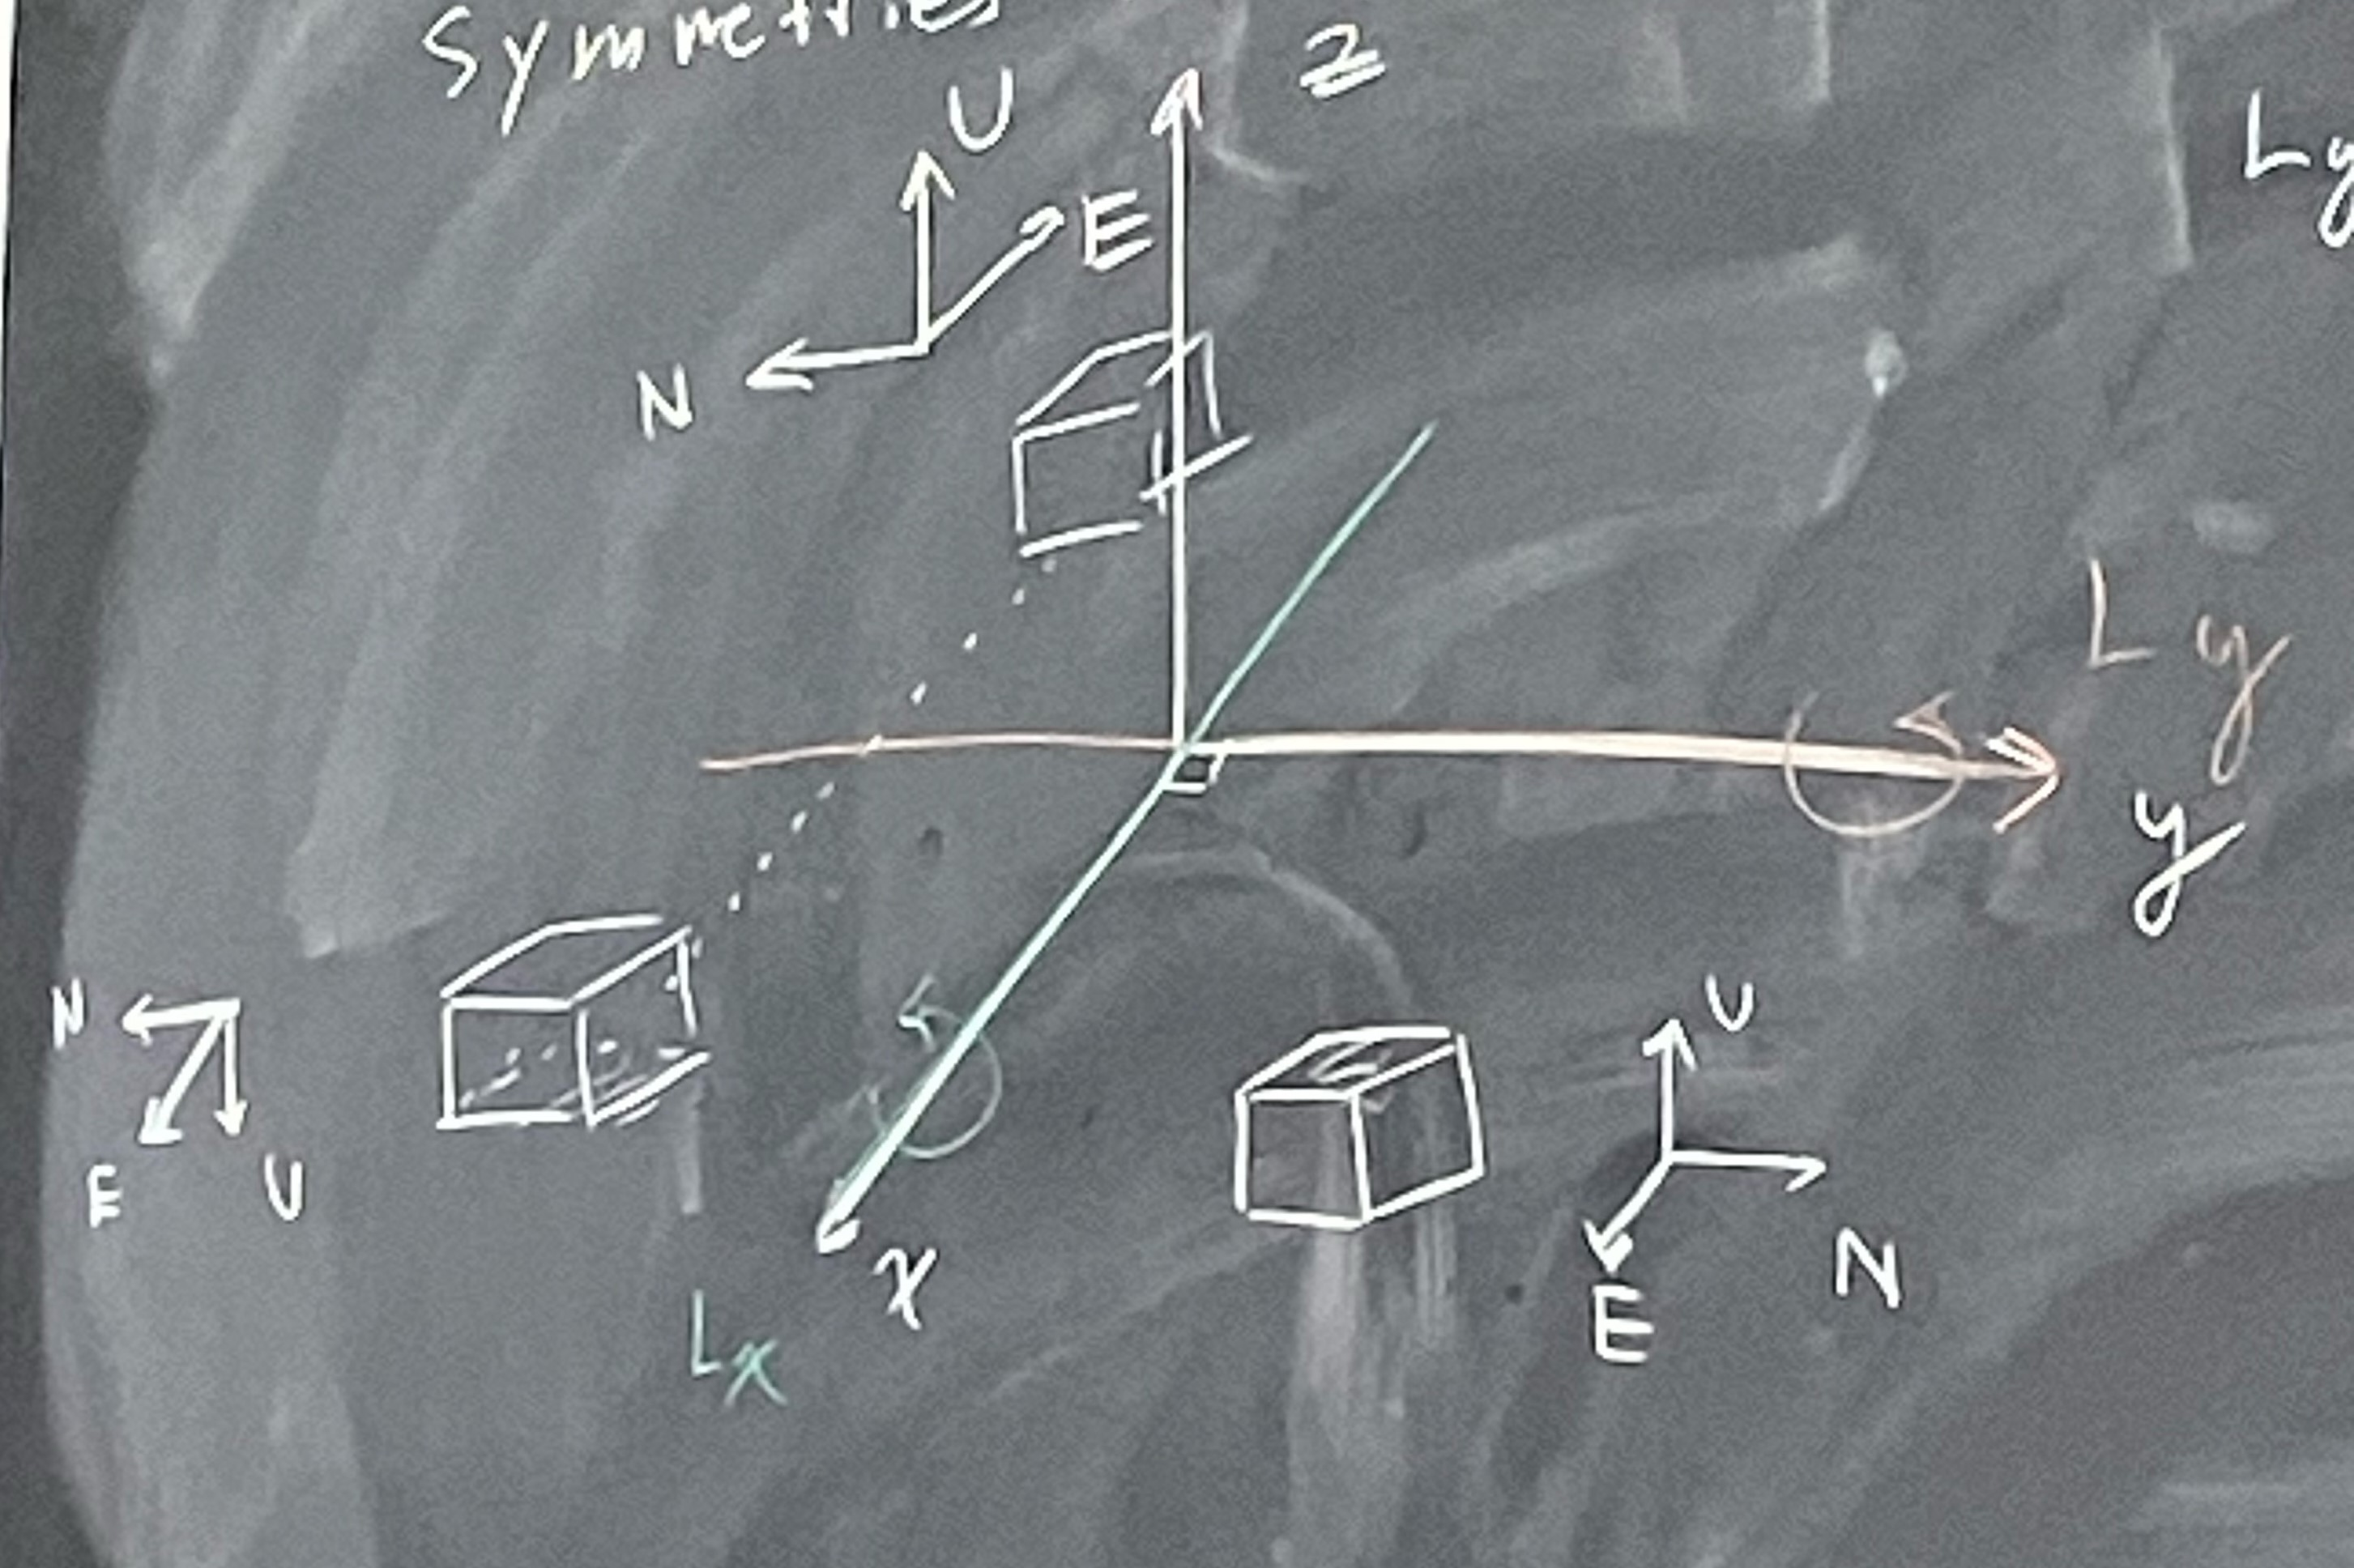
\includegraphics[width=0.8\textwidth]{Images/Cube symmetries.png}
    \end{center}

    We can express these in matrices in terms of the axes basis: 
    \[L_x = \begin{pmatrix}
        1\\ 
        & -1\\ 
        & & -1 
    \end{pmatrix}, \quad L_y = \begin{pmatrix}
        -1\\ 
        & 1\\ 
        & & -1
    \end{pmatrix}\]

    Clearly, $L_y \circ L_x$ is a composition of two rotations in $\SO(3, \R)$ so the result should also be a rotation. 

    From the diagram, we can see that $L_y \circ L_x$ should fix the $z$-axis and rotate orthogonal complement, i.e. $L_y L_x v = -v$. 

    Therefore, we could write $L_y \circ L_x = L_z$ in our basis. 

    What happens in the general case? 

    Let $A, B$ be lines in $\R^3$ through the origin. What is $L_B \circ L_A$ (where $L_A$ and $L_B$ denote the line symmetries of $A, B$ respectively). 

    One trivial case is if $L_A = L_B$ so $L_B \circ L_A = L_A^2 = 1_{\R^3}$.

    Now suppose $A \neq B$. Clearly, there is a non-zero angle between the two. 

    We can rotate the frame such that $L_A, L_B \subseteq $ the $xz$-plane. Since these are elements in $\SO(3, \R)$, we claim that a vector parallel to $A \times B$ is fixed by $L_B \circ L_A$: 
    \[(L_B \circ L_A)(A \times B) = L_B(L_A(A \times B)) = L_B(-A \times B) = A \times B\]
    So $A \times B$ is fixed by $L_B \circ L_A$.

    \begin{center}
        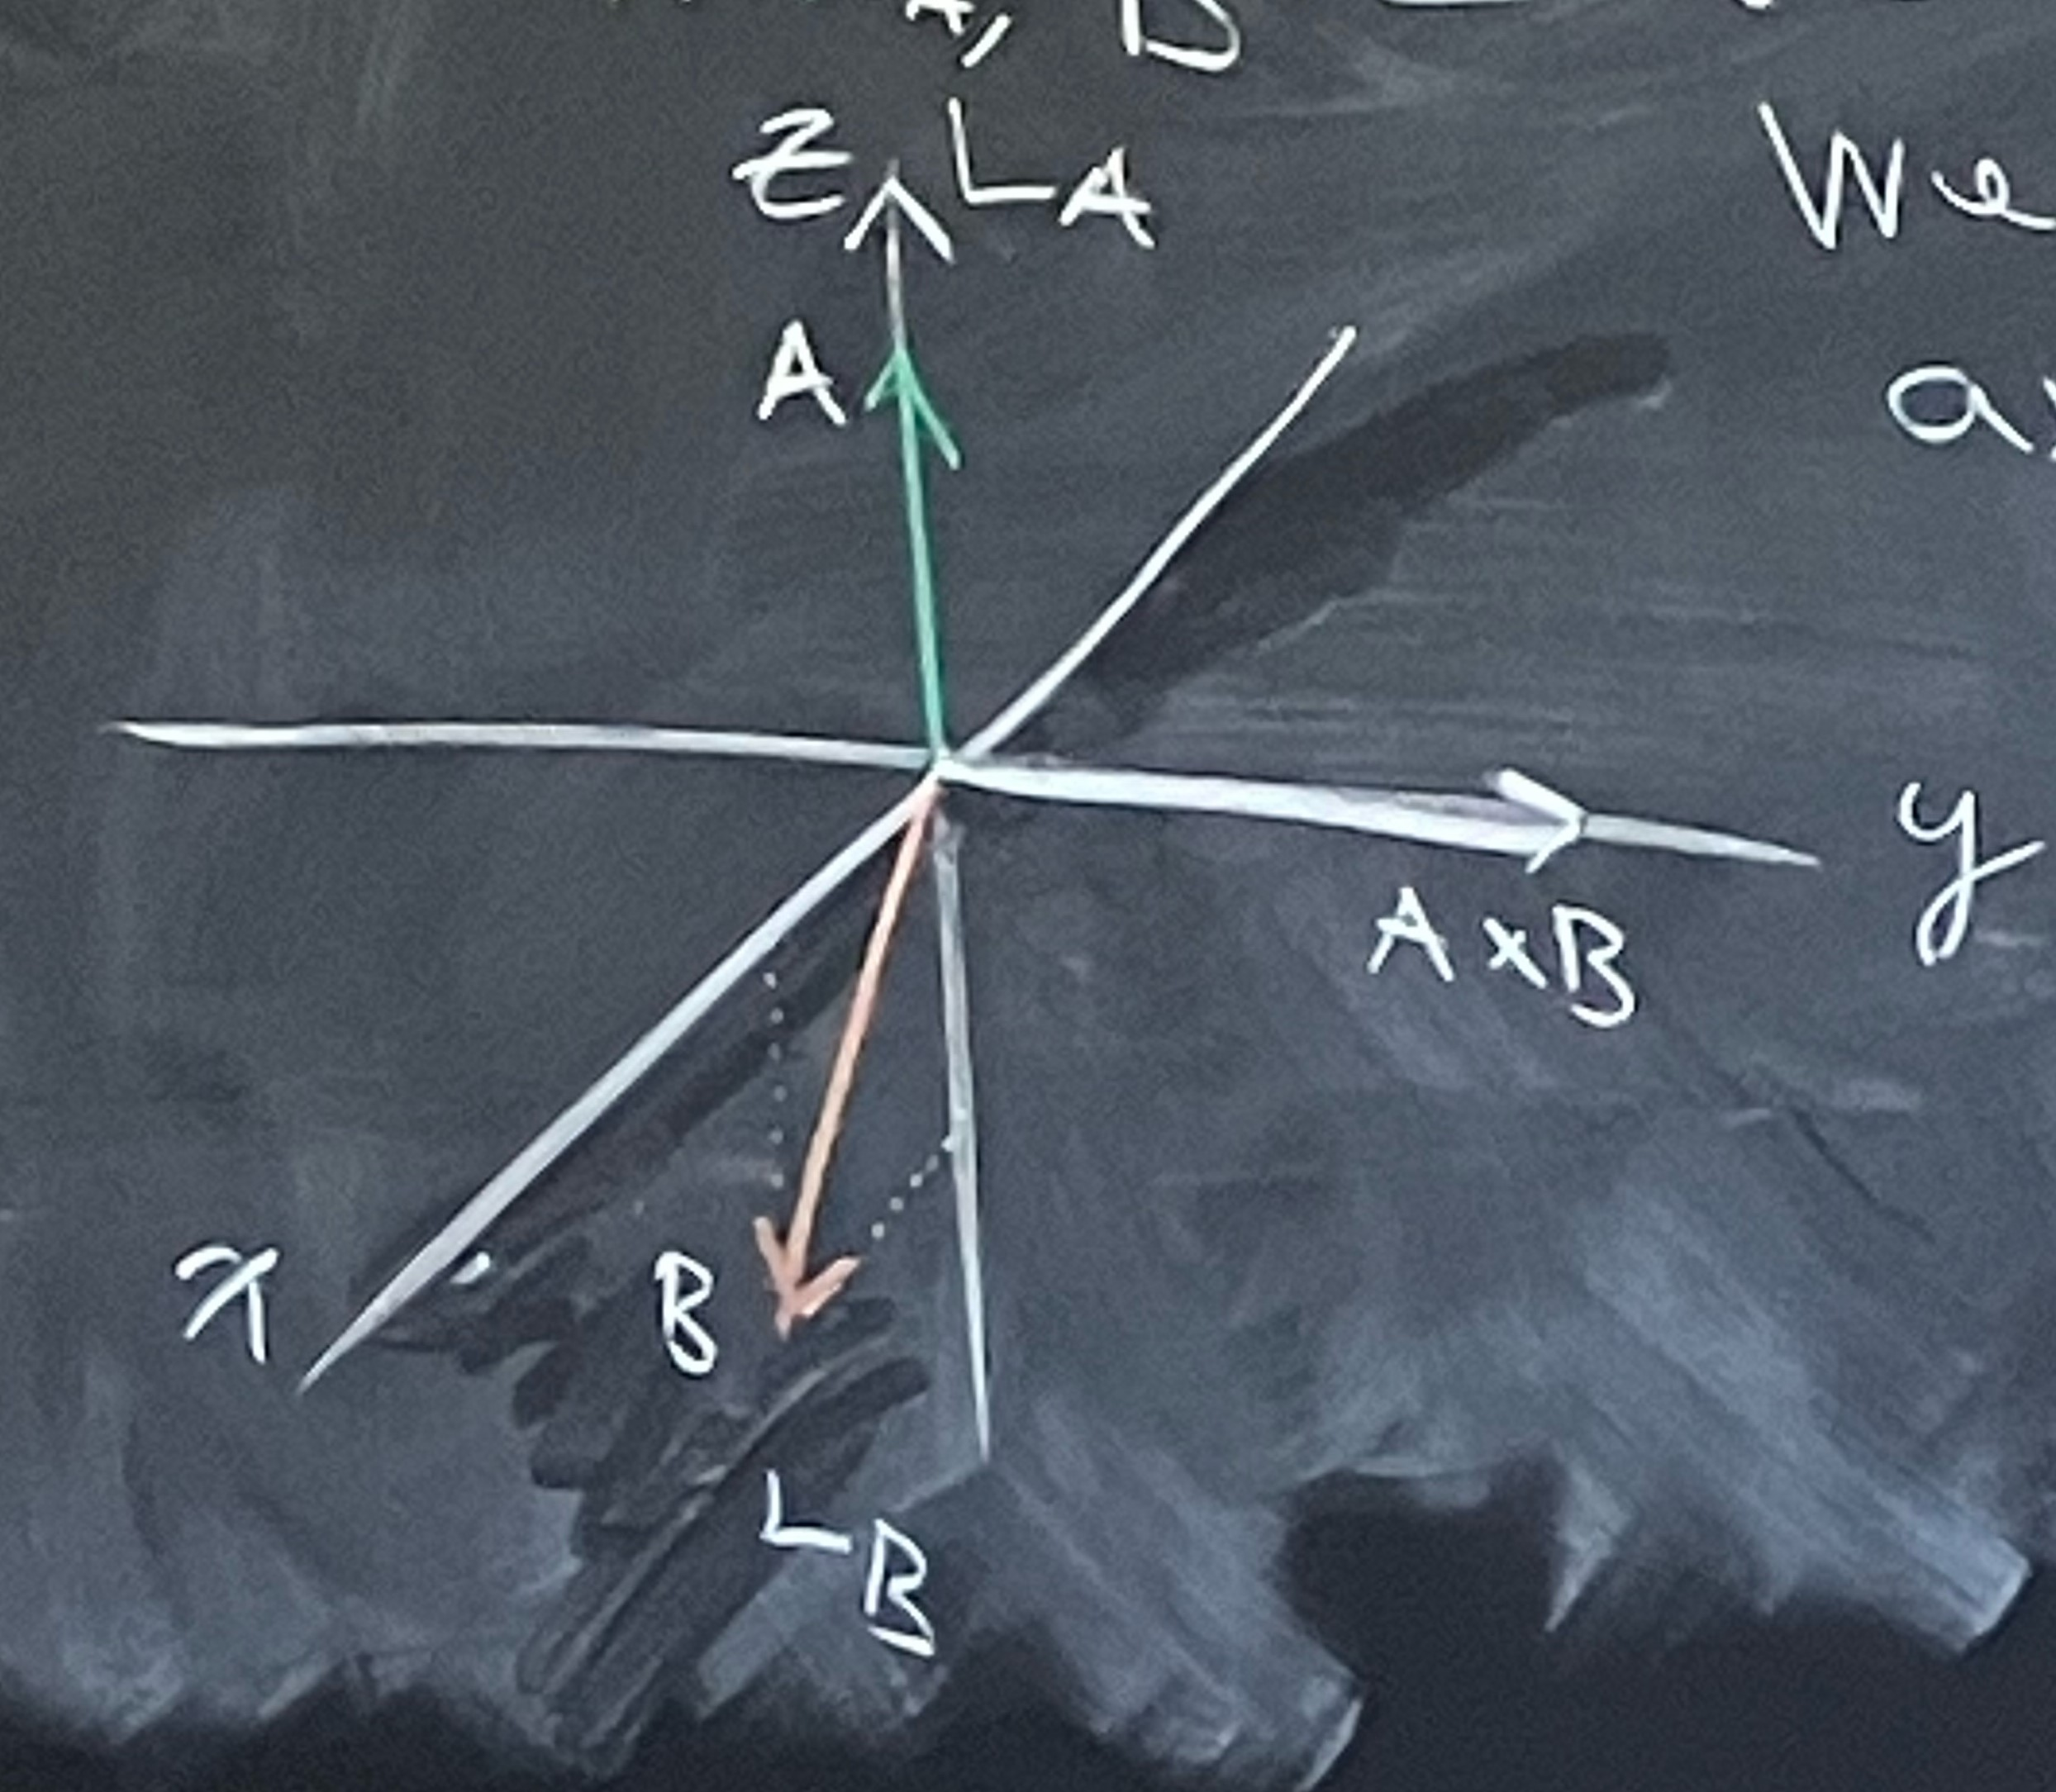
\includegraphics[width=0.8\textwidth]{Images/Fixed axis.png}
    \end{center}

    Because $A \times B$ is fixed by $L_B \circ L_A$, it suffices to determine what $L_B \circ L_A$ does on $\R(A \times B)^{\perp}$. 

    \begin{center}
        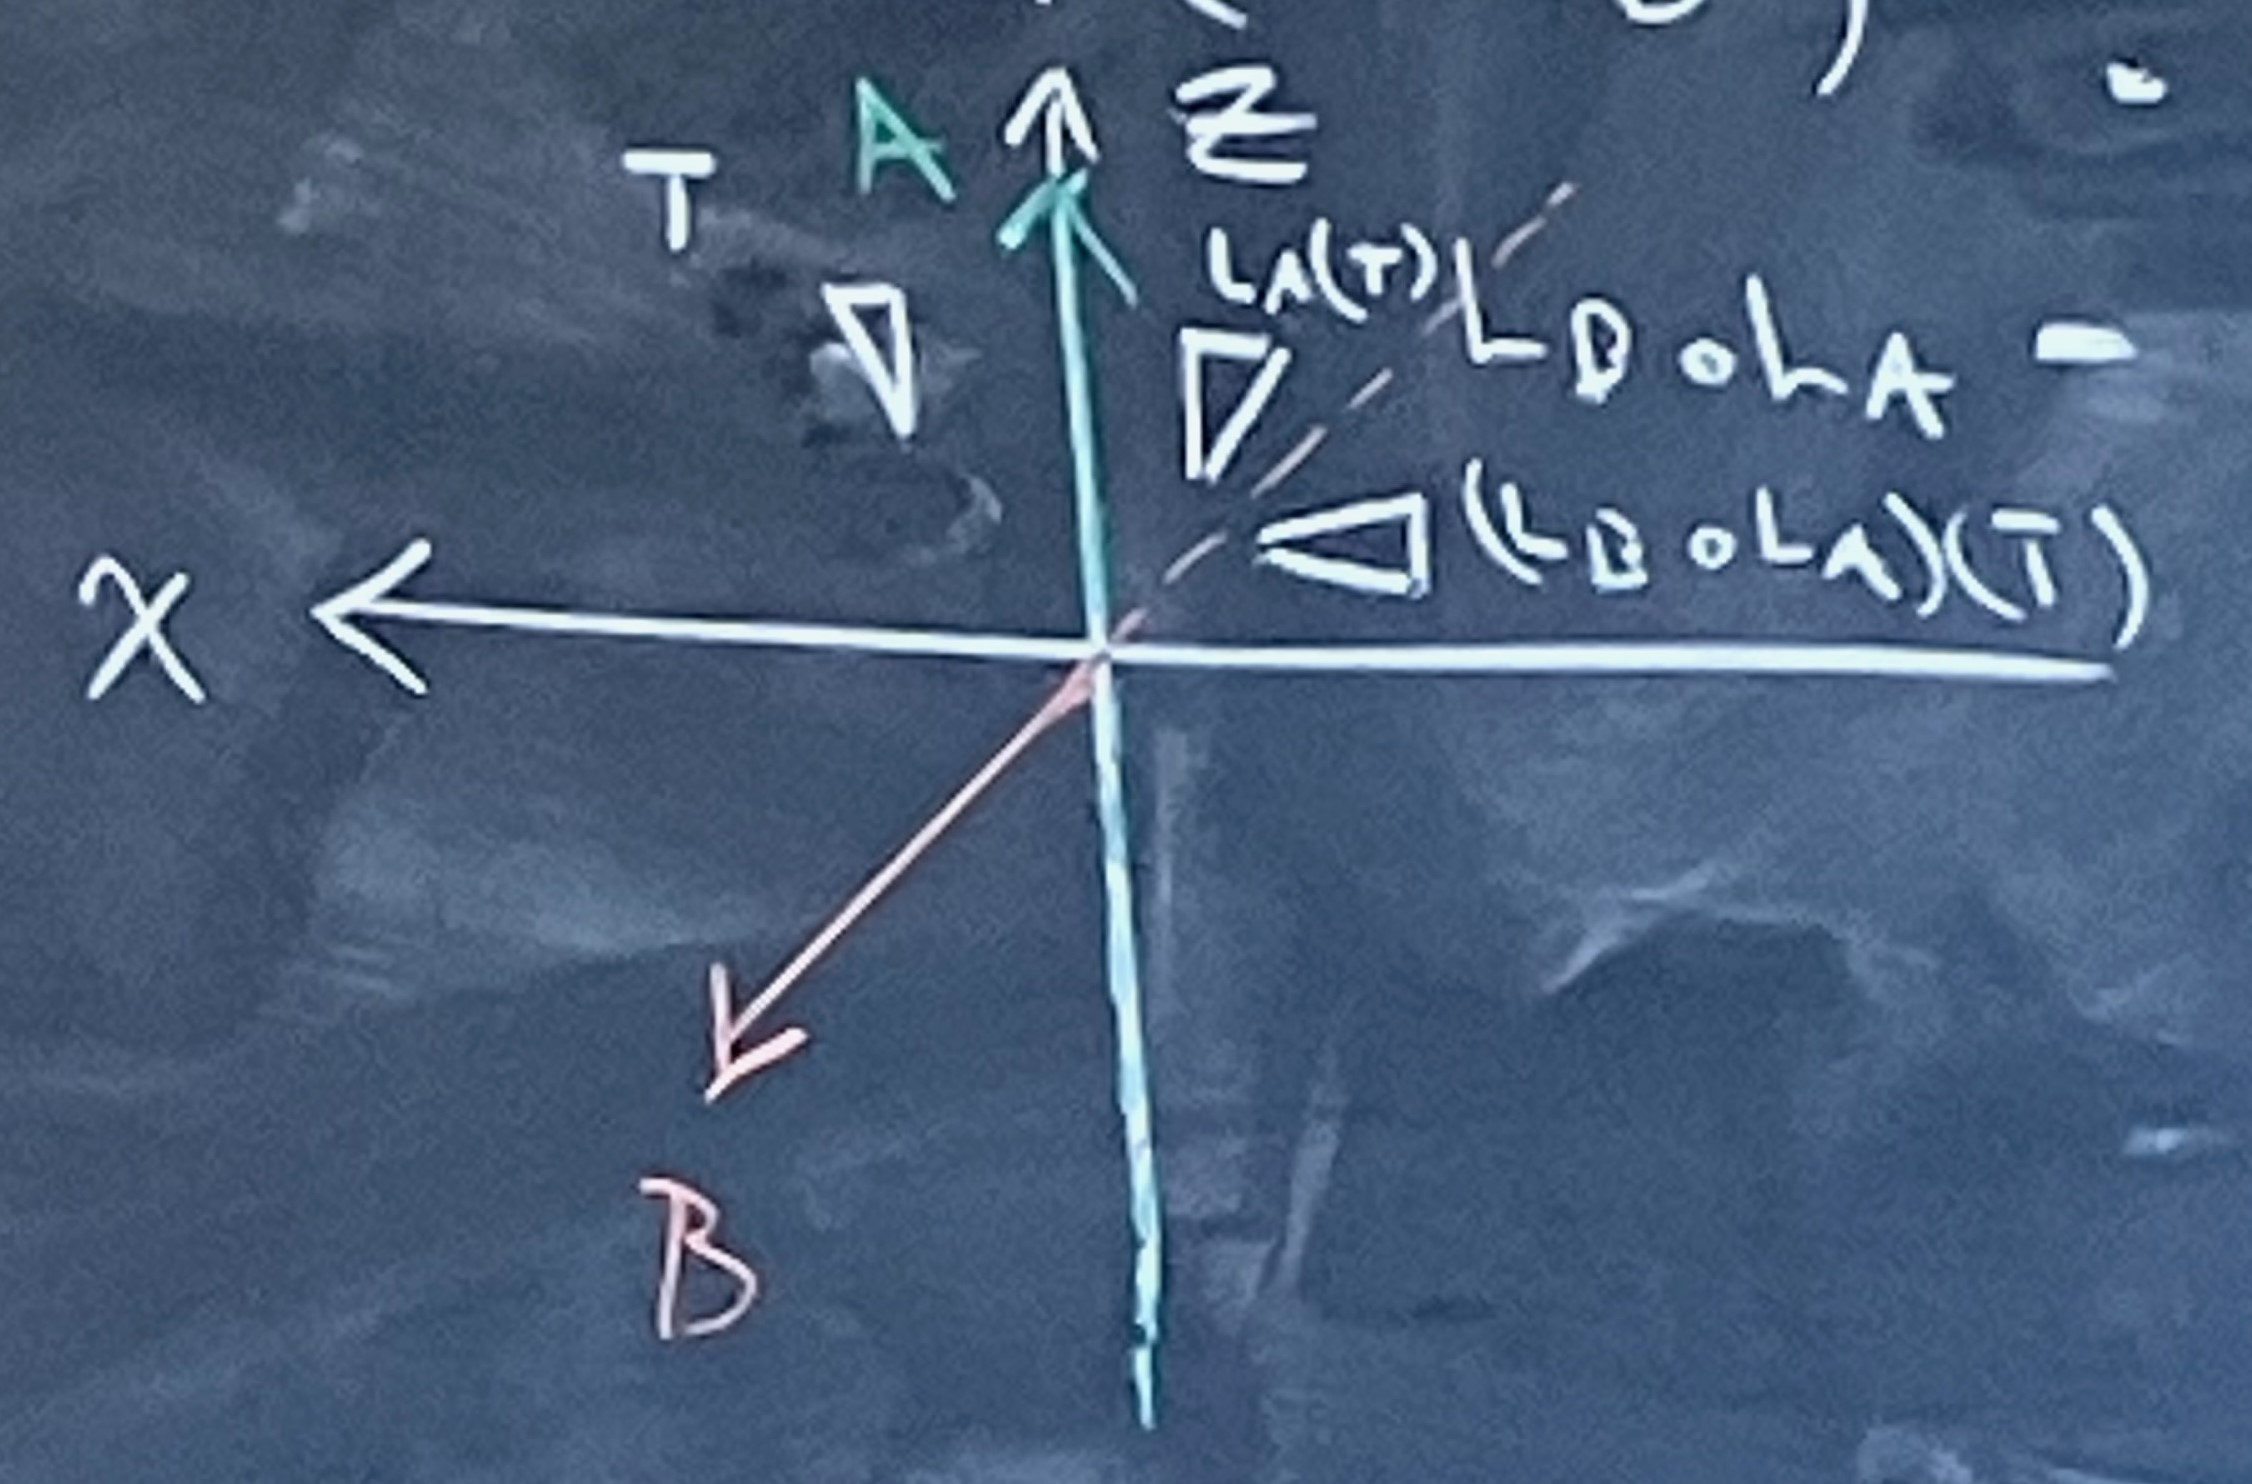
\includegraphics[width=0.8\textwidth]{Images/Triangle rotations.png}
    \end{center}


    And in fact this matches what we know from geometry: The composition of two line symmetries in the plane is a rotation by twice the angle from $A$ to $B$. 

    Therefore, $L_B \circ L_A$ fixes $A \times B$ and acts by a rotation of $2\theta$ from $A$ to $B$ where $\theta = \angle L_A, L_B$

    \begin{tbox}{\textbf{Euler-Rodrigues Theorem:} Let $q = \cos \frac{\theta}{2} + u \sin \frac{\theta}{2}$ be a unit quaternion in $S^3$. Then $I_q: P \biject P$ is a rotation about axis $u \in P$ by an angle of $\theta$}
        \emph{Proof:} Let $q = v^{-1}w$ where $v$ and $w$ are pure unit. We showed earlier that $q = vw_+ = w_- v$ so this is reasonable 

        Because $v, w \in P \cap S^3$, $q = (-v)w$. We therefore have 
        \[I_q = I_{-v} \circ I_w\]
        where $I_{-v}, I_w$ are line symmetries generated by $-v$ and $w$ respectively.

        From above, $I_q$ is thus a rotation about the plane perpendicular to $(-v) \times w$ by an angle of $2\phi$ (from $w$ to $-v$) so 
        \begin{align*}
            q &= (-v)w\\ 
            &= -(-v) \cdot w + (-v) \times w\\ 
            &= v \cdot w - v \times w\\ 
            &= \cos \phi + (-v \times w)\\ 
        \end{align*}
        (since $A \cdot B = \norm A\; \norm B\; \cos \psi$) 

        Here, the angle from $w$ to $v$ is $\phi$ and we know that 

    \end{tbox}

    \textbf{Consequence:} there exists a surjective lie group homomorphism $S^3 \twoheadrightarrow \SO(3, \R)$. 

    \emph{Proof:} Any non-trivial rotation in $\SO(3, \R)$ admits a fixed axis, and about $g$ , acts by rotating about a fixed axis by angle $\theta$. Surjectivity follows from Euler-Rodrigues. 

    However, this map is \emph{not} injective: Let $I_q$ act be the identity on $P$. Then $qvq^{-1} = v$
    for all $v \in P$. This suggests that $q \in Z(\H^{\times}) = \R^{\times}$ ($q$ commutes with all pure quaternions so it also commutes with all of $\H^{\times}$), so if $q$ is central (scalar) and unital, we know $q = \pm 1$. 

    Therefore, $\phi: S^3 \twoheadrightarrow \SO(3, \R)$ is surjective with kernel $\Z_2$. We call it the \emph{spin double cover} of $\SO(3, \R)$. 

    By the first isomorphism theorem, $S^3/\Z_2 \simeq \SO(3, \R)$. In a sense, $S^3/\Z_2$ is the topology on the space of all lines through $O$ in $\R^4$ denoted by $\RP^3$.
    
    Therefore,
    \[\RP^3 \simeq S^3/\Z_2 \simeq \SO(3, \R)\]

    In fact, we have another isomorphism. Notice that $\C^n$ is equipped with a bilinear form 
    \[\brak{\begin{pmatrix}
        z_1\\z_2\\ \vdots\\ z_n
    \end{pmatrix}, \begin{pmatrix}
        w_1\\w_2\\ \vdots\\ w_n
    \end{pmatrix}} = z_1 \bar{w_1} + z_2 \bar{w_2} + \dots + z_n \bar{w_n}\]
    with
    \begin{align*}
        \brak{cv, w} &= c\brak{v, w}\\ 
        \brak{v, cw} = \bar c\brak{v, w}
    \end{align*}

    In our case, $n = 2$. $\H$ is an $\R$-vector spaces (and in fact, it is an $\R$-algebra). Further, $\R$ sits in $\H$ centrally. 

    Additionally, $\H$ is a $\C$-vector space but \emph{not} a $\C$-algebra (intuition: $\C$ is not in $\R$) 

    This just means that we need to take some care. Let's construct $\H$ as a $\C$-vector space. What should $\C$-multiplication look like? A natural choice is to use the copies of $\C$ in $\H$ to get the desired representation of quaternion multiplication. 

    Let's choose $\beta = \{1, j\}$ as our $\C$-basis for $\H$ (as a complex vector space). That way, 
    \[a + b\ihat + c\jhat + d\khat = (a + bi)\cdot 1 + (c + di)\jhat\]

    Now we have to construct a representation for left-multiplication.

    First, a simpler example: $\C$ is an $\R$ vector space. $\beta = \{1, i\}$ is an $\R$-basis for $\C$. 
    \[L_{a + bi}: \quad \begin{aligned}
        \C &\to \C\\ 
        z &\mapsto (a + bi)c
    \end{aligned}\] 
    so $\C \simeq \R^2$. 

    \begin{align*}
        L_{a+bi}(1) &= a + bi\\ 
        L_{a+bi}(i) &= -b + ai
    \end{align*}
    so 
    \[({L_{a+bi}}_{\beta}) = \begin{pmatrix}
        a & b\\ 
        -b & a
    \end{pmatrix}\]

    Returning to the quaternions, we have $\H$ as a $\C$-space with basis $\beta =\{1, j\}$. We want 
    \begin{align*}
        L_{a + b\ihat + c\jhat + d\khat}(1) &= a + b\ihat + c\jhat + d\khat\\ 
        L_{a +bi + cj + dk}(j) &= aj + bk -c - di\\ 
            &= (-c - di) + (aj + bk)\\ 
            &= (-c - di)\cdot 1 + (a + bi)\jhat\\
    \end{align*}
    (note there is some notational subtlety: in the last line $1, j$ are the $C$-basis elements but $i, j, k$ above are the $\H$-basis) 
    so 
    \[(L_q)_{\beta} = \begin{pmatrix}
        a + bi & c + di\\ 
        -c - di & a + bi
    \end{pmatrix}\]
    which seems to make sense! 

    \emph{However}! This implies that $L_q(zp) = zL_q(p)$ for all $z \in \C$. Is this actually true? Consider:
    \[q(zp) \neq z(qp)\]
    so in fact, our derivation required assumptions of commutativity that we don't actually have! 
    
    There are two choices of $\C$ vector space on $\H$. We looked at the left action, but we really want $\H$ as a \emph{right} vector space!
 
\section{April 12:}
    Last time, we were considering $\H$ as a $\C$-vector space with 
    \[z = \begin{aligned}
        a + bi &\hookrightarrow \H\\ 
        a + bi &\mapsto a + b\ihat
    \end{aligned}\]
    so left multiplication extends naturally to yield a left $\C$-vector space of $\H$. 

    For each $q \in \H$ we get the map 
    \[L_q: {}^{\C} \H \biject {}^{\C}\H\]
    while the map is additive, it does \emph{not} preserve the vector space structure:
    \begin{align*}
        L_q(cp) &= cL_q(p) \quad \forall c\in \C, q, p\in \H\\ 
        q(cp) &= c(qp) 
    \end{align*}

    One solution is to consider $R_q$, the right action, instead. 
    \begin{align*}
        L_{qp}(h) &= (qp)h = q(ph) = (L_q \circ L_p)(h)\\ 
        L_{qp} &= L_q \circ L_p
    \end{align*} 
    \begin{align*}
        R_{qp}(h) &= (hq)p = R_p(h_q) = (R_p \circ R_q)(h)\\
        R_{qp} &= R_p \circ R_q
    \end{align*}
    So instead $\H^{\times} \to \Aut(\H)$ by $q \mapsto R_{q^[-1]}$

    However, this is still a little awkward. Therefore, let's consider $\H$ as a \emph{right} $\C$-vector space, $\H^{\C}$ instead of ${}^{\C}\H$.

    So $a + b\ihat + c\jhat + d\khat$ relative to the $\C$-basis $\beta = \{1, \jhat\}$ is 
    \[1 \cdot (a + bi) + \jhat(c - di)\] 
    (since $\jhat \ihat = -\khat$) and 
    \[L_q(pc) = q(pc) = (qp)c = L_q(p)c\]

    This way, for each $q \in \H$, $L_q$ is an honest $\C$-endomorphism of $\H^{\C}$ (a right $\C$-space)

    We want to see how $(L_q)_{\beta}$ looks in this context. Choosing a basis $\beta = \{1, \jhat\}$, 
    \[\begin{aligned}
        \H^{\times} \hookrightarrow \GL(\H^{\C}) \simeq \GL(2, \C)\\
        q &\mapsto L_q
    \end{aligned}\]
    so we can say 
    \[q = z + \jhat w \implies (q)_{\beta} = \begin{pmatrix}
        z \\ w
    \end{pmatrix}, \quad z, w \in \C\] 
    and 
    \begin{align*}
        L_q(1) &= z + \jhat w\\
        L_q(\jhat) &= q\jhat\\ 
            &= (z + \jhat w)\jhat\\ 
            &= z\jhat + \bar w + \jhat \jhat\\ 
            &= z \jhat - \bar w\\ 
            &= -\bar w + \jhat \bar z
    \end{align*}
    since 
    \[\jhat w = \jhat(a + b\ihat) = \jhat a + b\jhat \ihat = a\jhat - b \hat k = (a - b\hat i)\jhat\]
    which implies 
    \begin{align*}
        (L_q(1))_{\beta} &= \begin{pmatrix}
            z\\w
        \end{pmatrix}\\ 
        (L_q(\jhat))_{\beta} &= \begin{pmatrix}
            -w\\\bar z
        \end{pmatrix}
    \end{align*}
    so we have 
    \[(L_q)_{\beta} = \begin{pmatrix}
        z & -\bar w\\ 
        w & \bar z
    \end{pmatrix}\]

    Further, $\det L_q = z\bar z + w\bar w$ which gives us a representation of $\H^{\times} \hookrightarrow \GL(2, \C)$. The restriction onto elements of $\H^{\times}$ with $\norm{\cdot} = 1$ gives us the stronger representation 
    \[S^3 \hookrightarrow \SU(2, \C)\] 
    where $\SU(2, \C)$ is the group of $2 \times 2$ unitary matrices (matrices which preserve $\brak{z, w} = z_1 \bar w_1 + z_2 \bar w_2$ or equivalently, matrices with $A^{\dagger}A = (\bar A)^TA = I_2$) with determinant 1.

    Once you have 
    \[\SU(2, \C) = \left\{\begin{pmatrix}
        z & -\bar w\\ 
        w & \bar z
    \end{pmatrix} \bigg\vert z\bar z + w\bar w = 1\right\}\]
    then $S^3 \biject \SU(2, \C)$ and 
    \[\begin{tikzcd}
        S^3 \arrow[hook, two heads]{r}{\simeq} \arrow[two heads]{d}{\Z_2} & \SU(2, \C) \arrow[two heads]{dl}{\Z_2}\\
        \SO(3, \R) &
    \end{tikzcd}\]

    Now we turn to yet another similar representation, $S^3 \times S^3 \twoheadrightarrow \SO(4, \R)$ with a $\Z_2$-kernel. ($\text{Spin}(4, \R) \simeq S^3 \times S^3$) 

    Similar to the case of $\H$ as a $\C$-vector space, we can consider $\H$ as an $\R$-vector space (which means we do not have to worry about left/right structure). 

    With basis $\beta = \{1, \ihat, \jhat, \khat\}$, we can write
    \begin{align*}
        L_q &\sim \begin{pmatrix}
            x & -y & -z & -w\\ 
            y & x & -w & z\\
            z & w & x & -y\\
            w & -z & y & x
        \end{pmatrix}\\ 
        R_q &\sim \begin{pmatrix}
            x & -y & -z & -w\\ 
            y & x & w & -z\\
            z & -w & x & y\\
            w & z & -y & x
        \end{pmatrix}
    \end{align*}

    Notice! For each $q \in \H$ we get orthogonal columns so 
    \begin{align*}
        L_{\bar q} &\sim \begin{pmatrix}
            x & y & z & w\\ 
            -y & x & w & -z\\
            -z & -w & x & y\\
            -w & z & -y & x
        \end{pmatrix}
    \end{align*}
    so $L_{\bar q} = (L_q)^T$ and $L_{q\,\bar q} = q\,\bar qI_4$ since $q\, \bar q = \norm{q}^2 \in \R$. 

    Therefore, if $\norm{q} = 1$, we have $L{\bar q\, q} = L_{\bar q} L_q = L_q^T L_q = I_4$. So all $q \in \H^{\times}$ with $\norm{q} = 1$ have $L_q \in \SO(4, \R)$. 

    An analogous statement holds for $R_q$., 

    Note that for each $(p, q) \in S^3 \times S^3$, we get an element of $\SO(4, \R)$ so 
    \[(q, p) \mapsto \begin{aligned}
        \H \biject \H\\ 
        h \mapsto qhp = L_q \circ R_p
    \end{aligned}\]

    We want this to be a representation (homomorphism) so it suffices to take 
    \[(q, p) \mapsto L_q R_{p^{-1}} = R_{p^{-1}} L_q\] 

\section{April 15:}
    Last time, we noted that $q \mapsto (L_q)_{\beta}$ $(\beta = \{1, \ihat, \jhat, \khat\}$) gives us a faithful representation of $\H^{\times}$ in $\text{Sim}(4, \R)$. When $\norm{q} = 1$, we get $(L_q)_{\beta} \in \SO(4, \R)$. 

    We also saw the same thing for $R_{p^{-1}}$ relative to $\beta$: We have a homomorphism 
    \[\begin{aligned}
        S^3 \times S^3 &\to \SO(4, \R)\\ 
        (q, p) &\mapsto (L_q \circ R_{p^{-1}})_{\beta}
    \end{aligned}\]

    \begin{tbox}{\textbf{Claim:} This homomorphism is onto $\SO(4, \R)$}
        \emph{Proof:} We know that if $g \in \SO(4, \R)$ for which $g(1) = 1$ (letting $\R^4 \simeq \H$).

        We claim we can find $(p, q) \in S^3 \times S^3$ for which $L_p \circ R_{q^{-1}} = g$ such that $g: \H \biject \H$ and $g(1) = 1$. 

        In particular, this would induce a map on $(\R 1)^{\perp} = P$ (the pure Hamiltonians) so we have 
        \[g\big\vert_p: P \biject P\]
        such that 
        \[(q, p)\in S^3 \times S^3, \quad (L_q \circ R_{p^{-1}})\big\vert_P = g\big\vert_P\]

        But in fact, we already did this! Just look at the conjugation map $(L_q \circ R_{q^{-1}})(h) = qhq^{-1}$. We already showed this is acting as an element of $\SO(3, \R)$ and Euler-Rodrigues claims this is sujective. 

        Thus, if $g(1) = 1$, we can find $(p, q) \in S^3 \times S^3$ for which $L_q \circ R_{p^{-1}} = g$ and we are done. 

        However, it is also possible for $g(1) = p$. In this case, we can consider the composition:
        \[\psi = \phi_{(p^{-1}, 1)} \circ g\]
        where $\psi: S^3 \times S^3 \to \SO(4, \R)$. 

        \textbf{Note:} $\psi(1) = \phi_{(p^{-1}, 1)}(p) = p^{-1}p1^{-1} = 1$ so $\psi(1) = 1 \in \SO(4, \R)$.  
        
        By the first case, we can thus find $(p', q')$ so that $\phi_{(p', q')} = \psi = \phi_{(p^{-1}, 1)} \circ g$. 

        Thus $\phi: S^3 \times S^3 \to \SO(4, \R)$ is surjective. 

        We don't quite have injectivity but we do know that $\phi: S^3 \times S^3 \twoheadrightarrow \SO(4, \R)$ has a kernel of $\Z_2$ (precisely, $\ker \phi = \{(1, 1), (-1, -1)\}$. \emph{Proof:} HW). 

        This also tells us $S^3 \times S^3/\Z_2 \simeq \SO(4, \R)$, which means $S^3 \times S^3$ is a double cover of $\SO(4, \R)$. So we say $S^3 \times S^3 \simeq \text{Spin}(4, \R)$. 
    \end{tbox}

    \textbf{Definition:} A \emph{Fibre Bundle} is a (surjective) smooth map 
    \[E \overset{p}{\twoheadrightarrow} B\]
    from a total space $E$ to a base $B$ such that for a small set $U \subseteq B$, $p^{-1}(U) \simeq U \times F$. 

    A \emph{fibre} is the inverse-image/pull-back of a point under a map 

    Heuristically, this is a parameterization of $E$ over a variable $B$. 

    \textbf{Example:}
    \[\begin{aligned}
        \R^2 &\twoheadrightarrow \R\\ 
        (x, y) &\mapsto x
    \end{aligned}\]
    is an $\R$-bundle. 

    \begin{center}
        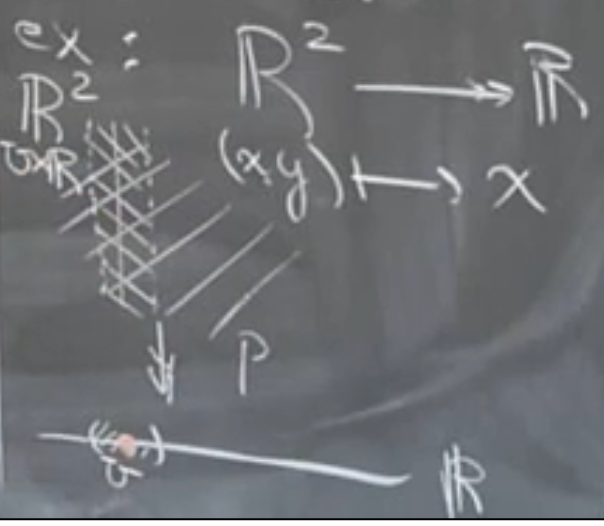
\includegraphics[width=0.8\textwidth]{Images/April 16 - R2 bundle.png}
    \end{center}

    Clearly this projects the entire plane onto the real line. Given a point, if we consider its fibre, we get the vertical line corresponding to $x = p$. If we take a neighborhood $U$ around the point, then the neighborhood around the fibre will indeed look like $U \times \R$. 

    \textbf{Example:} Now consider a cylinder ($E$) projected onto its base ($B = S^1$).
    
    Since $p^{-1}(U) \simeq U \times I$, $I = [0, 1]$ so we say $E$ is an $I$-bundle over $S^1$

    \begin{center}
        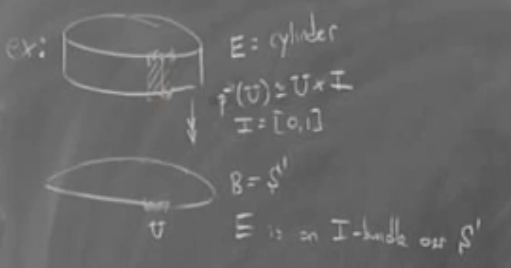
\includegraphics[width=0.8\textwidth]{Images/April 16 - Cylinder bundle.png}
    \end{center}

    \textbf{Example:} With $E$ a Mobius band, we can also consider $E$ as a $I$-bundle over $S^1$.

    \begin{center}
        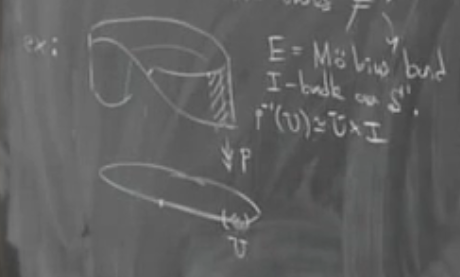
\includegraphics[width=0.8\textwidth]{Images/April 16 - Mobius bundle.png}
    \end{center}

    However, these two bundles are different! The Mobius band is orientable but the cylinder is not. 

    \textbf{Example:} We can do the same thing with a torus! 

    \begin{center}
        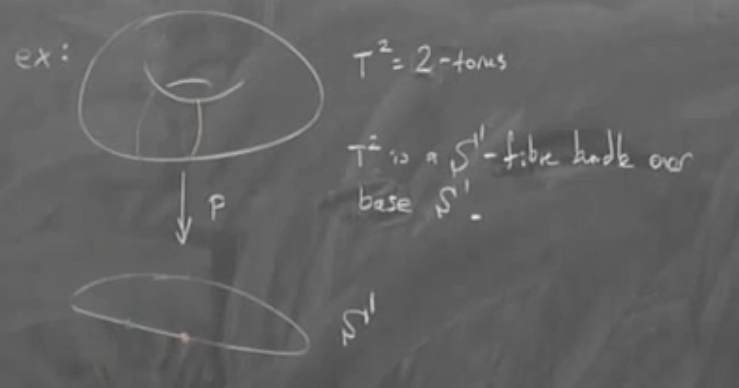
\includegraphics[width=0.8\textwidth]{Images/April 16 - Torus bundle.png}
    \end{center}

    Notice that we are taking circles to points on $S^1$ so the 2-torus, $T^2$, is a $S^1$-fibre bundle over base $S^1$.

    And further, it remains so up local deformations: 
    \begin{center}
        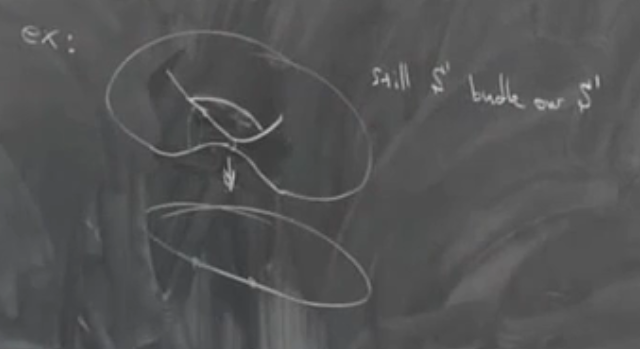
\includegraphics[width=0.8\textwidth]{Images/April 16 - Pinched torus bundle.png}
    \end{center}
    is still an $S^1$-bundle over $S^1$.

    But 
    \begin{center}
        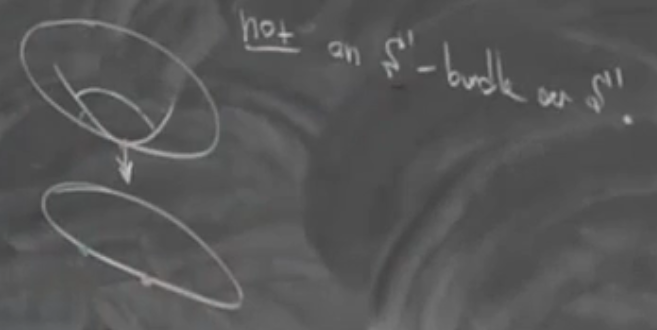
\includegraphics[width=0.8\textwidth]{Images/April 16 - Deformed torus bundle.png}
    \end{center}
    is \emph{not}, because one of the fibres is a point -- not a circle. 

    \textbf{Example:} We can also consider cut-and-paste constructions. 

    If we take the original torus and cut along the red circle and down the center, we can construct this square: 
    \begin{center}
        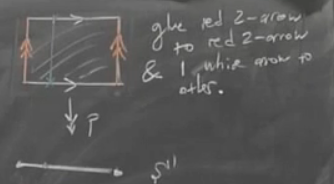
\includegraphics[width=0.8\textwidth]{Images/April 16 - Torus square.png}
    \end{center}
    (Note: gluing red 2-arrow to red 2-arrow and white 1-arrow to white 1-arrow reconstructs the torus)

    Notice that arrow orientation matters! If we instead consider this bundle: 
    \begin{center}
        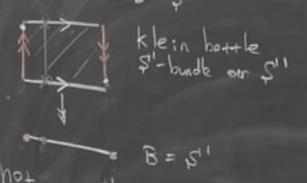
\includegraphics[width=0.8\textwidth]{Images/April 16 - Klein square.png}
    \end{center}
    we get a Klein bottle $S^1$-bundle over $S^1$, not a torus! 

    \subsection*{The Hopf-Fibration}
    \textbf{Hopf-Fibration (Fibre bundle):} an $S^1$-bundle over $S^2$ base on total space $S^3$. 

    Put differently, we have $p: S^3 \twoheadrightarrow S^2$ such that $p^{-1}\{h\} \simeq S^1$

    \textbf{Motivation:} Recall the Stereographic projection that lets us write 
    \begin{align*}
        S^1/N &\simeq \R\\ 
        S^2/N &\simeq \R^2\\
        S^3/N &\simeq \R^3
    \end{align*}

    Question: Is there a way to decompose $\R^3$ into disjoint circles and 1-line? 

    Here is one way: 
    \begin{center}
        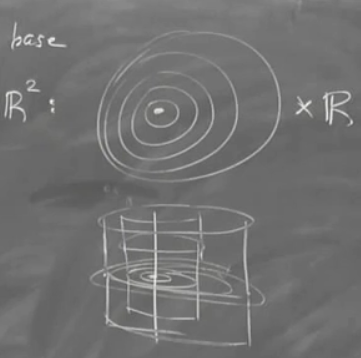
\includegraphics[width=0.8\textwidth]{Images/April 16 - Disjoint circles.png}  
    \end{center}
    
    Harder Question: Can we decompose $\R^3$ into disjoint circles and one line so that all circles and lines are linked? (linked in the sense of interlocked rings)

    We can visualize this slightly more easily via the Stereographic projection $f: S^2/N \biject \R^2$

    \begin{center}
        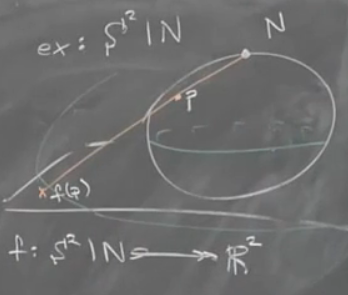
\includegraphics[width=0.8\textwidth]{Images/April 16 - Stereographic.png}
    \end{center}

\section{April 17:}
    Recall a fibre bundle is a sequence of homomorphisms 
    \[F \hookrightarrow E \overset{p}{\twoheadrightarrow} B\] 
    where $E$ is a total space, $B$ is a base space, and $F$ is a fibre ($p^{-1}\{b\} = F$)

    The typical example is a torus projecting onto $S^1$ such that the cross sections are themselves circles (locally look like $S^1$). 

    Further, this is a \emph{local} condition in the sense that a neighborhood $U(b)$ with $b \in B$ has pre-image $p^{-1}(U) = U \times F$ 

    The \emph{Hopf-fibration} is a circle ($S^1$) bundle over $S^2$. Precisely, it is a \emph{principal G-bundle}, a fibre bundle equipped with a right $G$-action on the total space so that the fibres are ``equal'' to $G$. 

    \emph{Example:} A subset of $\R^2$ projecting down into an interval $I \subset \R$ is one simple exacmple.

    \begin{center}
        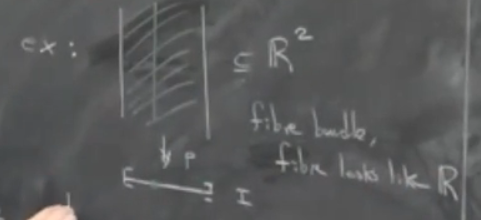
\includegraphics[width=0.8\textwidth]{Images/April 17 - R2 Hopf}
    \end{center}

    Certainly this is a fibre bundle. And in fact, we could write this out explicitly:
    \[E = \{(x, y) \; | \; 0 \leq x \leq 1, y \in \R\} \overset{p}{\twoheadrightarrow} I = [0, 1]\]
    so each of the fibres looks like $\R$. 

    We can define a right $\R$-action on $E$, $(x, y)t = (x, y + x)$ (an upwards translation along the fibre). 

    This allows us to say that the fibres are in fact isomorphic to $\R = G$. 

    \textbf{Example:} $T^2 = \{(\theta, \phi) \; | \; \theta, \phi \in \R/\Z\}$

    \begin{center}
        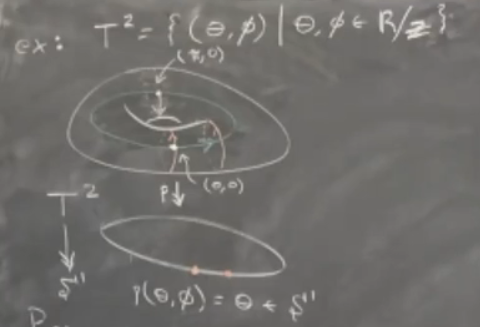
\includegraphics[width=0.8\textwidth]{Images/April 17 - T2} 
    \end{center}

    So we have $p: T^2 \twoheadrightarrow S^1$ by $p(\theta, \phi) = \theta \in S^1$. 

    In fact, this is a \emph{principal $S^1$-bundle}. 
    \[(\theta, \phi)t = (\theta, \phi + t), \quad t \in \R/\Z\]

    \begin{center}
        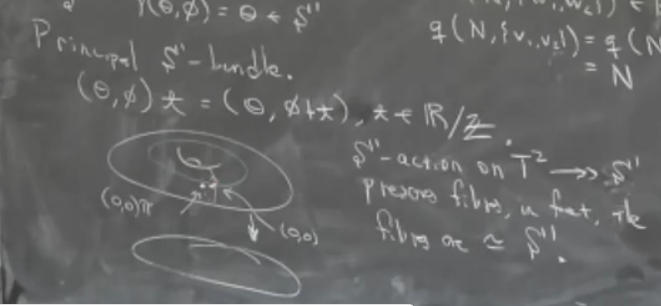
\includegraphics[width=0.8\textwidth]{Images/April 17 - T2 principal S1}
    \end{center}

    So this is an $S^1$-action on $T^2 \twoheadrightarrow S^1$ which preserves fibres. In fact, the fibres are isomorphic to $S^1$! 

    \textbf{Non-commutative example:} Let $M = S^2$. Consider 
    \[E = \{(p, \{v_1, v_2\}) \; | \; p \in S^2, \; v_1, v_2 \in T_p S^2 \text{ such that } T_p S^2 = \text{Span}\{v_1, v_2\}\}\] 
    with action $q(p, \{v_1, v_2\}) = p$. 

    We can visualize this by choosing $N \in S^2$. Then the tangent space $T_NS^2$ is just the plane tangent to $S^2$ at $N$ and we can choose any (linearly independent) vectors $v_1, v_2$ in this plane. So $(N, \{v_1, v_2\}) \in E$. 


    \begin{center}
        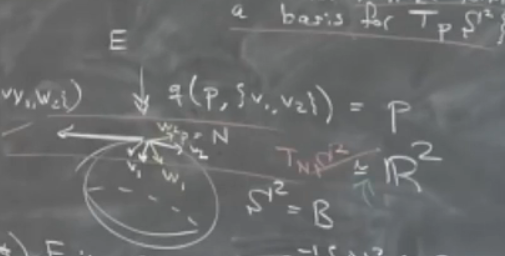
\includegraphics[width=0.8\textwidth]{Images/April 17 - Noncommutative manifold}
    \end{center}

    How do we choose another point in $E$? Just choose two more vectors in $T_{N}S^2$, say by rotation so we have $(N, \{w_1, w_2\}) \in E$ since 
    \[q(N, \{v_1, v_2\}) = q(N, \{w_1, w_2\}) = N\]
    
    For example: 
    \[\{v_1, v_2\} \begin{pmatrix}
        2 & 0\\ 
        0 & 1
    \end{pmatrix} \mapsto \{2v_1, v_2\}\] 

    Thus, we can say $E$ is a $\GL(2, \R)$ bundle over $S^2$. Our group action is $q^{-1}\{N\} \simeq \GL(2, \R)$ because we just need a choice of 2-vectors in $T_N S^2 \simeq \R^2$ that are linearly independent. 

    \textbf{Conclusion:} a \emph{principal $G$-bundle} is a fibre bundle $E$ with fibre $G$ such that the fibre is isomorphic to $G$ as a group 

    \textbf{Definition:} The \emph{Hopf-fibration} is a principal $S^1$ bundle over $S^2$ with total space $S^3$. 

    Recall: By Euler-Rodrigues, we have
    \[\begin{aligned}
        S^3 \twoheadrightarrow \SO(3, \R)\\ 
        q &\mapsto \begin{array}{c}
            I_q: P \biject P\\ 
            I_q(h) = qhq^{-1}
        \end{array}
    \end{aligned}\] 
    (where $P$ is the pure quaternion) 

    In particular, each $I_q$ preserves $S^2 = \{a \ihat + b\jhat + c\khat \; | \; a^2 + b^2 + c^2 = 1\}$, the pure quaternions with unit norm. 

    Claim: this yields a transitive $S^3$ action on $S^2$ via 
    \[\begin{aligned}
        S^3 &\to \Aut(S^2)\\ 
        q &\mapsto I_q: S^2 \biject S^2
    \end{aligned}\]
    which acts transitively because $\SO(3, \R)$ acts transitively on $S^2$ 

    Consequently, we have $H: S^3 \twoheadrightarrow S^2$ via $q \mapsto I_q(\khat)$: Because the action is transitive $\text{Orbit}(\khat) = S^2$. This map is precisely the Hopf fibration!

    Consider:  
    \[H(q) = H(a, b, c, d) = 2(ac + bd)\ihat - 2(ab + cd)\jhat + (a^2 - b^2 - c^2 + d^2)\khat\]

    By the orbit stabilizer theorem, $S^3/\text{Stab}(\khat) \simeq \text{Orbit}(\khat) \simeq S^2$. Therefore, we just need to find the stabilizer of $\khat$ since $S^3/\text{Stab}(\khat) \simeq S^2$. 

    We know $\text{Stab}(\khat) = \{q \in S^3 \; | \; I_q(\khat) = \khat\} = \{q \in S^3 \; | \; q\khat q^{-1} = \khat\}$. 

    Certainly, we know $q\khat q^{-1} = \khat$ for the plane generated by $\{1, \khat\} \simeq \C$ ($\khat$ will commute with the scalars and with itself). Then, it suffices to show that $\khat$ does \emph{not} commute with elements of the plane $\{\ihat, \jhat\}$ (Exercise). 

    Therefore, $\text{Stab}(\khat)= \{\cos\theta + \sin\theta \khat \; | \; \theta \in \R\} \simeq S^1$. 

    So 
    \[S^3/S^1 \simeq S^2\]

\section{April 22:}
    \textbf{Recall:} The \emph{Hobf-Fibration} is a surjective map $H: S^3 \twoheadrightarrow S^2$ defined by $q \mapsto q\khat q^{-1}$. 

    Last time, we found a fibre over $\khat = \{q \in S^3 \; | \; H(q) = q\khat q^{-1} = \khat\} = \text{Stab}(\khat)$ when $S^3$ acts on itself via conjugation. 
    
    The argument: the plane generated by $\text{Span}_{\R}\{1, \khat\} \in \H^{\times}$ is preserved by conjugation. 

    Geometrically, when we take this plane minus $0$ and normalize, we have the circle $S^1$. 

    Therefore, a nice parameterization is given 
    \[\text{Stab}(\khat) = \{\cos \theta + \khat \sin \theta \; | \; \theta \in [0, 2\pi]\}\]

    A \emph{Principal $G$-bundle} is a fibre bundle $E \twoheadrightarrow B$ with fibre $F$ where $F \simeq G$ as a group. Equivalently, we have a right $G$-action on $E$ that preserves fibres where the fibres are isomorphic to $G$.

    \begin{tbox}{\textbf{Claim:} The Hopf fibration $H: S^3 \to S^2$ is a principal $S^1$-bundle over $S^2$}
        \emph{Proof:} Let $q \in S^3$ so that $H(q) = v \in S^2$. (Geometrically, $q$ projects down to $v$ on the sphere)

        How do we get the $S^1$-action? We can consider rotations. Note with $s \in S^1$,
        \[H(qs) = qs\khat (qs)^{-1} = qs\khat s^{-1}q^{-1} = q\khat q^{-1} = H(q)\] 
        which confirms we have a right $S^1$ action that preserves the fibres of $S^3 \twoheadrightarrow S^2$
    \end{tbox}

    Note: that there exists a non-zero vector field $X$ on $S^3$ is not surprising. (How could we get an arbitrary vector field on $S^3$? Just choose a non-zero $v \in T_1 S^{3}$ so we have an $S^3$ action by left multplication.) Indeed, you can do this for any Lie group - the tangent bundle is parallelizable! 

    What happens with left multiplication in the Hopf-fibration? 
    \[H(qp) = qp\khat (qp^{-1}) = qp\khat p^{-1}q^{-1} = qH(p)q^{-1} = I_q(H(p))\]
    is just rotation of $H(p)$ about the vector part of $q$. 

    This tells us how to find the fibre over a specific point in $S^2$ -- it is just a geometric problem:

    We want to find $H^{-1}\{v\}$ with $v \in S^2$. But if we find \emph{any} $v \in S^3$ with $H(q) = v$, then we have the full fibre since $H^{-1}\{v\} = qS$ where $S = \text{Stab}(\khat)$. 

    Thus, we are searching for a single $q \in S^3$ where $H(q) = v$. 

    \begin{center}
        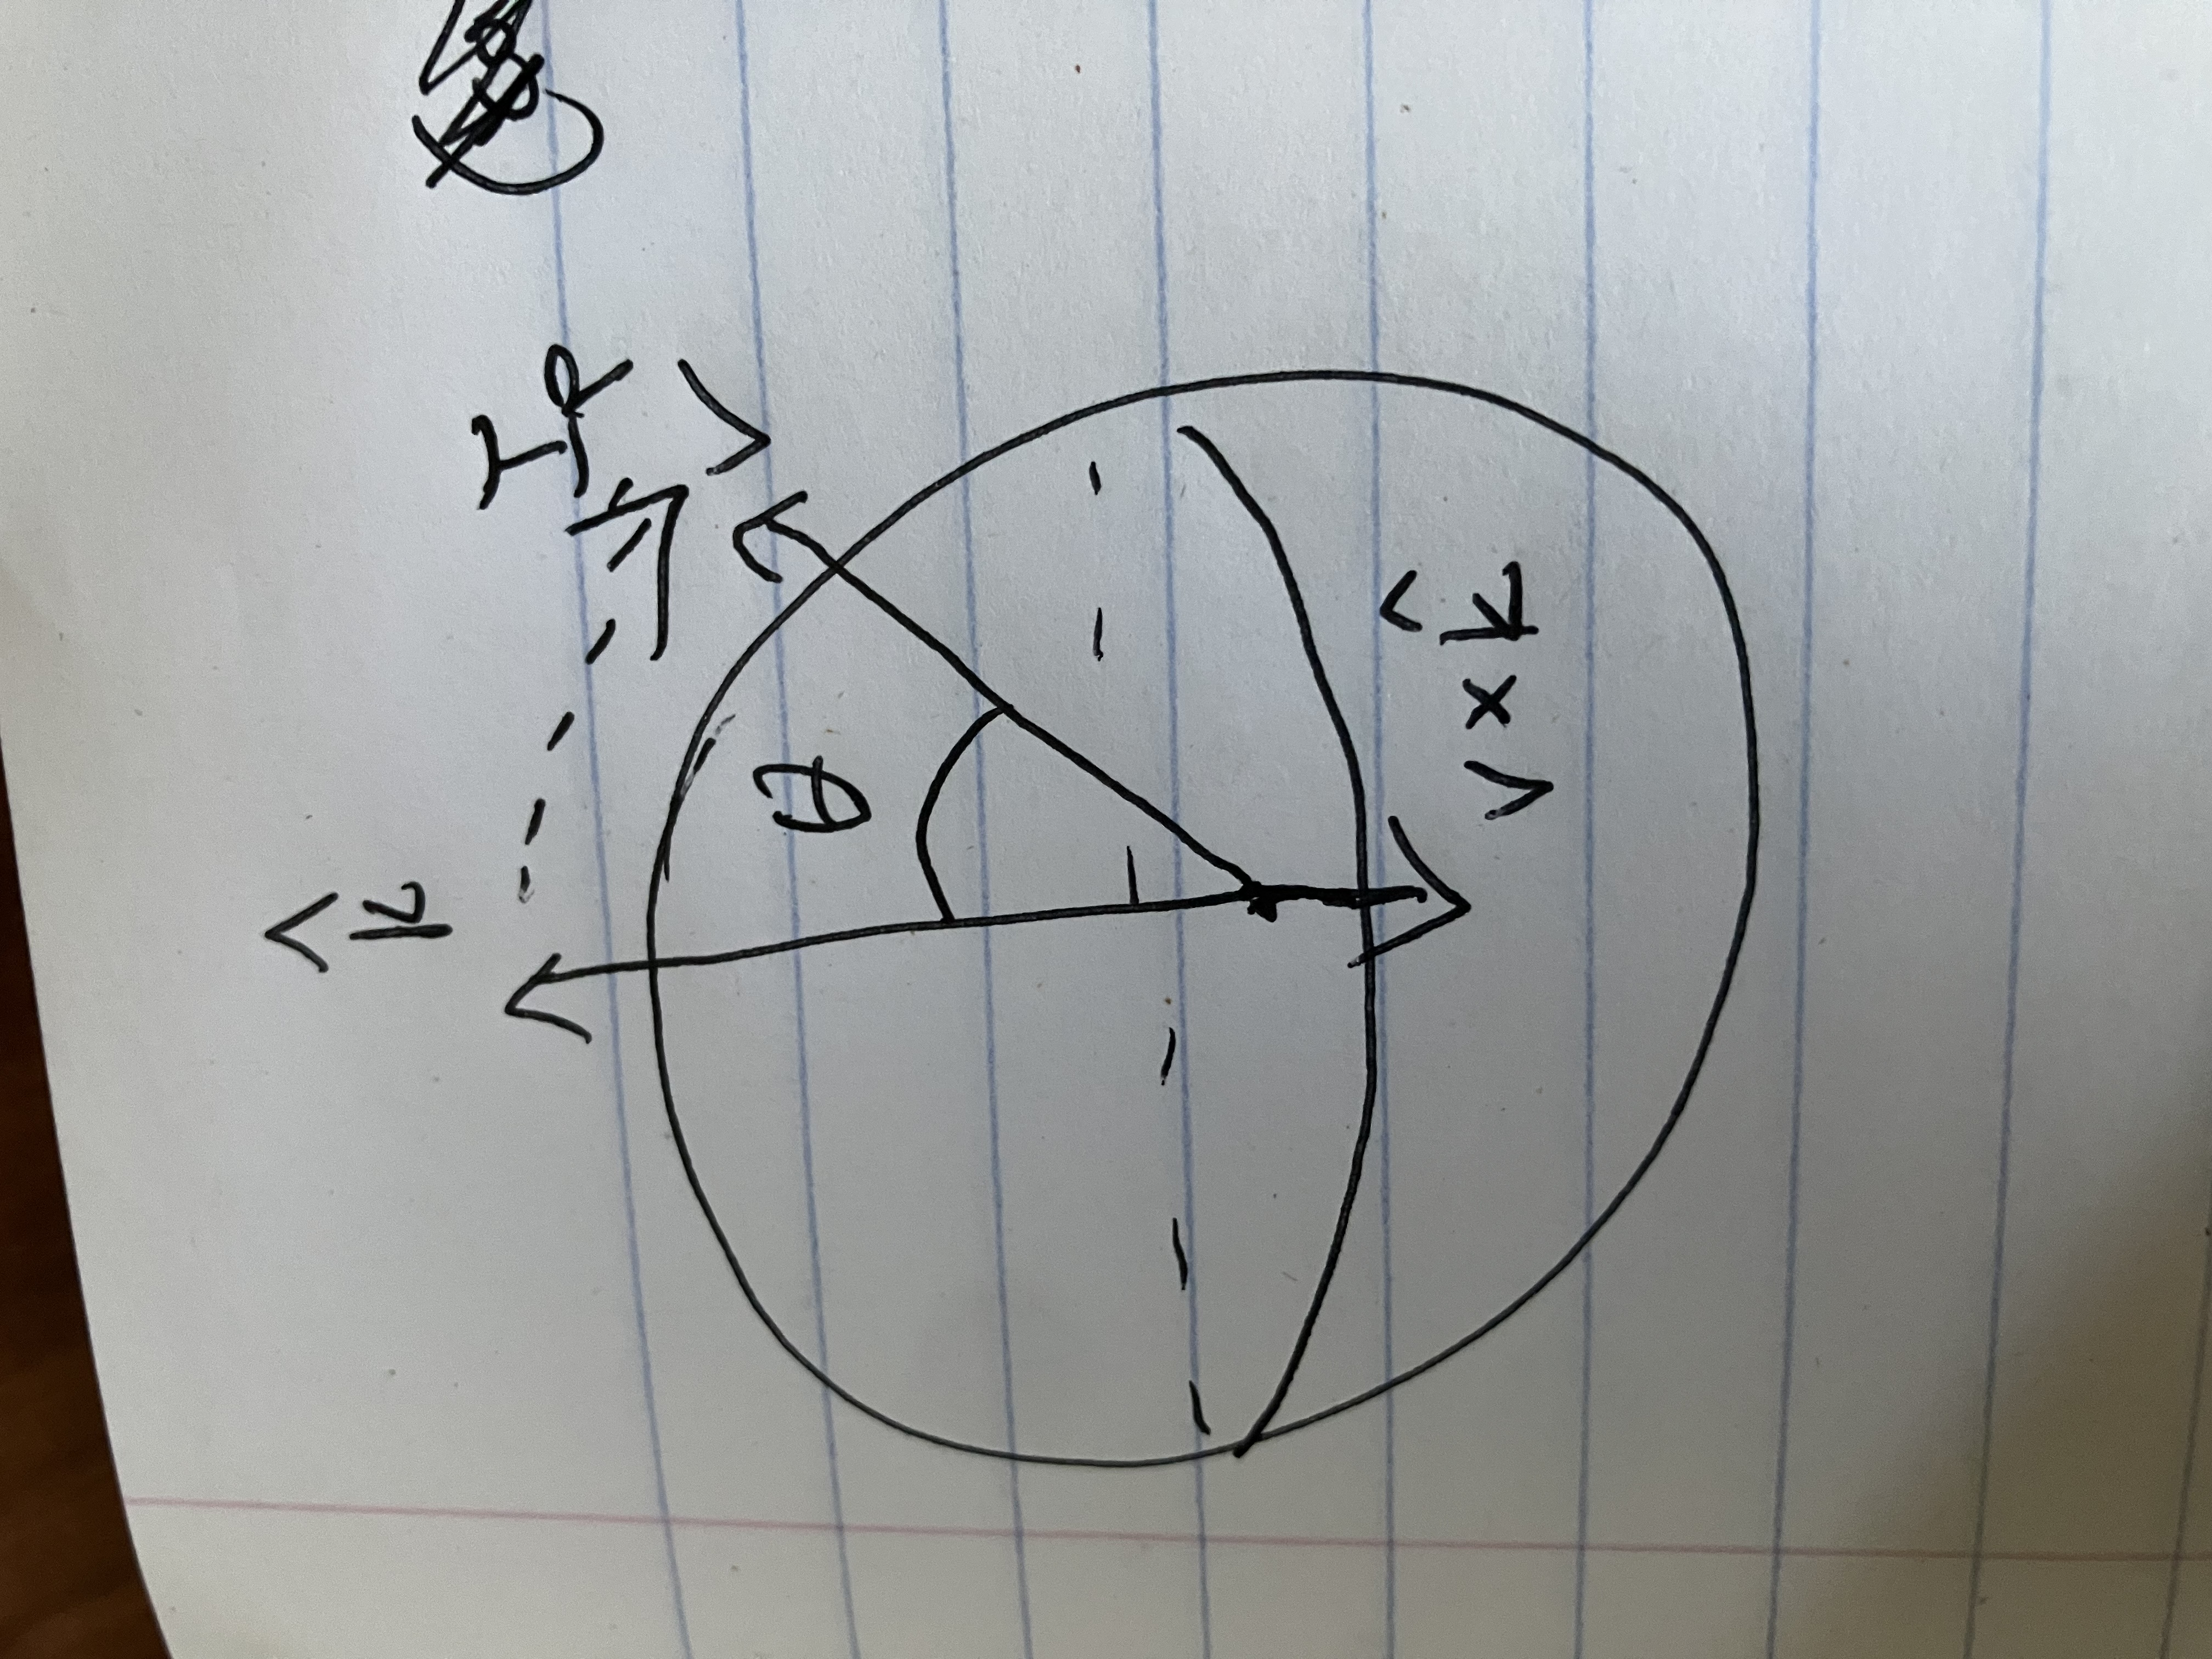
\includegraphics[width=0.8\textwidth,angle=-90,origin=c0]{Images/April 22 - vk ball.png}
    \end{center}

    And we just need to find a rotation so it suffices to find $p \in S^3$ so that 
    \[H(p \khat) = v \implies I_p(H(\khat)) = v \implies I_p(\khat) = v\]
    and then we can just take $p\khat = q$. 

    So to find $p$ we just need to find the rotation axis and the value of $\theta$ in the picture. 

    Generally, $p = \cos \phi + u\sin \phi$ where $\phi = \theta/2$. 

    $u$ is clearly just $\frac{v \times \khat}{\norm{v \times \khat}}$. The only places this fails is $\khat$ and $-\khat$ but we will figure that out later. 

    We know $\theta \in [0, \pi]$ so $\phi \in [0, \pi/2]$. 

    If we say $v = (a, b, c)$ then we can solve for $\cos \phi, \sin \phi, u$: 
    
    First $u$:
    \[u = \frac{ v \times \khat }{\norm{v \times \khat}} = \frac{1}{\norm{v \times \khat}} \begin{vmatrix}
        \ihat & \jhat & \khat\\ 
        a & b & c\\ 
        0 & 0 & 1
    \end{vmatrix} = \frac{1}{\norm{v \times \khat}} (\ihat - a\jhat) = \frac{1}{\sqrt{a^2 + b^2}}(b\ihat - a\jhat)\]

    Now $\cos \phi$: 
    \[v \cdot \khat = \norm v \; \norm \khat \; \cos \theta \implies c = \cos \theta \implies \cos \phi = \cos \frac{\theta}{2} = \sqrt{\frac{1 + \cos \theta}{2}} = \sqrt{\frac{1 + c}{2}}\]

    Finally $\sin \phi$: 
    \[\sin \phi = \sqrt{\frac{1 - \cos \theta}{2}} = \sqrt{\frac{1 - c}{2}}\]

    Therefore, 
    \begin{align*}
        p &= \sqrt{\frac{1 + c}{2}} + \sqrt{\frac{1-c}{2}}\left(\frac{1}{\sqrt{a^2 + b^2}}(b\ihat - a\jhat)\right)\\ 
        &= \frac{1}{\sqrt{2(1 + c)}}\left((1 + c)+ \sqrt{1^2 - c^2}\left(\frac{1}{\sqrt{a^2 + b^2}}(b\ihat - a\jhat)\right) \right)\\ 
        &= \frac{1}{\sqrt{2(1 + c)}}(1 + c + b\ihat - a\jhat)
    \end{align*}

    (Errata: $p = \frac{1}{\sqrt{2(1 + c)}}(1 + c - b\ihat + a\jhat)$ because of orientation of $\{v, \khat, v \times \khat\}$)

\section{April 24:}
    Last class, we drew this diagram: 
    \begin{center}
        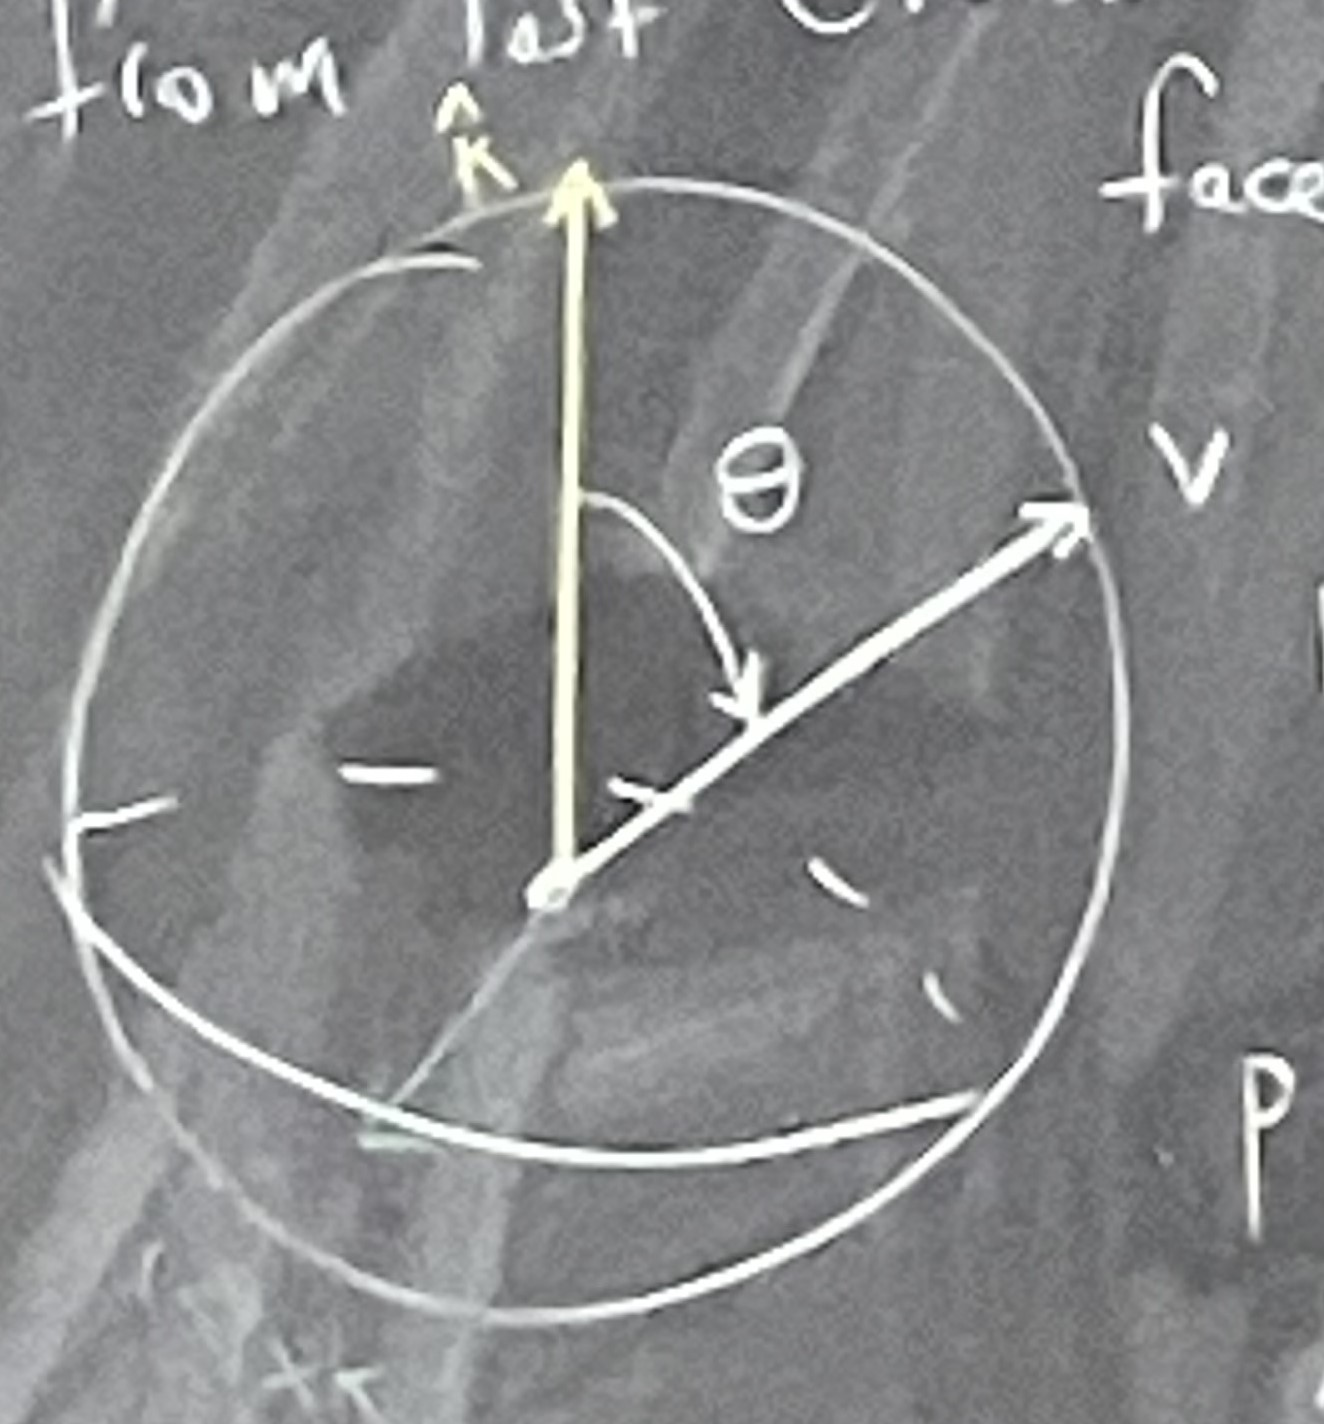
\includegraphics[width=0.8\textwidth,angle=-90,origin=c0]{Images/April 24 - rotation ball.png}
    \end{center}

    Seen face on, the rotation from $\khat$ to $v$ is clockwise. Seen from the back, it is counterclockwise. 

    Since the Euler-Rorigues theorem is stated \emph{clockwise}, $p = \cos \phi + \sin \phi u$ with $\theta = - \theta/2$.

    Last time, we had visuals of some Hopf-fibres. For two generic points in $S^2$, their fibres in $S^3$ will be linked. 
    (explicitly $p, q \in S^2$ will lead to linked circles $H^{-1}\{p\}, H^{-1}\{q\}$ via the maps $H^{-1}: S^2 \to S^3$ and the stereographic projection $S^3 \to \R^3$)

    For all points other than the north pole, 
    \[H^{-1}(\khat) = \cos \theta + \khat \sin \theta\]
    (we have the bad point at $\theta = \pi/2$ and are okay otherwise)

    Since we defined the north pole to be $\khat$, stereographic projection will be a bijection $F: S^3/\khat \biject \R^3$ 

    Where 
    \[F(x, y, z, w) = \left(\frac{x}{1 - w}, \frac{y}{1- w}, \frac{z}{1 - w}\right)\] 

    Which means the fibre at $\khat$ is a line along the $x$-axis and the fibre of $-\khat$ will be a circle in the $yz$-plane. (\emph{{Proof:}} HW. Consider $q\khat q^{-1} = \khat$)

    \begin{center}
        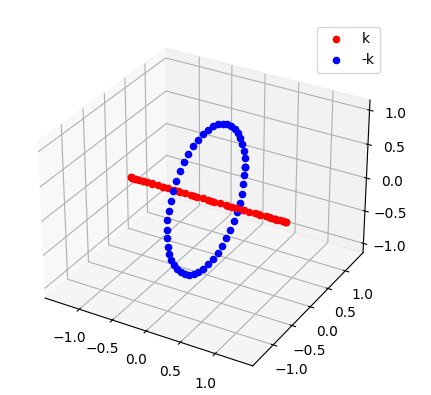
\includegraphics[width=0.8\textwidth]{Images/k fibres.png}
    \end{center}

    Clearly, these are linked. How do we formalize this notion? 

    \textbf{Motivation:} Consider the curve 
    \begin{center}
        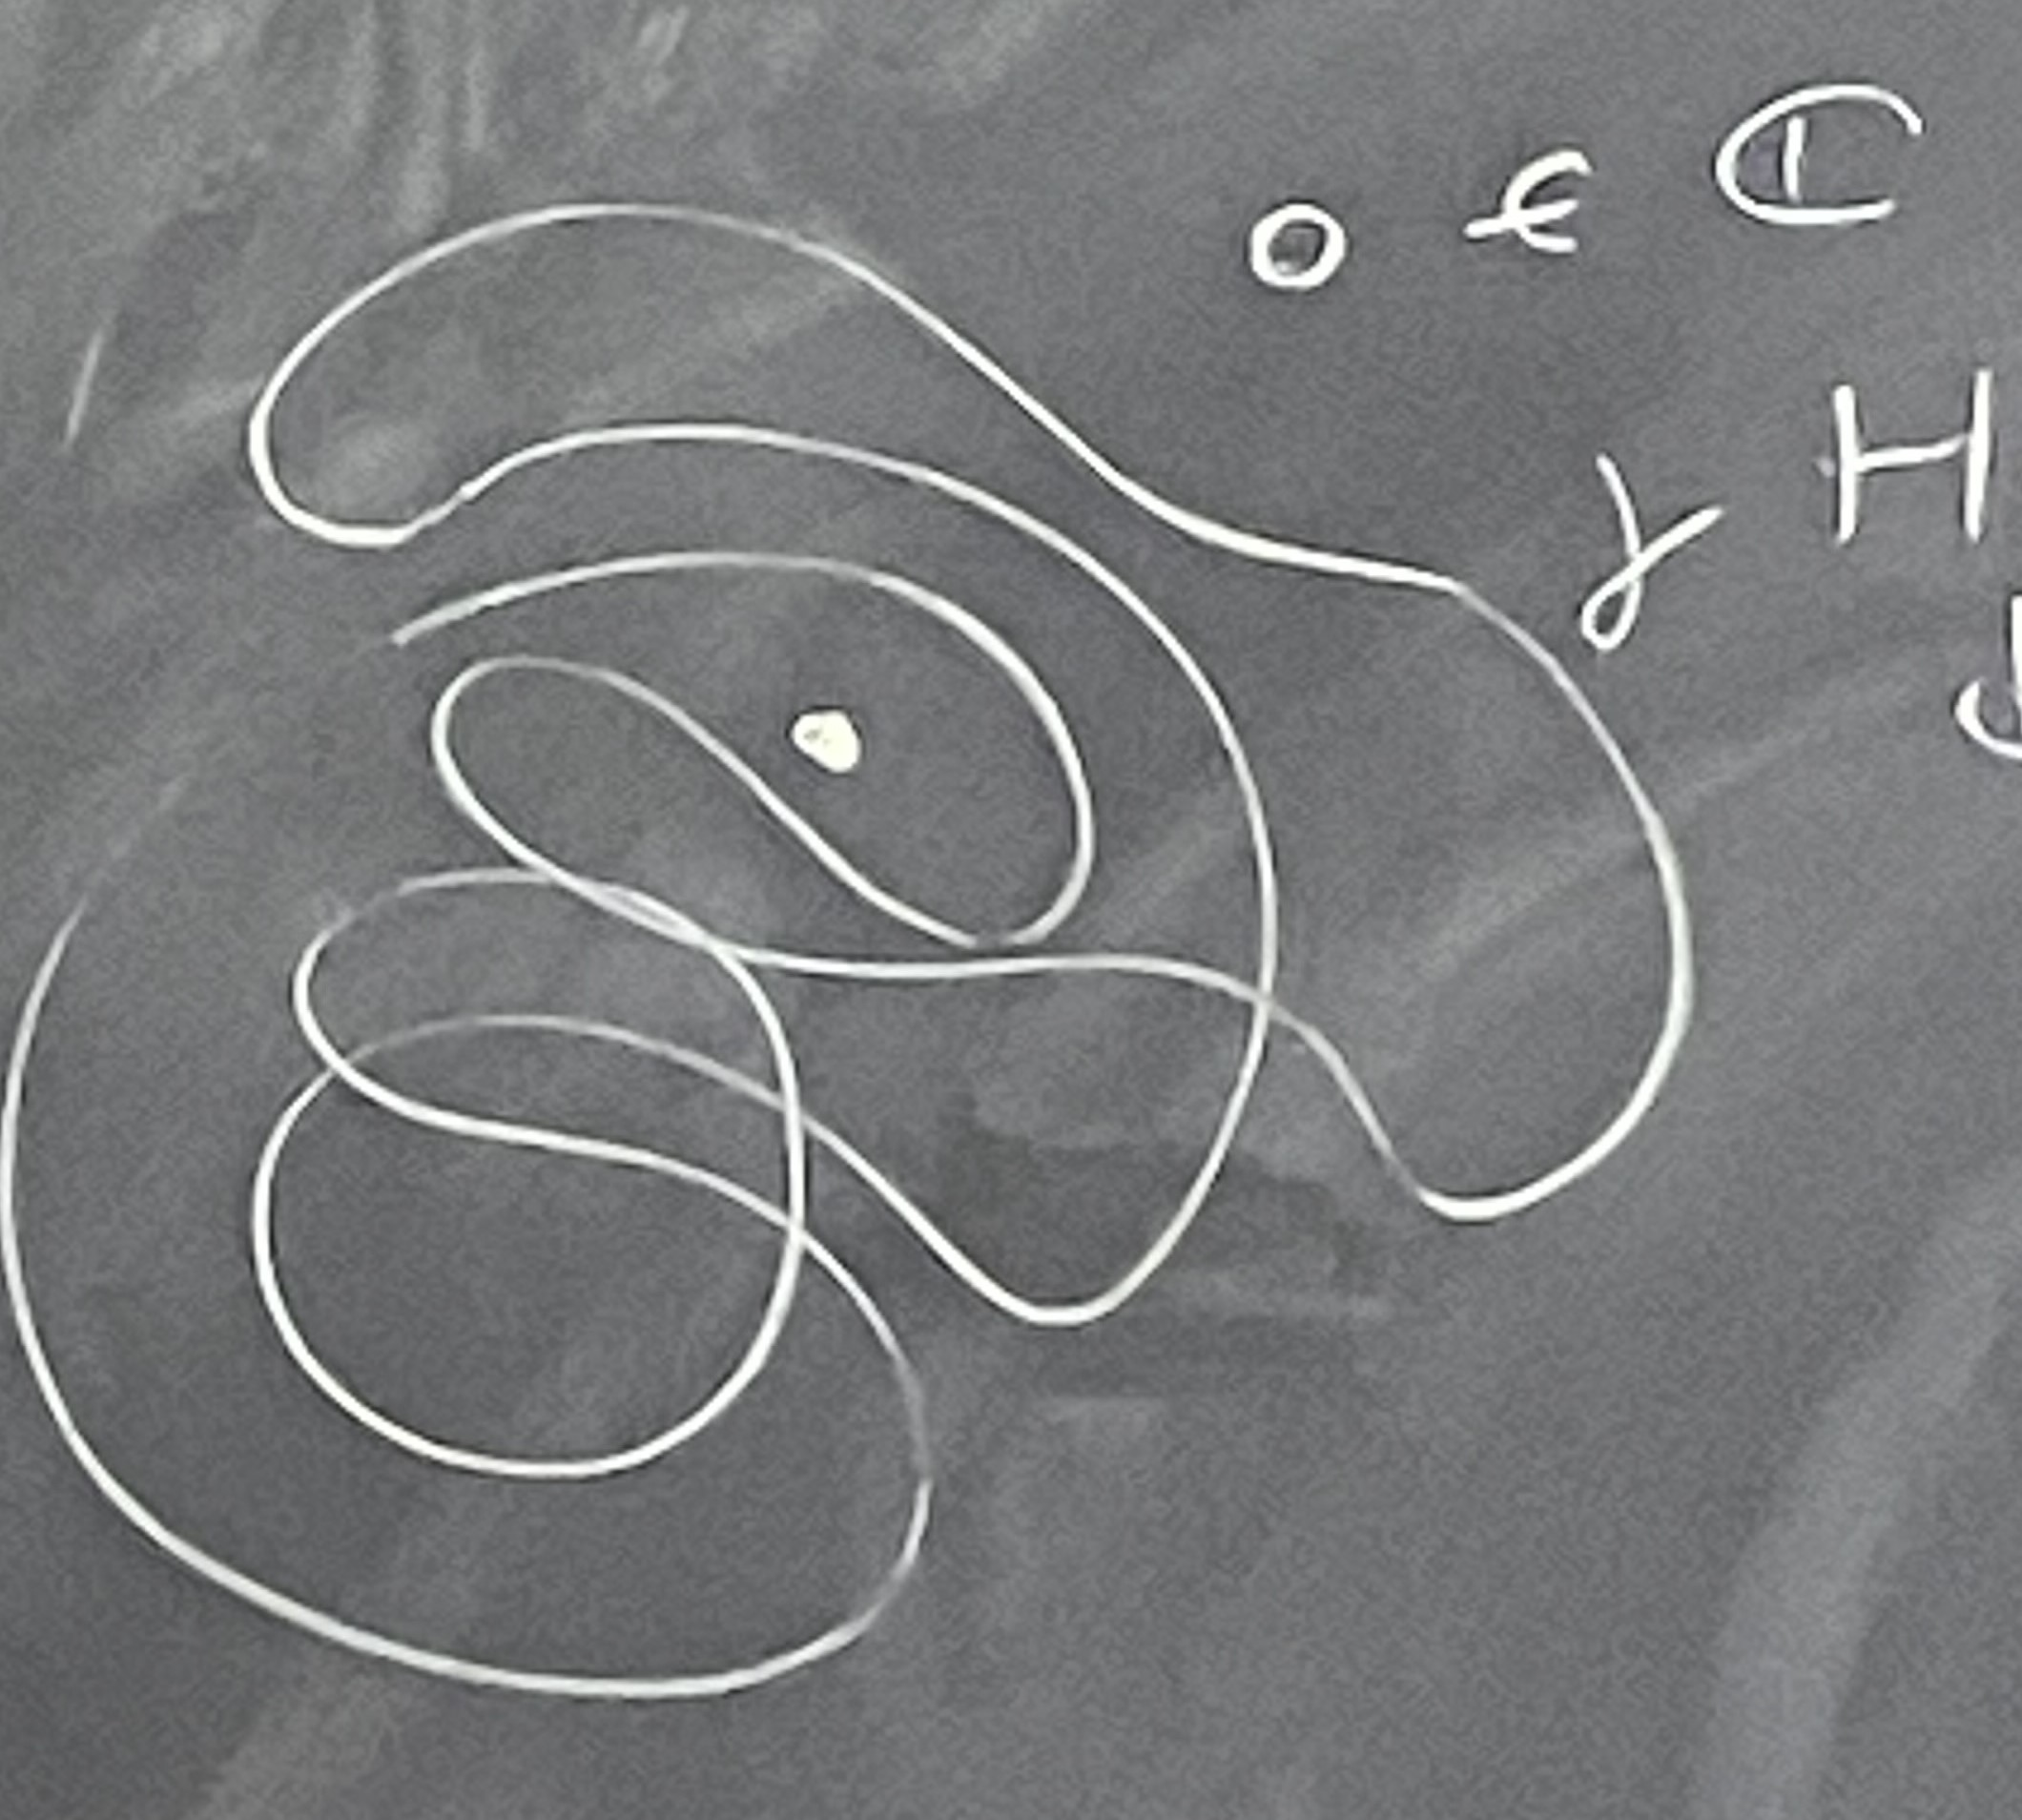
\includegraphics[width=0.8\textwidth]{Images/April 24 - Winding curve}
    \end{center}

    How many times does the curve $\gamma$ wrap around $0$? 

    Explicitly, we want to find the number of oriented wraps around $p$ ($\in \Z$) given a point $p$ and a closed curve $\gamma$ (not through $p$)

    We can consider $\pi_1(s)$, the group of curves at $p \in S$ up to continuous deformation.

    We can imagine picking an orientation on $\R^2/0$ and deforming the curve to wrap around a generator $n$-times where $n$ is our \emph{winding number}. 

    We can also think about this problem geometrically in terms of one-forms. 

    In a sense, we have a function $\R^2/0 \to \R$ which measures the angle relative to $0 \in \R^2$ at a point $p$. If we imagine the vector $\vec{OP}$ as the hypotenuse of a triangle with legs $x, y$, then the angle is $\theta = \arctan(y/x)$. Though unfortunately, this is really only defined locally. But, we can still take a local derivative: 
    \[d\theta = \frac{-y}{x^2 + y^2}\; dx + \frac{x}{x^2 + y^2} \; dy\] 
    which means that we can integrate along curves!
    \[\gamma \mapsto \int_{\gamma} d\theta\]
    but since the curves are closed ($\gamma(0) = \gamma(1)$), 
    \[\int_{\gamma} d\theta = `\theta(\gamma(1)) - \theta(\gamma(0))'\]

    \textbf{Example:} 
    \begin{align*}
        \gamma(t) &= ( \cos t, \sin t), \quad t \in [0, 2\pi]\\ 
        \int_\gamma d\theta &= \frac{1}{2\pi}\int_0^{2\pi} \frac{-\sin t}{\sin^2 t + \cos^2 t} \; d(\cos t) + \frac{\cos t}{\sin^2 t + \cos^2 t} \; d(\sin t)\\
        &= \frac{1}{2\pi}\int_0^{2\pi} \sin t(\sin t) + \cos t \cos t \; dt\\ 
        &= \frac{1}{2\pi}\int_0^{2\pi} 1 \; dt = 1
    \end{align*}

    So 
    \[\omega = \frac{1}{2\pi}\begin{pmatrix}
        -y & dx\\ 
        x & dy
    \end{pmatrix} \frac{1}{x^2 + y^2}\]
    where $[\omega]$ generates $H'(\R^2/p)$

    \textbf{Question:} Why is there no honest function $f: \R^2/O \to \R$ so that $df = \omega$? 

    Because then $\int_{\gamma} d\theta = \theta(\gamma(1)) - \theta(\gamma(0)) = 0$ exactly. But our calculation just showed that $\int_{\gamma}d\theta \neq 0$ 

    We want to understand why linked and unlinked curves are fundamentally different in order to understand why $H^{-1}(p)$ and $H^{-1}(q)$ (for distinct $p, q$) are linked. 

    First reduction: consider $p, q \in S^2$ and their fibres. We claim it suffices to show instead that $p = \khat, q = -\khat$. 

    Intuitively, the linkage of fibres in invariant under isotopy (under deformation, what is linked should stay linked and vice versa.) Therefore, if we move $p$ to $\khat$ and $q$ to $-\khat$, the linkage should remain.

    If we imagine two curves around two parallel lines: 
    \begin{center}
        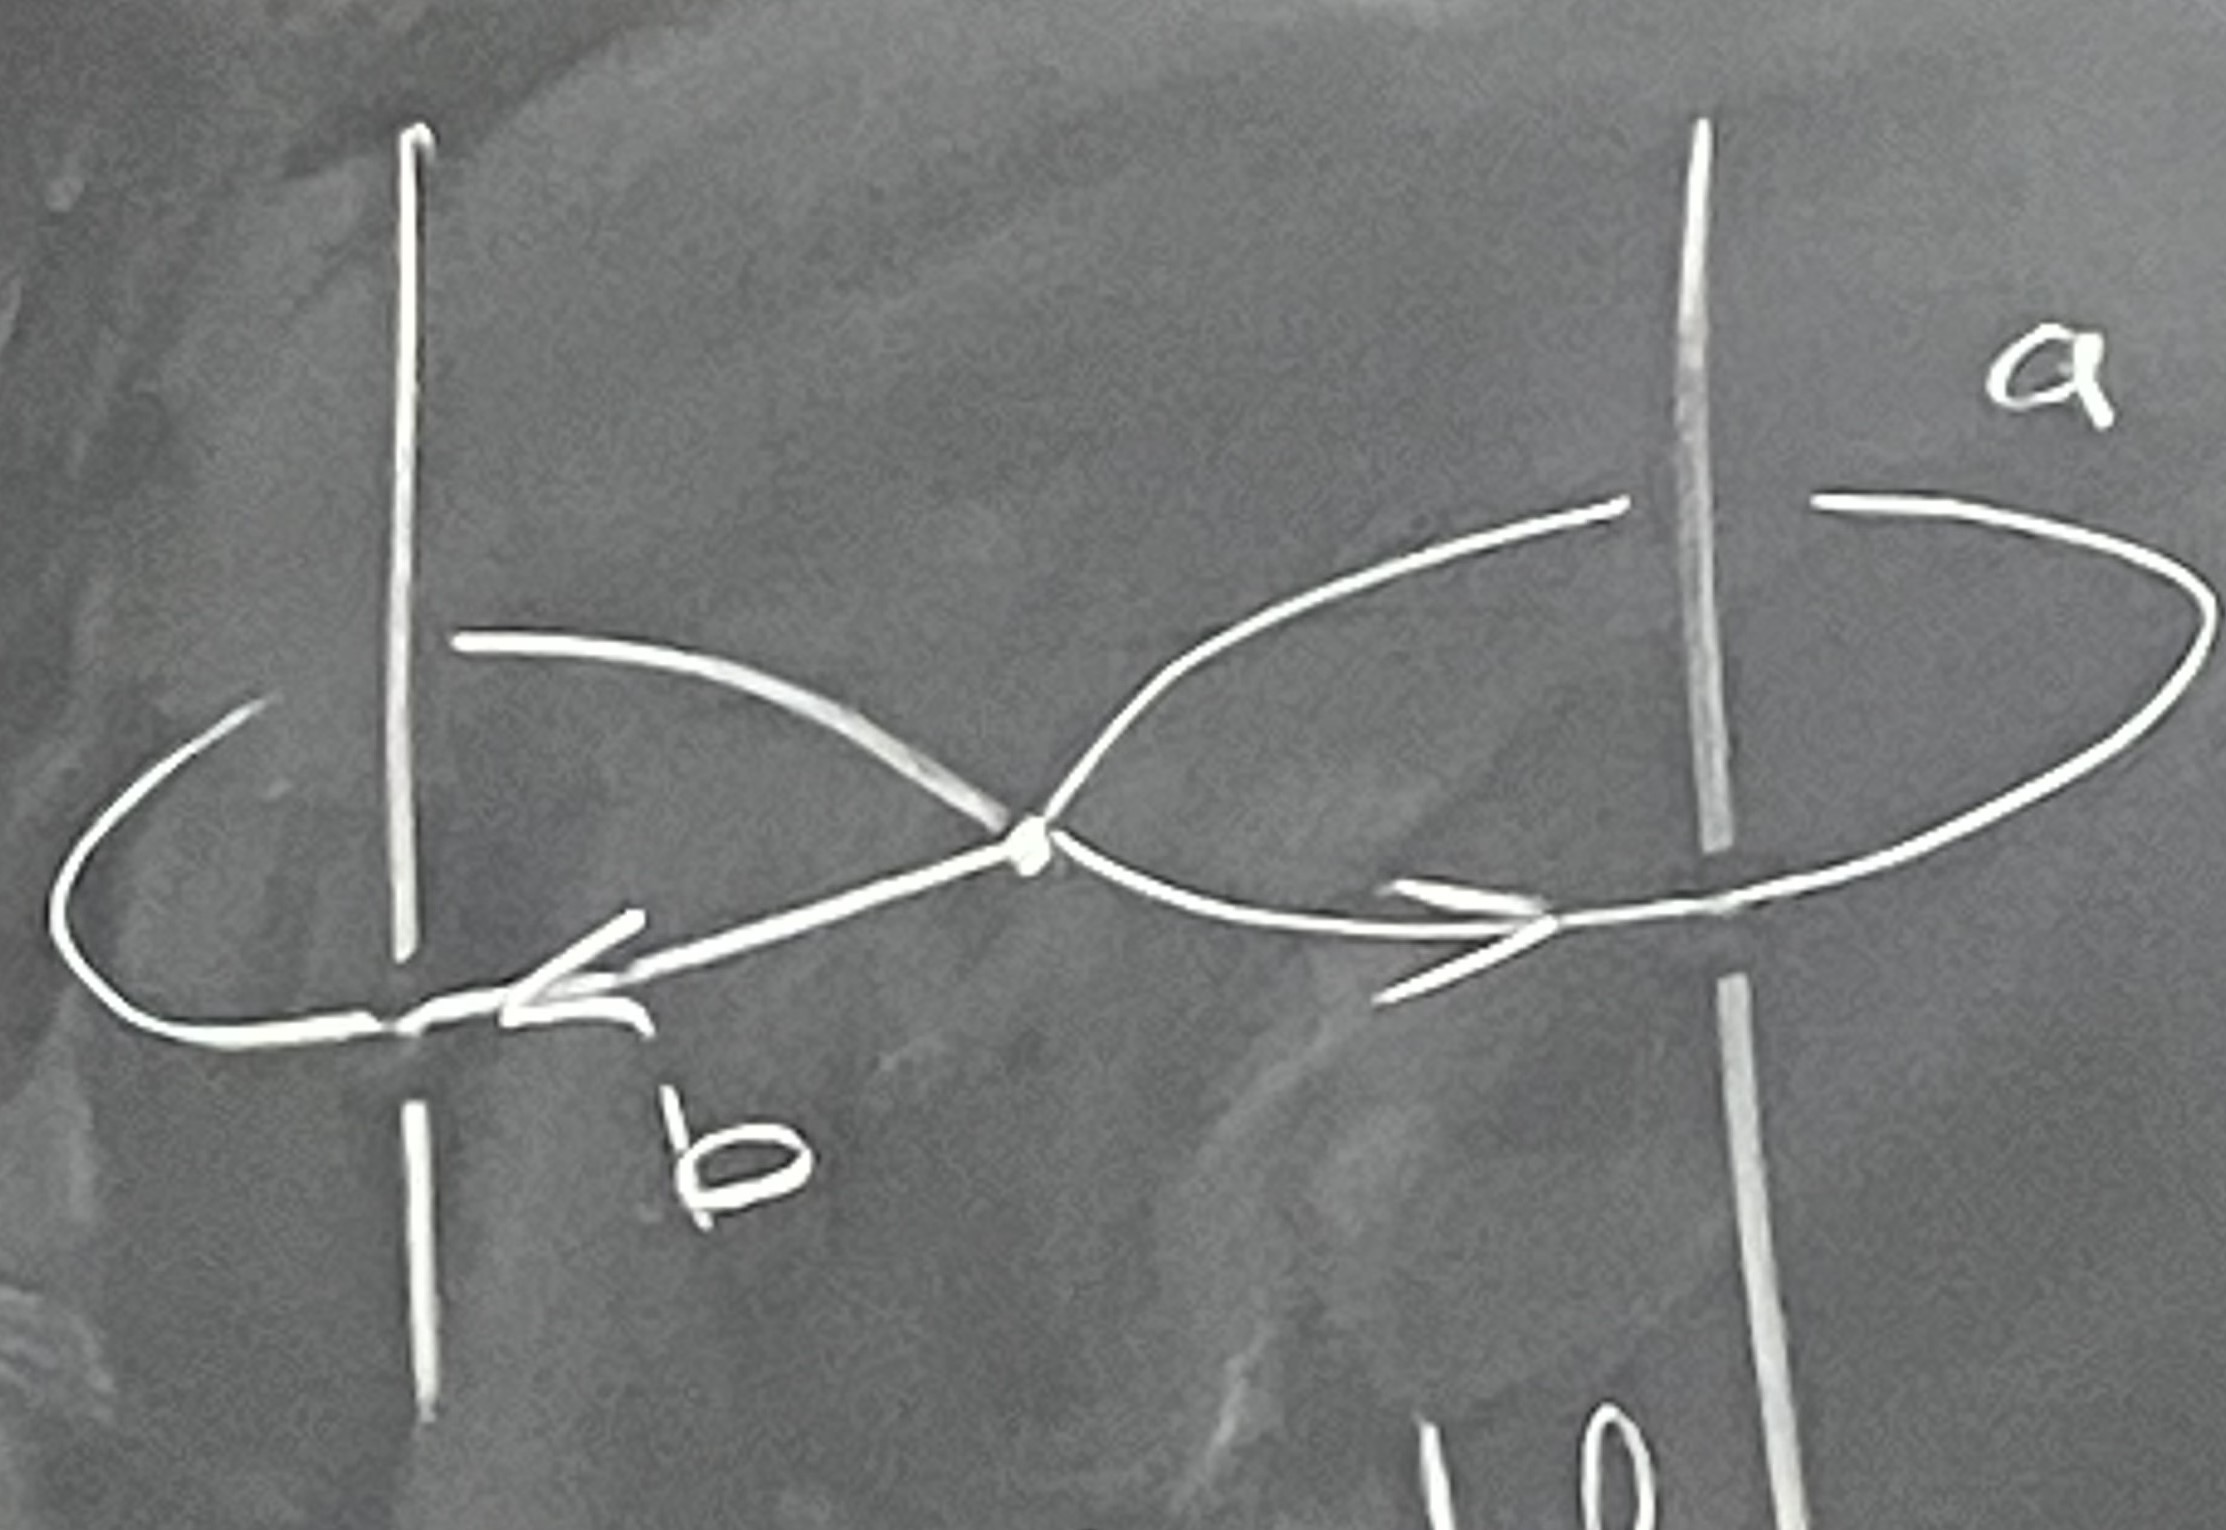
\includegraphics[width=0.8\textwidth]{Images/April 24 - Parallel lines.png}
    \end{center}

    Then, clearly, there is no way to defom $a$ to $b$. In fact, $a, b$ generate a free group in $\pi_1(\R^3/\text{two parallel lines})$ 

    \textbf{Application:} How do you hang a picture with two nails such that pulling either nail causes the picture to drop? 

    This problem resolves to finding a non-trivial relation on the generating circles $a, b$ of two linked circles.

    If we imagine the curve formed by the word $aba^{-1}b^{-1}$ from the generating point, we have 
    \begin{center}
        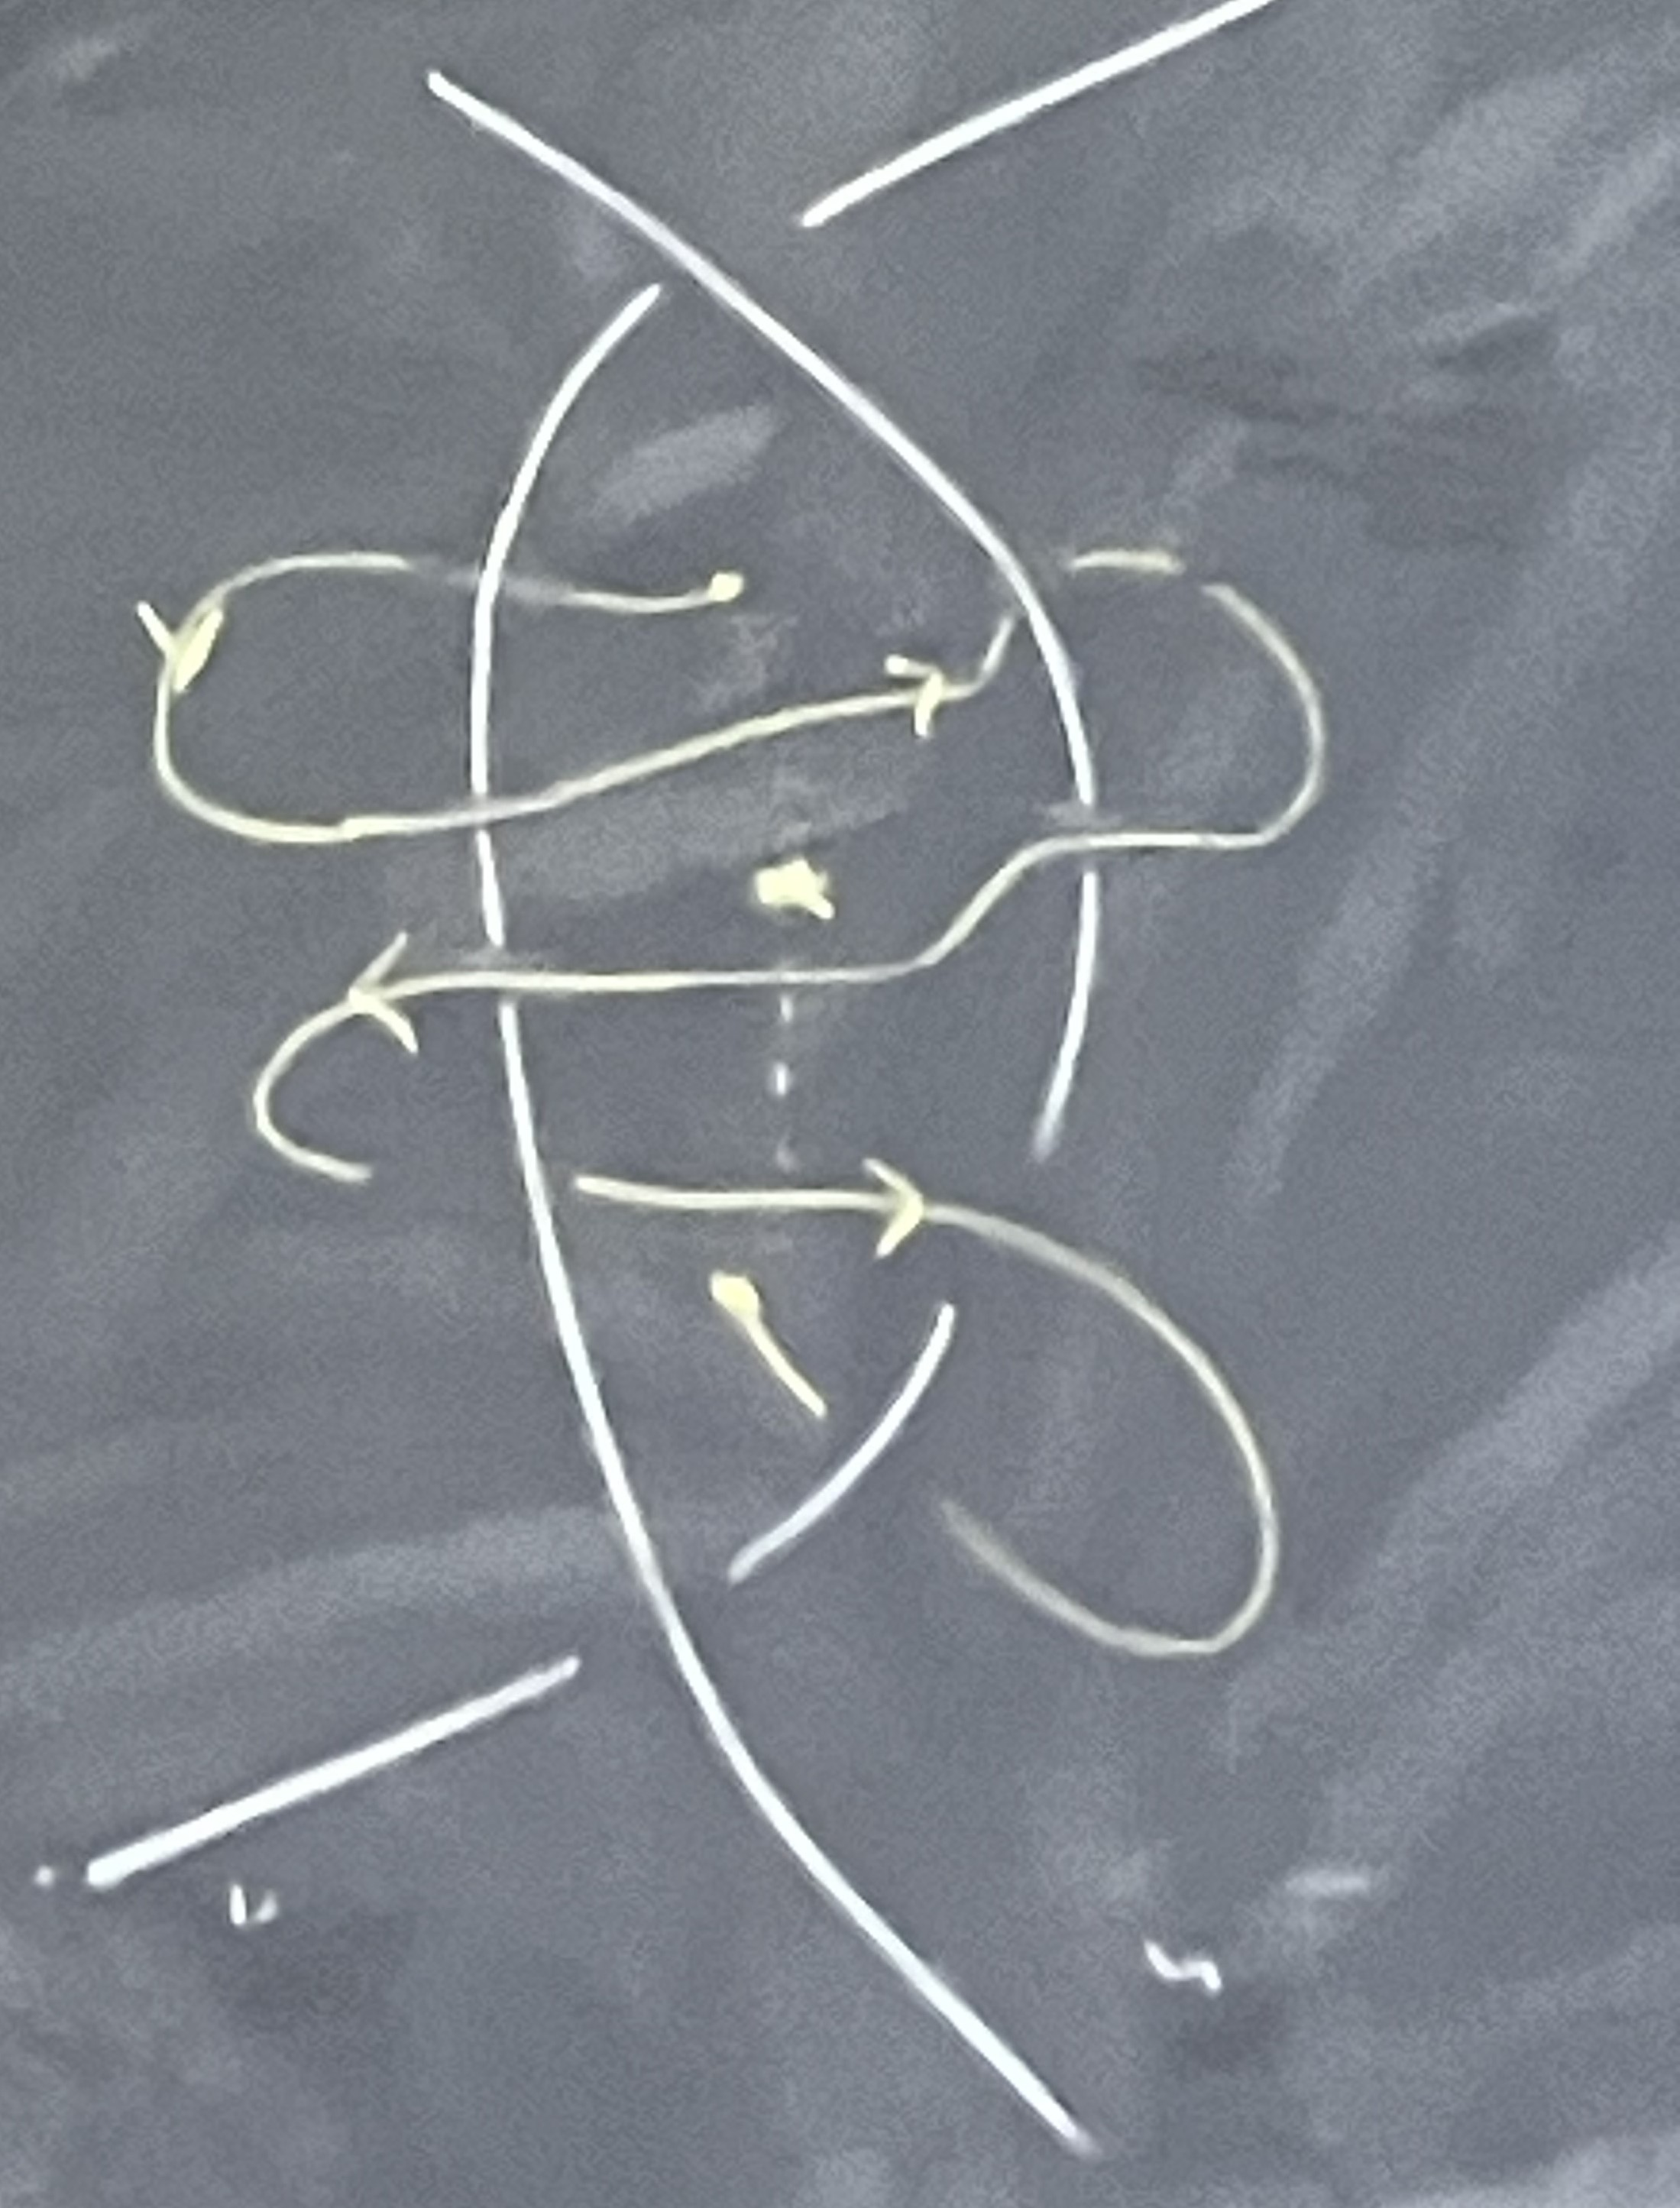
\includegraphics[width=0.8\textwidth]{Images/April 24 - Word 1.png}
    \end{center}

    But now we can shift the entire thing to the other side of the left circle giving us this image:
    \begin{center}
        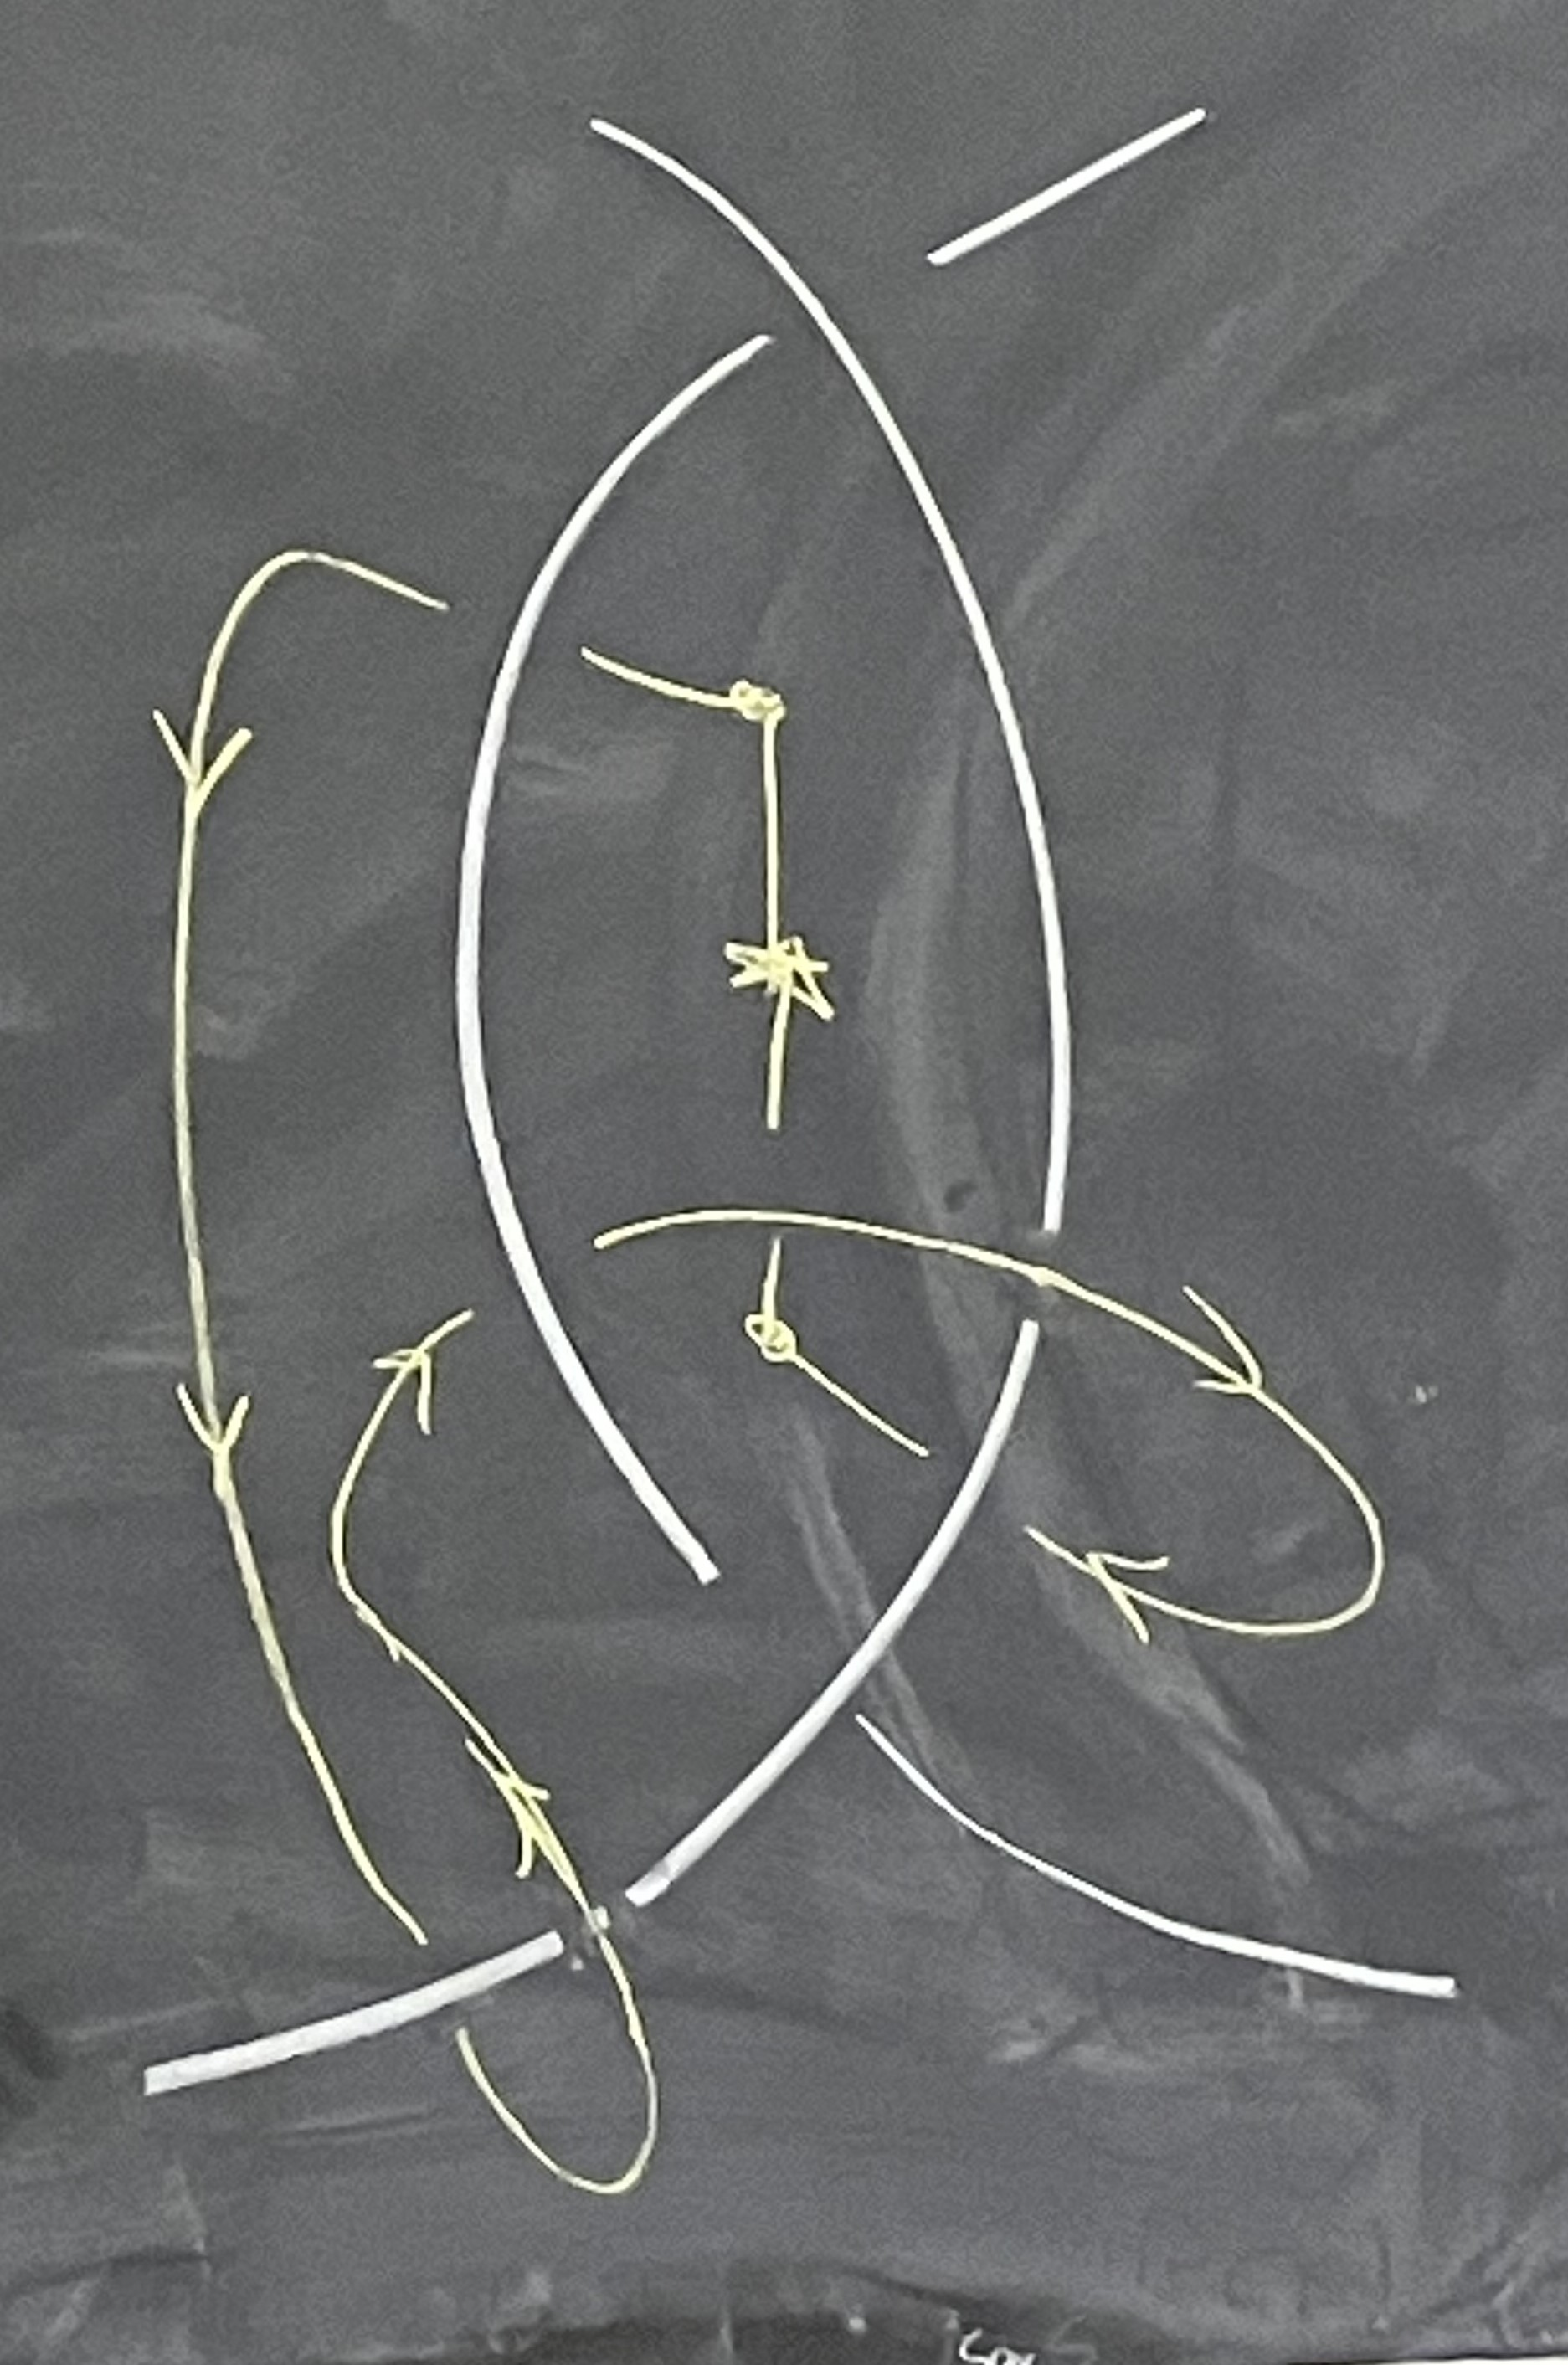
\includegraphics[width=0.8\textwidth]{Images/April 24 - Word 2.png}
    \end{center}

    Now we can free the yellow curve by taking the loop on the right and again twisting it to the left side, then taking the last part down. 
    
    This shows that $1 = aba^{-1}b^{-1}$ so 
    \[\pi_1(\R^3/\text{linked circles}) \simeq \Z^2\]

\end{document}

